%% ============================================================
%% Distribution-Free Prediction Intervals for Seasonally
%% Heteroskedastic Time Series
%%
%% Lucas Rafael de Andrade
%% [Affiliation TBD]
%%
%% Target: Brazilian Review of Econometrics / Estudos Econômicos
%% ============================================================

\documentclass[12pt,a4paper]{article}

% --- Encoding & language ---
\usepackage[T1]{fontenc}
\usepackage[utf8]{inputenc}
\usepackage[english]{babel}

% --- Math ---
\usepackage{amsmath}
\usepackage{amsthm}
\usepackage{amssymb}
\usepackage{mathtools}   % dcases, coloneqq, etc.
\usepackage{bm}          % \bm for bold math

% --- Layout ---
\usepackage[margin=2.5cm]{geometry}
\usepackage{microtype}
\usepackage{setspace}
\onehalfspacing

% --- Figures & tables ---
\usepackage{graphicx}
\usepackage{booktabs}
\usepackage{array}
\usepackage{multirow}
\usepackage[font=small,labelfont=bf]{caption}
\usepackage{subcaption}
\usepackage{float}

% --- Algorithms ---
\usepackage[ruled,vlined,linesnumbered]{algorithm2e}

% --- Bibliography ---
\usepackage[round,authoryear]{natbib}
\bibliographystyle{apalike}

% --- Hyperlinks (load last among these) ---
\usepackage[colorlinks=true,
            linkcolor=blue!60!black,
            citecolor=blue!60!black,
            urlcolor=blue!60!black]{hyperref}

% --- Lists ---
\usepackage{enumitem}

% --- Check/cross marks (for simulation summary table) ---
\usepackage{pifont}
\newcommand{\cmark}{\ding{51}}
\newcommand{\xmark}{\ding{55}}

% --- Internal comments (remove before submission) ---
\usepackage{xcolor}
\newcommand{\todo}[1]{\textcolor{red}{\textbf{[TODO: #1]}}}
\newcommand{\note}[1]{\textcolor{blue!70!black}{\textbf{[NOTE: #1]}}}

% ============================================================
%  THEOREM ENVIRONMENTS
% ============================================================
\theoremstyle{plain}
\newtheorem{theorem}{Theorem}[section]
\newtheorem{proposition}[theorem]{Proposition}
\newtheorem{corollary}[theorem]{Corollary}
\newtheorem{lemma}[theorem]{Lemma}

\theoremstyle{definition}
\newtheorem{definition}[theorem]{Definition}
\newtheorem{assumption}{Assumption}
\newtheorem{algorithm_def}[theorem]{Algorithm}  % named differently to avoid clash

\theoremstyle{remark}
\newtheorem{remark}[theorem]{Remark}
\newtheorem{example}[theorem]{Example}

% ============================================================
%  NOTATION MACROS
%  (all notation is defined here; never hard-code in text)
% ============================================================

% --- Sets and indices ---
\newcommand{\calT}{\mathcal{T}}       % index set T_s for stratum s
\newcommand{\calA}{\mathcal{A}}       % prediction algorithm
\newcommand{\calF}{\mathcal{F}}       % filtration
\newcommand{\N}{\mathbb{N}}
\newcommand{\R}{\mathbb{R}}

% --- Time series quantities ---
\newcommand{\Yt}{Y_t}                  % response at t
\newcommand{\Xt}{X_t}                  % feature vector at t
\newcommand{\eps}{\epsilon_t}          % true error at t
\newcommand{\epshat}{\hat{\epsilon}}   % estimated (LOO) residual
\newcommand{\fhat}{\hat{f}}            % trained predictor
\newcommand{\floo}{\hat{f}_{-t}}       % LOO predictor at t

% --- CDFs ---
\newcommand{\Ft}{F_t}                  % true CDF of epsilon_t
\newcommand{\Fs}{F_s}                  % CDF of season s
\newcommand{\Fbar}{\bar{F}}            % pooled (average) CDF
\newcommand{\Ftilde}{\tilde{F}}        % empirical CDF of true errors
\newcommand{\Fhat}{\hat{F}}            % empirical CDF of LOO residuals
\newcommand{\FhatS}{\hat{F}_{s^*}}     % stratified empirical CDF

% --- Prediction intervals ---
\newcommand{\Chat}{\hat{C}_{t}^{\alpha}}              % EnbPI interval at t
\newcommand{\Chatpool}{\hat{C}_{t}^{\alpha,\text{pool}}}   % pooled
\newcommand{\Chatstrat}{\hat{C}_{t}^{\alpha,\text{strat}}} % stratified
\newcommand{\Coracle}{C_{t}^{\alpha}}                 % oracle interval

% --- Seasonal quantities ---
\newcommand{\sstar}{s^*}               % season of prediction point T+1
\newcommand{\Sper}{S}                  % seasonal period
\newcommand{\Ts}{T_{\sstar}}           % stratum size for season s*
\newcommand{\bsstar}{b_{\sstar}}       % seasonal bias
\newcommand{\sigt}{\sigma_{s(t)}}      % seasonal standard deviation
\newcommand{\sigs}{\sigma_s}           % std at season s

% --- Estimation quality ---
\newcommand{\deltaT}{\delta_T}         % estimation quality (full sample)
\newcommand{\deltaTs}{\delta_{\Ts}}    % estimation quality (stratum)

% --- Quantiles & p-values ---
\newcommand{\betahat}{\hat{\beta}}     % optimal lower quantile
\newcommand{\phat}{\hat{p}_{T+1}}     % empirical p-value
\newcommand{\Quant}[2]{Q_{#1}\!\left(#2\right)} % Q_alpha(set)

% --- Other ---
\newcommand{\abs}[1]{\left|#1\right|}
\newcommand{\norm}[1]{\left\|#1\right\|}
\newcommand{\Ind}[1]{\mathbf{1}\!\left\{#1\right\}}
\newcommand{\E}{\mathbb{E}}
\newcommand{\Prob}{\mathbb{P}}
\newcommand{\given}{\,\middle|\,}

% ============================================================
%  DOCUMENT
% ============================================================
\begin{document}

% --- Title ---
\title{Distribution-Free Prediction Intervals for Seasonally
       Heteroskedastic Time Series\thanks{%
         Acknowledgements TBD.
         Replication code available at
         \url{https://github.com/Andrade020/enbpi-seasonal}.}}

\author{Lucas Rafael de Andrade\thanks{%
        [Affiliation TBD]. E-mail: \texttt{[TBD]}.}}

\date{\today}

\maketitle

% ============================================================
\begin{abstract}
% ============================================================
% ABSTRACT
% ============================================================
Pooled calibration of conformal prediction intervals, as in the
Ensemble Batch Prediction Intervals (EnbPI) algorithm of
\citet{xu2023conformal}, carries a persistent bias under seasonal
heteroskedasticity: the per-season coverage gap contains a term
$2b_{s^*}$, which measures the discrepancy between the season-specific
and the pooled residual distribution and does not vanish as the sample
grows, so that volatile seasons are systematically undercovered.  Two
schemes remove it, and they are the endpoints of a one-parameter
family: stratifying the calibration buffer by season, and standardising
residuals by a season-specific scale before pooling them.  The second
is the more efficient of the two, and it is valid only when the seasons
differ in scale alone; when they differ in the shape of the error
distribution it leaves the coverage spread where pooling left it, while
stratification cuts it by two thirds.

Stratification is usually thought too expensive at the per-season
sample sizes a monthly series provides, and we show that most of that
expense belongs to the interval construction rather than to the
conditioning.  The empirical quantile of a short buffer is biased
inwards, and the minimum-width line search selects the narrowest of
many candidate quantile pairs computed from the same residuals, which
alone costs four to six percentage points of coverage at these buffer
lengths.  Building the interval from conformal order statistics with a
fixed asymmetry repairs both, and stratified coverage at twenty
residuals per season then rises from $0.79$ to its nominal $0.90$ in
four different seasonal designs, the residual cost being width rather
than coverage.  On the food-at-home component of the Brazilian consumer
price index (IPCA; BCB series 1635, $T_s = 20$) the same change takes
coverage from $79.2\%$ to exactly $90.0\%$ with no dispersion across
the twelve calendar months, and on monthly export growth (BCB series
1402, $T_s = 35$) it raises the worst month from $70\%$ to $90\%$ and
overall coverage from $86.7\%$ to $95.0\%$, the overshoot being the
conservatism of an interval whose endpoints are still the extremes of
its buffer.  A permutation test rejects the pure-scale restriction on
both series.

\bigskip

\noindent\textbf{Resumo:}
\begin{otherlanguage}{brazilian}%
A calibração conjunta (\emph{pooled}) de intervalos conformes, como no
algoritmo EnbPI de \citet{xu2023conformal}, carrega um viés persistente
sob heteroscedasticidade sazonal: a lacuna de cobertura por estação
contém um termo $2b_{s^*}$ que não desaparece à medida que a amostra
cresce, de forma que as estações voláteis ficam sistematicamente
subcobertas.  Dois esquemas o eliminam, e são os extremos de uma
família de um parâmetro: estratificar o buffer de calibração por
estação, ou padronizar os resíduos por uma escala específica de cada
estação antes de agrupá-los.  O segundo é o mais eficiente dos dois,
porém só é válido quando as estações diferem apenas em escala; quando
diferem na forma da distribuição dos erros, ele deixa a dispersão da
cobertura onde a calibração conjunta a deixou, ao passo que a
estratificação a reduz em dois terços.

Costuma-se considerar a estratificação cara demais para os tamanhos
amostrais por estação de uma série mensal, e mostramos que a maior
parte desse custo pertence à construção do intervalo, e não ao
condicionamento.  O quantil empírico de um buffer curto é enviesado
para dentro, e a busca por largura mínima seleciona o par de quantis
mais estreito entre muitos candidatos calculados dos mesmos resíduos, o
que sozinho custa de quatro a seis pontos percentuais de cobertura
nesses tamanhos.  Construir o intervalo a partir de estatísticas de
ordem conformes, com assimetria fixa, corrige as duas coisas, e a
cobertura estratificada com vinte resíduos por estação sobe então de
$0{,}79$ para o nominal $0{,}90$ em quatro desenhos sazonais
diferentes, sendo o custo remanescente de largura, e não de cobertura.
No componente de Alimentação no domicílio do IPCA (BCB série 1635,
$T_s = 20$), a mesma mudança leva a cobertura de $79{,}2\%$ para
exatamente $90{,}0\%$, sem dispersão entre os doze meses do calendário;
no crescimento mensal das exportações (BCB série 1402, $T_s = 35$), ela
eleva o pior mês de $70\%$ para $90\%$.  Um teste de permutação rejeita
a restrição de escala pura nas duas séries.
\end{otherlanguage}

\end{abstract}

\noindent\textbf{Keywords:} conformal prediction; prediction intervals;
seasonal heteroskedasticity; distribution-free inference; IPCA.

\noindent\textbf{JEL Classification:} C14; C22; C53.

\newpage
\tableofcontents
\newpage

% ============================================================
% ============================================================
% SECTION 1 — INTRODUCTION
% ============================================================
\section{Introduction}
\label{sec:introduction}

Reliable prediction intervals are indispensable whenever
point forecasts are deployed in high-stakes settings: monetary
policy decisions hinge on the uncertainty around inflation
projections; energy-market participants require interval estimates
that correctly reflect demand volatility in winter versus summer;
supply-chain planners need intervals that are not systematically
too narrow in peak months.  In all these settings the key
feature is \emph{seasonal heteroskedasticity}: the variability
of forecast errors differs systematically by calendar month
or quarter.

The conformal-prediction literature has made substantial progress
in constructing prediction intervals for time series
\citep{xu2023conformal, xu2023sequential, barber2023conformal},
but the problem of \emph{seasonal} heteroskedasticity has
received comparatively little attention.  The standard
approach, which we call \emph{pooled calibration},
calibrates intervals on a single buffer of residuals drawn
from all seasons indiscriminately.  When the distribution of
forecast errors varies by season, pooled calibration introduces
a persistent, season-dependent bias: intervals are too narrow
(undercoverage) in volatile seasons and too wide (overcoverage)
in stable seasons, regardless of how large the training set is.

\paragraph{Contribution.}
This paper makes three contributions.

\begin{enumerate}[label=(\roman*)]
\item \emph{Formalisation of the seasonal bias.}
  We derive an explicit upper bound for the per-season
  coverage gap of the pooled EnbPI algorithm
  \citep{xu2023conformal}.  The bound separates into a
  vanishing sampling term and a non-vanishing bias term
  $2b_{s^*}$, where $b_{s^*} = \sup_x |F_{s^*}(x) - \bar{F}(x)|$
  measures the CDF discrepancy between season $s^*$ and the
  pooled residual distribution
  (Proposition~\ref{prop:pooled_gap}).

\item \emph{The \texttt{EnbPI-S} algorithm.}
  We introduce \texttt{EnbPI-S} (Algorithm~\ref{alg:enbpis}),
  a stratified extension of EnbPI that maintains $\Sper$ separate
  calibration buffers (one per calendar season).  The only
  departure from EnbPI is in the calibration step: the line
  search for the optimal asymmetric quantile pair uses only
  residuals from the same season as the prediction target.
  The training phase is unchanged; no data splitting is required;
  and the total memory footprint is identical to EnbPI.

\item \emph{Theoretical guarantees.}
  We prove that the per-season coverage gap of \texttt{EnbPI-S}
  converges to zero at rate $O(\sqrt{\log T_s / T_s})$, where
  $T_s = T/\Sper$ is the per-stratum training size
  (Theorem~\ref{thm:strat_coverage}).
  We also derive the dominance condition
  (Proposition~\ref{prop:strat_dominance})
  under which \texttt{EnbPI-S} has a strictly tighter bound
  than pooled EnbPI, and a closed-form bound on the width
  reduction achievable by stratification
  (Theorem~\ref{thm:width_bound}).
\end{enumerate}

\paragraph{Empirical illustration.}
We present two empirical applications, both using the
test period January 2015 -- December 2024.
In the first (food-at-home IPCA, BCB series 1635,
$T_s = 20$), \texttt{EnbPI-S} demonstrates clear
width adaptation (width ratio $1.78\times$ between
most and least uncertain months) consistent with
the data-limited predictions of Experiment E2.
In the second (Brazilian export growth, BCB series 1402,
$T_s = 35$), the method achieves coverage equidistant
from the nominal for both methods ($3.3$ percentage
points each), and the width ratio rises to $2.3\times$:
\texttt{EnbPI-S} assigns a $13.8\%$ interval to February
(harvest-onset, highest forecast risk) and a $6.0\%$
interval to July (mid-year, lowest forecast risk), while
the pooled method applies a constant $10.2\%$ throughout.

\paragraph{Relation to the literature.}
Conformal prediction for time series has been developed along
several orthogonal dimensions.  \citet{xu2023conformal}
introduced EnbPI, which handles non-exchangeability via a
LOO bootstrap ensemble and a sliding window update.
\citet{xu2023sequential} extended it to exploit residual
autocorrelation (SPCI), improving efficiency under serial
dependence.  \citet{barber2023conformal} established coverage
guarantees for non-exchangeable data through a weighted
conformal framework.

On the conditional validity side, Mondrian conformal
prediction \citep{vovk2005mondrian} achieves
category-conditional coverage for i.i.d.\ data by stratifying
the calibration set.  \citet{dewolf2025conditional} show that
normalised conformal prediction achieves conditional validity
for i.i.d.\ data from a location-scale family without
stratification.

\texttt{EnbPI-S} bridges these streams: it applies
Mondrian-style stratification to the non-exchangeable,
temporally dependent setting of EnbPI, providing
asymptotically valid season-conditional intervals without
requiring i.i.d.\ data, data splitting, or parametric
distributional assumptions.  Our approach is complementary
to SPCI: SPCI corrects for residual autocorrelation;
\texttt{EnbPI-S} corrects for seasonal heteroskedasticity.
The two can in principle be combined
(Section~\ref{sec:conclusion}).

The simulation study also benchmarks \texttt{EnbPI-S} against
SARIMA$(1,0,0)(1,0,0)_{12}$ with Gaussian prediction intervals,
the standard parametric alternative.
SARIMA is correctly specified for the seasonal mean of our DGP,
so its failure (September coverage of $66.2\%$ against
the $90\%$ nominal) is attributable entirely to two
compounding distributional misspecifications:
Gaussian tails (underestimating the heavy $t_3$ innovations)
and a single pooled $\hat{\sigma}$ (ignoring seasonal variance
heterogeneity).
Pooled EnbPI corrects the first failure through empirical
quantiles ($+8.7$ pp on high-volatility coverage);
\texttt{EnbPI-S} corrects both ($+5.6$ pp further),
reducing the cross-season coverage spread twelve-fold
relative to SARIMA ($0.019$ vs $0.243$).

\paragraph{Organisation.}
Section~\ref{sec:model} introduces the model and background.
Section~\ref{sec:pooled_gap} analyses the coverage gap of
pooled EnbPI.
Section~\ref{sec:algorithm} presents the \texttt{EnbPI-S}
algorithm and its properties.
Section~\ref{sec:theory} states the main theoretical results.
Section~\ref{sec:simulations} reports the simulation study.
Section~\ref{sec:empirical} presents two empirical applications:
food-at-home IPCA ($\Ts = 20$, data-limited regime) and
Brazilian export growth ($\Ts = 35$, adequate-sample regime).
Section~\ref{sec:conclusion} concludes.
All proofs are in Appendix~\ref{app:proofs}.

\paragraph{Notation.}
We use $\Sper$ for the number of seasons, $T$ for the training
size, $T_s = T/\Sper$ for the per-stratum size,
$\alpha \in (0,1)$ for the miscoverage level, and $s(t)$ for
the season of time $t$.  Empirical quantiles are denoted
$Q_p(\hat{\boldsymbol\epsilon})$ for the $p$-th quantile
of the multiset $\hat{\boldsymbol\epsilon}$.
All other notation is defined where introduced.

% ============================================================
% SECTION 2 — MODEL AND BACKGROUND
% ============================================================
\section{Model and Background}
\label{sec:model}

We first recall the general time-series prediction framework of
\citet{xu2023conformal} and the EnbPI algorithm, then
introduce the seasonal heteroskedasticity structure that motivates our work.

%------------------------------------------------------------
\subsection{Problem Setup}
\label{sec:model:setup}
%------------------------------------------------------------

Let $f:\R^{d}\to\R$ be an unknown function and let
$\{(X_t, Y_t)\}_{t \geq 1}$ be an observed process generated by
%
\begin{equation}
  \label{eq:dgp}
  Y_t \;=\; f(X_t) + \epsilon_t, \qquad t = 1, 2, \ldots,
\end{equation}
%
where $X_t \in \R^d$ is a feature vector (which may include lagged
values of $Y_t$ and exogenous variables) and $\epsilon_t$ is a
stochastic error term with continuous cumulative distribution function
(CDF) $F_t$. We do \emph{not} require $\epsilon_t$ to be
independent, nor that $F_t$ be the same across all $t$.

We observe the first $T$ pairs $\{(x_t, y_t)\}_{t=1}^T$ as
training data and wish to construct a prediction interval
$\hat{C}_{T+1}^{\,\alpha}$ for $Y_{T+1}$ at a user-specified
significance level $\alpha \in (0,1)$. We consider two coverage
notions of increasing strength.

\begin{definition}[Coverage guarantees]
\label{def:coverage}
A prediction interval $\hat{C}_t^{\,\alpha}$ is said to be:
\begin{itemize}
  \item \textit{conditionally valid} at time $t > T$ if
  %
  \begin{equation}
    \label{eq:cond_coverage}
    \Prob\!\bigl(Y_t \in \hat{C}_t^{\,\alpha} \,\big|\, X_t = x_t\bigr)
    \;\geq\; 1 - \alpha;
  \end{equation}

  \item \textit{marginally valid} at time $t > T$ if
  %
  \begin{equation}
    \label{eq:marg_coverage}
    \Prob\!\bigl(Y_t \in \hat{C}_t^{\,\alpha}\bigr)
    \;\geq\; 1 - \alpha.
  \end{equation}
\end{itemize}
\end{definition}

Conditional validity~\eqref{eq:cond_coverage} is substantially
stronger: it requires correct coverage for each realised feature
vector $x_t$, not just on average over the distribution of $X_t$.
\citet{barber2023conformal} show that exact finite-sample conditional
validity is generally unattainable without parametric assumptions.
Our goal, following \citet{xu2023conformal}, is to achieve
\emph{asymptotic} conditional and marginal validity.

%------------------------------------------------------------
\subsection{Oracle Prediction Interval}
\label{sec:model:oracle}
%------------------------------------------------------------

With full knowledge of $f$ and $F_t$, denote by $F_{t,Y}$ the
conditional CDF of $Y_t$ given $X_t = x_t$:
%
\[
  F_{t,Y}(y) \;=\; \Prob(Y_t \leq y \mid X_t = x_t)
             \;=\; F_t(y - f(x_t)).
\]
%
The shortest interval with exact conditional coverage $1-\alpha$ is
%
\begin{equation}
  \label{eq:oracle}
  C_t^{\,\alpha}
  \;=\;
  \bigl[f(x_t) + F_t^{-1}(\beta^*),\;
        f(x_t) + F_t^{-1}(1-\alpha+\beta^*)\bigr],
\end{equation}
%
where $F_t^{-1}(\cdot)$ is the quantile function of $F_t$ and
%
\begin{equation}
  \label{eq:betastar}
  \beta^* \;:=\;
  \operatorname*{arg\,min}_{\beta\in[0,\,\alpha]}
  \bigl[F_t^{-1}(1-\alpha+\beta) - F_t^{-1}(\beta)\bigr].
\end{equation}
%
The optimisation in~\eqref{eq:betastar} selects the lower quantile
$\beta^*$ that minimises interval width among all intervals with
coverage $1-\alpha$.  For symmetric, unimodal $F_t$ we have
$\beta^* = \alpha/2$; for skewed distributions (e.g.\ non-negative
economic variables) $\beta^* \neq \alpha/2$, justifying asymmetric
intervals.

%------------------------------------------------------------
\subsection{Background: EnbPI}
\label{sec:model:enbpi}
%------------------------------------------------------------

We briefly recall the EnbPI framework of \citet{xu2023conformal},
which our method extends.  Given a training set
$\{(x_t,y_t)\}_{t=1}^T$ and a prediction algorithm $\calA$,
EnbPI proceeds in two phases.

\paragraph{Training phase.}
EnbPI fits $B$ bootstrap estimators
$\{\hat{f}^{\,b}\}_{b=1}^B$, where $\hat{f}^{\,b} = \calA\bigl((x_i,y_i),\, i\in S_b\bigr)$
and $S_b$ is an index set drawn with replacement from $\{1,\ldots,T\}$.
For each training point $i$, the \emph{leave-one-out} (LOO)
ensemble predictor is
\[
  \hat{f}_{-i}^{\,\phi}(x_i)
  \;=\;
  \phi\!\bigl(\hat{f}^{\,b}(x_i):\, b \text{ s.t. } i \notin S_b\bigr),
\]
where $\phi$ is an aggregation function (e.g.\ sample mean).
The LOO residual at training point $i$ is
\[
  \hat{\epsilon}_i \;=\; y_i - \hat{f}_{-i}^{\,\phi}(x_i).
\]
The ordered multiset $\hat{\boldsymbol\epsilon} = \{\hat{\epsilon}_i\}_{i=1}^T$
constitutes the \emph{calibration buffer}.

\paragraph{Prediction phase.}
For each test point $x_t$, $t > T$, the point forecast is
\[
  \hat{f}_{-t}^{\,\phi}(x_t)
  \;=\;
  \phi\!\bigl(\hat{f}_{-i}^{\,\phi}(x_t):\, i = 1,\ldots,T\bigr).
\]
The optimal lower quantile level is obtained by a one-dimensional
line search:
\[
  \hat{\beta}
  \;=\;
  \operatorname*{arg\,min}_{\beta \in [0,\,\alpha]}
  \bigl[
    \Quant{1-\alpha+\beta}{\hat{\boldsymbol\epsilon}}
    -
    \Quant{\beta}{\hat{\boldsymbol\epsilon}}
  \bigr],
\]
where $Q_p(\cdot)$ denotes the $p$-th empirical quantile.
The prediction interval is
%
\begin{equation}
  \label{eq:enbpi_interval}
  \hat{C}_t^{\,\alpha}
  \;=\;
  \Bigl[
    \hat{f}_{-t}^{\,\phi}(x_t)
    + \Quant{\hat\beta}{\hat{\boldsymbol\epsilon}},\;
    \hat{f}_{-t}^{\,\phi}(x_t)
    + \Quant{1-\alpha+\hat\beta}{\hat{\boldsymbol\epsilon}}
  \Bigr].
\end{equation}
%
Every $s_0 \geq 1$ steps, once actual responses become available, the
buffer is updated by discarding the $s_0$ oldest residuals and appending
$s_0$ new ones, producing a sliding window of size $T$.

\paragraph{Coverage guarantee.}
The validity of EnbPI rests on two assumptions.

\begin{assumption}[Short-term i.i.d.\ errors; {\citealt{xu2023conformal}}]
\label{ass:xu_a1}
The errors $\{\epsilon_t\}_{t=1}^{T+1}$ are independent and
identically distributed according to a common CDF $F$, which is
Lipschitz continuous with constant $L > 0$.
\end{assumption}

\begin{assumption}[Estimation quality; {\citealt{xu2023conformal}}]
\label{ass:xu_a2}
There exists a real sequence $\{\delta_T\}_{T \geq 1}$ such that
\[
  \frac{1}{T}\sum_{t=1}^T \bigl(\hat{f}_{-t}(x_t) - f(x_t)\bigr)^2
  \;\leq\; \delta_T^2
  \qquad\text{and}\qquad
  \bigl|\hat{f}_{-(T+1)}(x_{T+1}) - f(x_{T+1})\bigr| \leq \delta_T.
\]
\end{assumption}

Under these two assumptions, \citet{xu2023conformal} establish the
following finite-sample bound on the conditional coverage gap.

\begin{theorem}[Conditional coverage gap; {\citealt[Theorem~1]{xu2023conformal}}]
\label{thm:xu_original}
Under Assumptions~\ref{ass:xu_a1} and~\ref{ass:xu_a2}, for any
$T \in \N$, $\alpha \in (0,1)$, and $\beta \in [0,\alpha]$:
\[
  \bigl|
    \Prob\!\bigl(Y_{T+1} \in \hat{C}_{T+1}^{\,\alpha}
                 \mid X_{T+1} = x_{T+1}\bigr) - (1-\alpha)
  \bigr|
  \;\leq\;
  12\sqrt{\frac{\log(16T)}{T}}
  + 4(L+1)\!\left(\delta_T^{2/3} + \delta_T\right).
\]
If $\delta_T \to 0$ as $T \to \infty$, both terms on the right-hand
side converge to zero, establishing asymptotic conditional validity.
\end{theorem}

\begin{remark}
  Assumption~\ref{ass:xu_a1} can be relaxed to errors following a
  linear process or a strongly mixing sequence, at the cost of slower
  convergence rates \citep[Corollaries~1--2]{xu2023conformal}.
  Theorem~\ref{thm:xu_original} also implies marginal validity by
  the law of total probability.
\end{remark}

%------------------------------------------------------------
\subsection{Seasonal Heteroskedasticity}
\label{sec:model:seasonal}
%------------------------------------------------------------

Assumption~\ref{ass:xu_a1} requires that all $T+1$ errors share a
common CDF $F$.  For many economic series this fails: the
distribution of forecast errors varies systematically with the
calendar season.  We now formalise this structure.

\begin{definition}[Seasonal index]
\label{def:season}
For a fixed seasonal period $\Sper \in \N$ (e.g.\ $\Sper = 12$ for
monthly data), define the season of observation $t$ as
\[
  s(t) \;=\; \bigl[(t-1) \bmod \Sper\bigr] + 1 \;\in\; \{1,\ldots,\Sper\}.
\]
The stratum of season $s$ within the training sample is
$\calT_s \;=\; \{t \in [T] : s(t) = s\}$,
with cardinality $T_s = |\calT_s|$.
\end{definition}

We adopt the following model for the error process.

\begin{assumption}[Seasonally heteroskedastic errors]
\label{ass:seasonal}
There exist constants $\sigma_1, \ldots, \sigma_\Sper > 0$ and a
CDF $G$, Lipschitz continuous with constant $L_G > 0$, such that
\begin{equation}
  \label{eq:seasonal_model}
  \epsilon_t \;=\; \sigma_{s(t)}\,\eta_t,
  \qquad
  \{\eta_t\}_{t \geq 1} \;\overset{\mathrm{i.i.d.}}{\sim}\; G, \quad
  \E[\eta_t] = 0, \quad \E[\eta_t^2] = 1.
\end{equation}
\end{assumption}

Under Assumption~\ref{ass:seasonal}, the CDF of $\epsilon_t$ depends
only on the season $s(t)$:
\begin{equation}
  \label{eq:seasonal_cdf}
  F_s(x) \;=\; G\!\left(\frac{x}{\sigma_s}\right),
  \qquad s = 1, \ldots, \Sper.
\end{equation}
Each $F_s$ is Lipschitz with constant $L_s = L_G/\sigma_s$.

\begin{remark}
Assumption~\ref{ass:seasonal} is a \emph{scale mixture} model: the
shape of the error distribution is fixed (given by $G$), and only the
scale changes across seasons.  This encompasses seasonal
ARCH effects and periodic variance models studied in
\citet{franses2004periodic}.  The restriction to a common shape $G$ is
a simplifying device; our results can be extended to the case of
season-specific shapes $G_s$ at the cost of heavier notation.
\end{remark}

\paragraph{Pooled CDF.}
If the training sample contains $T_s = T/\Sper$ observations per
season (balanced panel), the empirical CDF computed over all $T$
LOO residuals estimates the \emph{mixture} of the seasonal CDFs:
\begin{equation}
  \label{eq:pooled_cdf}
  \bar{F}(x)
  \;=\;
  \frac{1}{\Sper}\sum_{s=1}^{\Sper} F_s(x)
  \;=\;
  \frac{1}{\Sper}\sum_{s=1}^{\Sper}
      G\!\left(\frac{x}{\sigma_s}\right).
\end{equation}
When predicting in season $\sstar$, the relevant CDF is $F_{\sstar}$,
not $\bar{F}$.  We quantify the discrepancy between these two objects
via the following key quantity.

\begin{definition}[Seasonal bias]
\label{def:seasonal_bias}
For a prediction target in season $\sstar$, the \emph{seasonal bias} is
\begin{equation}
  \label{eq:seasonal_bias}
  \bsstar
  \;:=\;
  \sup_{x \in \R}\,\bigl|F_{\sstar}(x) - \bar{F}(x)\bigr|
  \;=\;
  \sup_{x \in \R}\,
  \left|
    G\!\left(\frac{x}{\sigma_{\sstar}}\right)
    -
    \frac{1}{\Sper}\sum_{s=1}^{\Sper}
         G\!\left(\frac{x}{\sigma_s}\right)
  \right|.
\end{equation}
\end{definition}

Several properties of $\bsstar$ are immediate.

\begin{lemma}[Properties of the seasonal bias]
\label{lem:bias_properties}
Under Assumption~\ref{ass:seasonal}:
\begin{enumerate}
  \item[\textup{(i)}]
    $\bsstar = 0$ if $\sigma_s = \sigma$ for all $s \in \{1,\ldots,\Sper\}$
    (seasonal homoskedasticity).

  \item[\textup{(ii)}]
    $\bsstar$ does not depend on $T$; it is a fixed property
    of the data-generating process.

  \item[\textup{(iii)}]
    If $G$ is strictly increasing and season $\sstar$ has the
    strictly largest or the strictly smallest scale (that is,
    $\sigma_{\sstar} = \max_s \sigma_s$ or
    $\sigma_{\sstar} = \min_s \sigma_s$, with
    $\sigma_s \neq \sigma_{\sstar}$ for at least one $s$),
    then $\bsstar > 0$.
\end{enumerate}
\end{lemma}

\begin{proof}
  Part~(i): if all scales are equal, then $F_s(x) = G(x/\sigma)$ for
  every $s$, so $F_{\sstar} = \bar{F}$ pointwise and $\bsstar = 0$.
  Part~(ii) follows directly from Definition~\ref{def:seasonal_bias},
  since neither $F_{\sstar}$ nor $\bar{F}$ depend on the sample size $T$.
  Part~(iii): suppose $\sigma_{\sstar} = \max_s \sigma_s$ and
  $\sigma_{s'} < \sigma_{\sstar}$ for some $s'$.  Fix any $x > 0$.
  Then $x/\sigma_{\sstar} \leq x/\sigma_s$ for every $s$, with strict
  inequality for $s = s'$; since $G$ is strictly increasing,
  $G(x/\sigma_{\sstar}) \leq G(x/\sigma_s)$ with strict inequality for
  $s'$, whence
  $\bar{F}(x) > G(x/\sigma_{\sstar}) = F_{\sstar}(x)$ and therefore
  $\bsstar \geq \bar{F}(x) - F_{\sstar}(x) > 0$.  The case
  $\sigma_{\sstar} = \min_s \sigma_s$ is symmetric.
\end{proof}

Part~(ii) of Lemma~\ref{lem:bias_properties} is the key observation:
$\bsstar$ is \emph{independent of the sample size $T$}.  Any
method that calibrates its prediction intervals using the pooled
distribution $\bar{F}$ (rather than the season-specific $F_{\sstar}$)
will therefore incur a coverage error bounded away from zero,
regardless of how much data is available.  Section~\ref{sec:pooled_gap}
makes this precise.

\paragraph{Example: Gaussian errors.}
Suppose $G = \Phi$ (standard normal), $\Sper = 12$, with
$\sigma_H = 2$ for $k = 3$ high-volatility seasons (set $\calH$)
and $\sigma_L = 1$ for the remaining nine.  Then:
\[
  \bar{F}(x)
  \;=\;
  \tfrac{3}{12}\,\Phi\!\left(\tfrac{x}{2}\right)
  +
  \tfrac{9}{12}\,\Phi(x),
\]
and for a prediction in a high-volatility season $\sstar \in \calH$:
\[
  b_H
  \;=\;
  \sup_x\!
  \left|
    \Phi\!\left(\tfrac{x}{2}\right)
    -\tfrac{1}{4}\Phi\!\left(\tfrac{x}{2}\right)
    -\tfrac{3}{4}\Phi(x)
  \right|
  \;=\;
  \tfrac{3}{4}\sup_x\!\left|\Phi\!\left(\tfrac{x}{2}\right) - \Phi(x)\right|.
\]
Setting the derivative $\frac{d}{dx}\bigl[\Phi(x/2)-\Phi(x)\bigr] = 0$
yields the critical point $x^* = -\sqrt{8\ln 2/3} \approx -1.36$,
at which $\Phi(x^*/2) \approx 0.248$ and $\Phi(x^*) \approx 0.087$.
Hence:
\[
  b_H \;=\; \tfrac{3}{4}(0.248 - 0.087) \;\approx\; 0.12.
\]

Since the coverage gap bound is $2b_H \approx 0.24$, pooled
calibration can introduce a \emph{persistent} coverage gap of
up to $24$ percentage points in high-volatility seasons at a
nominal level of $\alpha = 0.10$.
Crucially, $b_H$ is independent of $T$ by
Lemma~\ref{lem:bias_properties}(ii): collecting more data does not
reduce it.  In contrast, the statistical fluctuation in the empirical
CDF decays at rate $O(T^{-1/2})$.  Therefore, for all sufficiently
large $T$, the dominant source of coverage error in high-volatility
seasons is the fixed seasonal bias $2b_H$, not sampling variability.
Proposition~\ref{prop:pooled_gap} makes this precise.\medskip

We close this section by noting that model~\eqref{eq:seasonal_model}
nests the homoskedastic case of \citet{xu2023conformal}
(set $\sigma_s = \sigma$ for all $s$) and reduces to their Assumption~1
when $\Sper = 1$.  All results of \citet{xu2023conformal} therefore
hold as special cases of our framework.

% ============================================================
% SECTION 3 — COVERAGE GAP OF POOLED EnbPI
% ============================================================
\section{Coverage Gap of Pooled EnbPI Under Seasonal
         Heteroskedasticity}
\label{sec:pooled_gap}

We now characterise the coverage error incurred when EnbPI is applied
with a pooled calibration buffer under
Assumption~\ref{ass:seasonal}.  The main result,
Proposition~\ref{prop:pooled_gap}, shows that the coverage gap of
pooled EnbPI contains a \emph{season-specific bias term} that does
not vanish as $T \to \infty$, in addition to the terms already
identified by \citet{xu2023conformal}.

%------------------------------------------------------------
\subsection{Intra-Stratum Error Structure}
\label{sec:pooled_gap:structure}
%------------------------------------------------------------

Before stating the result, we clarify how the pooled empirical CDF
relates to the seasonal CDF of the prediction target.

Let the training sample be balanced: $T_s = T/\Sper$ for all
$s \in \{1,\ldots,\Sper\}$.\footnote{The balanced assumption
simplifies notation; all results extend to the unbalanced case
by replacing $1/\Sper$ in~\eqref{eq:pooled_cdf} with $T_s/T$.}
The pooled empirical CDF of LOO residuals is
\[
  \hat{F}_T^{\,\text{pool}}(x)
  \;=\;
  \frac{1}{T}\sum_{t=1}^T \Ind{\hat{\epsilon}_t \leq x}.
\]
Under Assumption~\ref{ass:seasonal} and good estimation quality, this
quantity concentrates around its expectation, which is the pooled CDF
$\bar{F}$ defined in~\eqref{eq:pooled_cdf}.  At prediction time
$T+1$ with season $\sstar$, however, the relevant CDF is $F_{\sstar}$,
not $\bar{F}$.

The following lemma establishes the key coupling that drives the gap.

\begin{lemma}[Coupling under seasonal heteroskedasticity]
\label{lem:coupling}
Under Assumption~\ref{ass:seasonal} and the model~\eqref{eq:dgp},
when $X_{T+1} = x_{T+1}$:
\begin{equation}
  \label{eq:coupling}
  \hat{\epsilon}_{T+1}
  \;=\;
  \epsilon_{T+1}
  + \bigl(f(x_{T+1}) - \hat{f}_{-(T+1)}^{\,\phi}(x_{T+1})\bigr),
\end{equation}
where $\epsilon_{T+1} \sim F_{\sstar}$ and the second term on the
right is the pointwise estimation error of the LOO predictor.
\end{lemma}

\begin{proof}
  Equation~\eqref{eq:coupling} is immediate from~\eqref{eq:dgp}:
  $\hat{\epsilon}_{T+1} = y_{T+1} - \hat{f}_{-(T+1)}^{\,\phi}(x_{T+1})
  = f(x_{T+1}) + \epsilon_{T+1} - \hat{f}_{-(T+1)}^{\,\phi}(x_{T+1})$.
\end{proof}

Lemma~\ref{lem:coupling} is identical to equation~(6) of
\citet{xu2023conformal}.  The difference in our setting is that
$\epsilon_{T+1} \sim F_{\sstar}$ (season-specific), while the pooled
buffer $\hat{\boldsymbol\epsilon}$ contains residuals drawn from
all $\Sper$ seasonal distributions.

%------------------------------------------------------------
\subsection{Main Result: Persistent Coverage Gap}
\label{sec:pooled_gap:main}
%------------------------------------------------------------

We now state and prove the main result of this section.

\begin{proposition}[Pooled coverage gap under seasonal
                    heteroskedasticity]
\label{prop:pooled_gap}
Let Assumptions~\ref{ass:xu_a2} and~\ref{ass:seasonal} hold, and
suppose that within each season the errors
$\{\epsilon_t : s(t) = s\}$ are i.i.d.\ according to $F_s$ for
every $s \in \{1,\ldots,\Sper\}$.  Further assume that $F_{\sstar}$
and each $F_s$ are Lipschitz with constant
$L \;=\; \max_{s} L_s = L_G / \min_s \sigma_s$.
Then, for any $T \in \N$, $\alpha \in (0,1)$, and $\beta \in [0,\alpha]$:
%
\begin{align}
  \label{eq:pooled_gap}
  &\bigl|
    \Prob\!\bigl(Y_{T+1} \in \hat{C}_{T+1}^{\,\alpha,\textup{pool}}
               \mid X_{T+1} = x_{T+1}\bigr) - (1-\alpha)
  \bigr| \notag\\
  &\quad\leq\;
  \underbrace{c_0\sqrt{\frac{\log(16T)}{T}}}_{\text{(i) sampling error}}
  \;+\;
  \underbrace{4(L+1)\!\left(\deltaT^{2/3} + \deltaT\right)}_{\text{(ii) estimation error}}
  \;+\;
  \underbrace{2\,\bsstar}_{\text{(iii) seasonal bias}},
\end{align}
%
where $c_0 > 0$ is an absolute constant ($c_0 = 12$ when the errors
are i.i.d., in which case the sharp DKW inequality of
\citealt{massart1990tight} applies; in the seasonal case
Lemma~\ref{lem:dkw_noniid} in Appendix~\ref{app:proofs} supplies the
required non-i.i.d.\ concentration inequality with a slightly larger
absolute constant).
Terms \textup{(i)} and \textup{(ii)} converge to zero as $T\to\infty$
whenever $\deltaT \to 0$.  Term \textup{(iii)} is constant in $T$
and, by Lemma~\ref{lem:bias_properties}(iii), satisfies
$\bsstar > 0$ whenever $G$ is strictly increasing and season
$\sstar$ has the strictly largest or smallest seasonal scale
(in particular, for a genuinely high-volatility season).
\end{proposition}

\begin{proof}
The proof follows the structure of \citet[Theorem~1]{xu2023conformal},
applied under the seasonal model.  We defer the full proof to
Appendix~\ref{app:proofs} and provide here a sketch
highlighting the source of the additional term~(iii).

\medskip\noindent\textit{Proof sketch.}
As in \citet{xu2023conformal}, coverage of the pooled interval
$\hat{C}_{T+1}^{\alpha,\text{pool}}$ is equivalent to
$\betahat \leq \hat{p}_{T+1} \leq 1-\alpha+\betahat$,
where the empirical $p$-value is
$\hat{p}_{T+1} = \hat{F}_T^{\text{pool}}(\hat{\epsilon}_{T+1})$.
Hence:
\begin{align}
  \label{eq:gap_decomp_1}
  &\bigl|\Prob(Y_{T+1} \in \hat{C}_{T+1}^{\alpha,\text{pool}}) - (1-\alpha)\bigr|
  \notag\\
  &= \bigl|\Prob(\betahat \leq \hat{F}_T^{\text{pool}}(\hat{\epsilon}_{T+1})
     \leq 1-\alpha+\betahat)
     - \Prob(\beta \leq F_{\sstar}(\epsilon_{T+1}) \leq 1-\alpha+\beta)\bigr|.
\end{align}
The term $\Prob(\beta \leq F_{\sstar}(\epsilon_{T+1}) \leq 1-\alpha+\beta) = 1-\alpha$
because $F_{\sstar}(\epsilon_{T+1}) \sim \mathrm{Unif}[0,1]$
(Probability Integral Transform, since $\epsilon_{T+1} \sim F_{\sstar}$
which is continuous).

The discrepancy in~\eqref{eq:gap_decomp_1} is then bounded using
the triangle inequality applied to the chain
$\hat{F}_T^{\text{pool}} \to \tilde{F}_T^{\text{pool}} \to \bar{F} \to F_{\sstar}$,
where $\tilde{F}_T^{\text{pool}}(x) = T^{-1}\sum_t \Ind{\epsilon_t \leq x}$
is the pooled empirical CDF of the \emph{true} (unobserved) errors:
\begin{align}
  \label{eq:triangle}
  \bigl|\hat{F}_T^{\text{pool}}(x) - F_{\sstar}(x)\bigr|
  &\leq
  \underbrace{\bigl|\hat{F}_T^{\text{pool}}(x) -
               \tilde{F}_T^{\text{pool}}(x)\bigr|}_{(A)}
  +
  \underbrace{\bigl|\tilde{F}_T^{\text{pool}}(x) -
               \bar{F}(x)\bigr|}_{(B)}
  +
  \underbrace{\bigl|\bar{F}(x) - F_{\sstar}(x)\bigr|}_{(C)}.
\end{align}

\emph{Term (A)} is bounded via Lemma~2 of \citet{xu2023conformal},
using the LOO coupling~\eqref{eq:coupling} and
Assumption~\ref{ass:xu_a2}, yielding a contribution of order
$(L+1)\deltaT^{2/3}$.

\emph{Term (B)}: the pooled empirical CDF $\tilde{F}_T^{\text{pool}}$
is formed from $T$ \emph{independent} (but not identically distributed)
observations, $T_s = T/\Sper$ from each $F_s$, with expectation
$\bar{F}$.  The sharp Dvoretzky--Kiefer--Wolfowitz (DKW) inequality
of \citet{massart1990tight} applies only to i.i.d.\ samples, so it
cannot be invoked directly here.  Instead,
Lemma~\ref{lem:dkw_noniid} in Appendix~\ref{app:proofs} establishes,
via symmetrisation and the bounded-differences inequality
\citep{boucheron2013concentration}, that
\[
  \sup_x\bigl|\tilde{F}_T^{\text{pool}}(x) - \bar{F}(x)\bigr|
  \;\leq\;
  4\sqrt{\frac{\log(16T)}{T}}
\]
with probability at least $1 - (16T)^{-1}$.  The $T$-based rate of
the i.i.d.\ case is therefore preserved; only the absolute constant
changes, which is why term~(i) of~\eqref{eq:pooled_gap} carries the
constant $c_0$ rather than the i.i.d.\ constant $12$.

\emph{Term (C)} equals $\bsstar$ by
Definition~\ref{def:seasonal_bias}, and is independent of $T$.

Assembling the three terms via the argument of
\citet{xu2023conformal} (Lemmas~1--2 and proof of Theorem~1
therein, adapted to the three-step chain~\eqref{eq:triangle},
with the concentration input supplied by
Lemma~\ref{lem:dkw_noniid}) yields~\eqref{eq:pooled_gap}.
The constant in term~(ii) carries over exactly from
\citeauthor{xu2023conformal}'s proof; the absolute constant
$c_0$ in term~(i) results from tracking
Lemma~\ref{lem:dkw_noniid} through that argument.
\end{proof}

\begin{remark}[Comparison with \citealt{xu2023conformal}]
When $\sigma_s = \sigma$ for all $s$ (homoskedasticity), we have
$F_s = F$ for all $s$, so $\bar{F} = F_{\sstar}$ and $\bsstar = 0$;
moreover the errors are then i.i.d., the sharp DKW inequality of
\citet{massart1990tight} applies, and $c_0 = 12$.
Proposition~\ref{prop:pooled_gap} then reduces to
\citet[Theorem~1]{xu2023conformal} exactly, confirming that our
framework nests theirs as a special case.
\end{remark}

\begin{remark}[Relation to Mondrian conformal prediction]
\label{rem:mondrian}
Stratifying conformal intervals by a categorical label is known as
\emph{Mondrian conformal prediction} (CP) \citep{vovk2005mondrian}.
Under exchangeability, Mondrian CP achieves exact conditional
coverage within each stratum.  Proposition~\ref{prop:pooled_gap}
can be viewed as quantifying the loss from \emph{not} applying
Mondrian-type stratification in a time-series setting where
exchangeability fails.  Our Theorem~\ref{thm:strat_coverage}
in Section~\ref{sec:theory} establishes that stratification by
calendar season recovers asymptotic coverage guarantees under
the weaker assumptions appropriate for time-series data.
\end{remark}

%------------------------------------------------------------
\subsection{Discussion}
\label{sec:pooled_gap:discussion}
%------------------------------------------------------------

Proposition~\ref{prop:pooled_gap} identifies a fundamental
limitation of pooled calibration in seasonally heteroskedastic
series that is \emph{not} resolved by increasing the sample size.
Three practical implications follow.

\begin{enumerate}
\item \textbf{Persistent undercoverage in high-volatility seasons.}
  When $\sigma_{\sstar}$ exceeds the remaining seasonal scales
  (a high-volatility season),
  the pooled quantiles underestimate the true dispersion of errors
  in that season, producing intervals that are systematically too
  narrow.  The converse holds for low-volatility seasons, which
  receive wider intervals than necessary.

\item \textbf{Asymptotic invalidity.}
  Even as $T \to \infty$ and terms~(i) and~(ii)
  in~\eqref{eq:pooled_gap} vanish, the \emph{upper bound} remains
  bounded below by $2\bsstar > 0$.  An upper bound alone does not
  prove that the realised gap stays away from zero; however, the
  limiting-coverage computation in Step~6 of
  Appendix~\ref{app:proofs:prop_pooled}
  (equation~\eqref{eq:cov_approx}) shows that pooled coverage
  converges to
  $F_{\sstar}(\bar{F}^{-1}(1-\alpha+\hat\beta))
   - F_{\sstar}(\bar{F}^{-1}(\hat\beta))$,
  which differs from $1-\alpha$ for generic
  $(G, \sigma_1,\ldots,\sigma_\Sper, \alpha)$ whenever
  $\bsstar > 0$, and the simulations of
  Section~\ref{sec:simulations} confirm a persistent per-season
  gap.  In this sense, pooled EnbPI is \emph{asymptotically
  invalid} in the presence of genuine seasonal heteroskedasticity.

\item \textbf{Estimability of the bias.}
  The seasonal bias $\bsstar$ can be estimated consistently from data
  using the season-specific and pooled empirical CDFs of the LOO
  residuals:
  $\hat{b}_{\sstar} = \sup_x |\hat{F}_{T,\sstar}(x) - \hat{F}_T^{\text{pool}}(x)|$,
  where $\hat{F}_{T,\sstar}$ is the empirical CDF restricted to
  season $\sstar$.  This estimator is consistent by the DKW inequality
  applied separately to the two empirical processes.  A practitioner
  can therefore detect seasonal bias before deploying prediction
  intervals.
\end{enumerate}

% ============================================================
% SECTION 4 - CONDITIONING THE CALIBRATION ON THE SEASON
% ============================================================
\section{Conditioning the Calibration on the Season}
\label{sec:algorithm}

Proposition~\ref{prop:pooled_gap} says that a calibration buffer which
ignores the season carries a bias that data cannot remove.  It does not
say how the season should enter.  This section sets out the two ways of
letting it enter that the literature suggests, shows that they are the
two endpoints of a one-parameter family, and isolates two finite-sample
defects that are easy to mistake for properties of seasonal calibration
but belong to the calibration step of the original algorithm.

The first way is stratification: replace the single buffer by $\Sper$
parallel buffers, one per season, so that each interval is calibrated
exclusively on residuals drawn from the same seasonal distribution as
the prediction target.  This is \texttt{EnbPI-S}, described in
Section~\ref{sec:algorithm:description}.  The second is normalisation:
divide each residual by an estimate of its own season's scale and
calibrate on the pooled buffer of standardised residuals, rescaling the
result by the scale of the target season.  This is the seasonal
counterpart of normalised conformal prediction
\citep{dewolf2025conditional} and is described in
Section~\ref{sec:algorithm:normalised}.  Section~\ref{sec:algorithm:family}
combines them.

%------------------------------------------------------------
\subsection{Algorithm Description}
\label{sec:algorithm:description}
%------------------------------------------------------------

\texttt{EnbPI-S} inherits the training phase of Algorithm~1 in
\citet{xu2023conformal} without change.  All $B$ bootstrap models are
fitted once on the full training set, and all $T$ LOO residuals are
computed as in Section~\ref{sec:model:enbpi}.  The only modification
concerns how residuals are stored and used during prediction.

At the end of the training phase, instead of collecting all $T$ LOO
residuals into a single ordered multiset $\hat{\boldsymbol\epsilon}$,
each residual is assigned to its season-specific buffer:
\[
  \hat{\boldsymbol\epsilon}^{(s)}
  \;=\;
  \bigl\{\hat{\epsilon}_t : t \in \calT_s\bigr\},
  \qquad s = 1, \ldots, \Sper,
\]
where $\calT_s = \{t \in [T]: s(t) = s\}$ is the stratum of
season $s$ (Definition~\ref{def:season}), and each buffer
$\hat{\boldsymbol\epsilon}^{(s)}$ has cardinality
$T_s = |\calT_s|$.

At test time $t > T$ with season $\sstar = s(t)$, the point forecast
is computed exactly as in EnbPI,
\[
  \hat{f}_{-t}^{\,\phi}(x_t)
  \;=\;
  \phi\!\bigl(\hat{f}_{-i}^{\,\phi}(x_t) : i = 1,\ldots,T\bigr),
\]
whereas the line search for the optimal lower quantile level now uses
only the season-$\sstar$ buffer:
\begin{equation}
  \label{eq:betahat_strat}
  \hat{\beta}^{(\sstar)}
  \;=\;
  \operatorname*{arg\,min}_{\beta \in [0,\,\alpha]}
  \Bigl[
    \Quant{1-\alpha+\beta}{\hat{\boldsymbol\epsilon}^{(\sstar)}}
    -
    \Quant{\beta}{\hat{\boldsymbol\epsilon}^{(\sstar)}}
  \Bigr].
\end{equation}
The stratified prediction interval is then:
\begin{equation}
  \label{eq:enbpis_interval}
  \hat{C}_t^{\,\alpha,\textup{strat}}
  \;=\;
  \Bigl[
    \hat{f}_{-t}^{\,\phi}(x_t)
    + \Quant{\hat{\beta}^{(\sstar)}}{\hat{\boldsymbol\epsilon}^{(\sstar)}},\;
    \hat{f}_{-t}^{\,\phi}(x_t)
    + \Quant{1-\alpha+\hat{\beta}^{(\sstar)}}{\hat{\boldsymbol\epsilon}^{(\sstar)}}
  \Bigr].
\end{equation}

Every $s_0 \geq 1$ steps, once observations $\{y_j\}_{j=t-s_0}^{t-1}$
become available, only the buffer corresponding to their season is
updated.  For each revealed observation $y_j$ at season
$s_j = s(j)$:
\begin{equation}
  \label{eq:slide_strat}
  \hat{\boldsymbol\epsilon}^{(s_j)}
  \;\leftarrow\;
  \Bigl(
    \hat{\boldsymbol\epsilon}^{(s_j)}
    \setminus
    \{\hat{\epsilon}_{\text{oldest}}^{(s_j)}\}
  \Bigr)
  \cup
  \{\hat{\epsilon}_j\},
  \qquad
  \hat{\epsilon}_j = y_j - \hat{f}_{-j}^{\,\phi}(x_j).
\end{equation}
Buffers for other seasons are untouched.  After the update, each
buffer maintains its original size $T_{s_j}$, so that the effective
calibration history for each season grows at rate $1/\Sper$ relative
to the passage of time.  The complete procedure is given in
Algorithm~\ref{alg:enbpis}.

%------------------------------------------------------------
\begin{algorithm}[t]
\caption{Ensemble Batch Prediction Intervals, Stratified
         (\texttt{EnbPI-S})}
\label{alg:enbpis}
\DontPrintSemicolon
\SetKwInOut{Require}{Require}
\SetKwInOut{Ensure}{Ensure}
\SetKwComment{Comment}{$\triangleright$\ }{}

\Require{Training data $\{(x_i, y_i)\}_{i=1}^T$; prediction
  algorithm $\calA$; significance level $\alpha$; aggregation
  function $\phi$; number of bootstrap models $B$; batch size
  $s_0 \geq 1$; seasonal period $\Sper$; test data
  $\{(x_t, y_t)\}_{t=T+1}^{T+T_1}$
  ($y_t$ revealed only after prediction at $t$).}

\Ensure{Stratified prediction intervals
  $\{\hat{C}_t^{\alpha,\textup{strat}}(x_t)\}_{t=T+1}^{T+T_1}$.}

\BlankLine
\tcp{\textbf{TRAINING PHASE} (identical to \citet[Alg.~1]{xu2023conformal})}
\For{$b = 1, \ldots, B$}{
  Sample index set $S_b = (i_1, \ldots, i_T)$ from $[T]$ with
  replacement\;
  Compute $\hat{f}^{\,b} = \calA\!\bigl((x_i, y_i),\; i \in S_b\bigr)$\;
}
Initialise $\Sper$ empty ordered sets
$\hat{\boldsymbol\epsilon}^{(1)}, \ldots, \hat{\boldsymbol\epsilon}^{(\Sper)}$\;
\For{$i = 1, \ldots, T$}{
  $\hat{f}_{-i}^{\,\phi}(x_i) \leftarrow
    \phi\!\bigl(\hat{f}^{\,b}(x_i):\, b \text{ s.t. } i \notin S_b\bigr)$\;
  $\hat{\epsilon}_i \leftarrow y_i - \hat{f}_{-i}^{\,\phi}(x_i)$\;
  $\hat{\boldsymbol\epsilon}^{(s(i))} \leftarrow
    \hat{\boldsymbol\epsilon}^{(s(i))} \cup \{\hat{\epsilon}_i\}$\;
  \Comment{route residual to its season's buffer}
}

\BlankLine
\tcp{\textbf{PREDICTION PHASE}}
\For{$t = T+1, \ldots, T+T_1$}{
  $\sstar \leftarrow s(t)$\;
  $\hat{f}_{-t}^{\,\phi}(x_t) \leftarrow
    \phi\!\bigl(\hat{f}_{-i}^{\,\phi}(x_t),\; i = 1, \ldots, T\bigr)$\;
  Compute $\hat{\beta}^{(\sstar)}$ as
  $\arg\min_{\beta \in [0,\alpha]}
  \bigl[\Quant{1-\alpha+\beta}{\hat{\boldsymbol\epsilon}^{(\sstar)}}
  -\Quant{\beta}{\hat{\boldsymbol\epsilon}^{(\sstar)}}\bigr]$
  via line search\;
  $w_{\text{lo}} \leftarrow
    \Quant{\hat{\beta}^{(\sstar)}}{\hat{\boldsymbol\epsilon}^{(\sstar)}}$\;
  $w_{\text{hi}} \leftarrow
    \Quant{1-\alpha+\hat{\beta}^{(\sstar)}}{\hat{\boldsymbol\epsilon}^{(\sstar)}}$\;
  Output $\hat{C}_t^{\alpha,\textup{strat}}(x_t) \leftarrow
    [\hat{f}_{-t}^{\,\phi}(x_t) + w_{\text{lo}},\;
     \hat{f}_{-t}^{\,\phi}(x_t) + w_{\text{hi}}]$\;
  \If{$(t - T) \equiv 0 \pmod{s_0}$}{
    \For{$j = t - s_0, \ldots, t - 1$}{
      $\hat{\epsilon}_j \leftarrow y_j - \hat{f}_{-j}^{\,\phi}(x_j)$\;
      Remove oldest element from
        $\hat{\boldsymbol\epsilon}^{(s(j))}$;
      append $\hat{\epsilon}_j$\;
      \Comment{slide only the season-$s(j)$ buffer}
    }
  }
}
\end{algorithm}
%------------------------------------------------------------

%------------------------------------------------------------
\subsection{Properties of \texttt{EnbPI-S}}
\label{sec:algorithm:properties}
%------------------------------------------------------------

The computational cost of \texttt{EnbPI-S} is negligibly different
from that of EnbPI.  The training phase is identical; in the
prediction phase, the only change is that the line
search~\eqref{eq:betahat_strat} and the quantile evaluations are
performed on a buffer of size $T_{\sstar} \approx T/\Sper$ rather
than $T$, so that for $\Sper = 12$ and the typical batch size
$s_0 = 1$ each step becomes cheaper by a factor of $\Sper$.  The
total memory required for the $\Sper$ buffers is still $T$ residuals.

No data splitting is needed either.  As in EnbPI, all $T$ training
observations are used to fit the $B$ bootstrap models, and all $T$
LOO residuals are used to populate the $\Sper$ stratified buffers.
This stands in contrast to Mondrian CP for i.i.d.\ data
\citep{vovk2005mondrian,dewolf2025conditional}, where the calibration
set must be divided among the $\Sper$ classes, which reduces the
effective calibration size to $T/\Sper$ per class.  In
\texttt{EnbPI-S} the training set is shared across seasons through
the LOO ensemble, and only the residual calibration is stratified.

The asymmetry of the interval is also season-adaptive.  The line
search~\eqref{eq:betahat_strat} selects an \emph{optimal asymmetric
quantile pair} $(\hat{\beta}^{(\sstar)},
1-\alpha+\hat{\beta}^{(\sstar)})$ tailored to the empirical
distribution of season-$\sstar$ residuals.  For seasons in which
forecast errors are right-skewed, as happens in January for the IPCA,
where large positive surprises dominate, the optimiser selects
$\hat{\beta}^{(\sstar)} < \alpha/2$ and produces a left-asymmetric
interval, adapting to distributional shape and not only to scale.
Section~\ref{sec:algorithm:defects} shows that this adaptation is not
free once the buffer is short.

Finally, the update rule~\eqref{eq:slide_strat} ensures that each
season-$s$ buffer always contains the $T_s$ most recent residuals
from season $s$.  \texttt{EnbPI-S} therefore tracks potential slow drift in
$\sigma_s$ over time, such as structural changes in seasonal
volatility patterns, while remaining robust to contamination from
other seasons.

%------------------------------------------------------------
\subsection{Normalisation as the Other Endpoint}
\label{sec:algorithm:normalised}
%------------------------------------------------------------

Stratification spends the seasonal information generously: it estimates
$\Sper$ complete distributions, one per season, from $\Ts$ observations
each.  Under Assumption~\ref{ass:seasonal} that is more than the problem
requires, since the seasons then share a shape and differ only in scale,
so $\Sper$ numbers suffice.  Let $\hat{\sigma}_s$ be a scale estimate
computed from the season-$s$ residuals, and let
\begin{equation}
  \label{eq:normalised_buffer}
  \hat{z}_t \;=\; \frac{\hat{\epsilon}_t}{\hat{\sigma}_{s(t)}},
  \qquad t = 1,\ldots,T,
\end{equation}
be the pooled buffer of standardised residuals.  The normalised scheme,
which we call \texttt{EnbPI-N}, runs the line search on
$\hat{\boldsymbol z}$ and multiplies the resulting offsets by
$\hat{\sigma}_{\sstar}$:
\begin{equation}
  \label{eq:enbpin_interval}
  \hat{C}_t^{\,\alpha,\textup{norm}}
  =
  \Bigl[
    \hat{f}_{-t}^{\,\phi}(x_t)
    + \hat{\sigma}_{\sstar}\Quant{\hat{\beta}}{\hat{\boldsymbol z}},\;
    \hat{f}_{-t}^{\,\phi}(x_t)
    + \hat{\sigma}_{\sstar}\Quant{1-\alpha+\hat{\beta}}{\hat{\boldsymbol z}}
  \Bigr].
\end{equation}
All $T$ residuals inform the shape and only $\Ts$ inform the scale, which
is the whole of the difference between the two schemes.  We use the median
absolute deviation divided by $\Phi^{-1}(0.75)$ for
$\hat{\sigma}_s$, since the residual distributions in our applications are
heavy-tailed, and freeze the scales at the end of the training phase.

If Assumption~\ref{ass:seasonal} holds, \texttt{EnbPI-N} removes the bias
of Proposition~\ref{prop:pooled_gap} just as stratification does, and it
does so from a longer buffer.  If it fails, that is, if seasons differ in
shape and not only in scale, the standardised residuals are still not
identically distributed, and normalisation leaves a discrepancy behind.
Write
\begin{equation}
  \label{eq:shape_discrepancy}
  \Delta_{\sstar}(p)
  \;:=\;
  \sigma_{\sstar}G_z^{-1}(p) - F_{\sstar}^{-1}(p),
\end{equation}
where $G_z$ is the CDF of the standardised errors pooled across seasons.
Under Assumption~\ref{ass:seasonal}, $\Delta_{\sstar}(p) = 0$ for every
season and every level; in general it does not vanish, and it is the
quantity that decides which of the two schemes is appropriate.

%------------------------------------------------------------
\subsection{One Family, Two Endpoints}
\label{sec:algorithm:family}
%------------------------------------------------------------

The two schemes estimate the same object, the season-$\sstar$ residual
quantile at level $p$, and nothing forces a choice between the estimates.
Write $\hat{\theta}^{S}(p)$ for the stratified estimate, the empirical
$p$-quantile of $\hat{\boldsymbol\epsilon}^{(\sstar)}$, and
$\hat{\theta}^{N}(p) = \hat{\sigma}_{\sstar}\Quant{p}{\hat{\boldsymbol z}}$
for the normalised one, and define, for $\lambda \in [0,1]$,
\begin{equation}
  \label{eq:family}
  \hat{\theta}^{\lambda}(p)
  \;=\;
  \lambda\,\hat{\theta}^{S}(p)
  \;+\;
  (1-\lambda)\,\hat{\theta}^{N}(p).
\end{equation}
The interval is built from $\hat{\theta}^{\lambda}$ exactly as before, with
a single line search run on the combined quantile function so that the
asymmetry is selected once rather than inherited from either scheme.
Setting $\lambda = 1$ returns \texttt{EnbPI-S} and $\lambda = 0$ returns
\texttt{EnbPI-N}, so the family contains both, and the question of which
scheme to use becomes the question of where in $[0,1]$ to sit.

Composing the two corrections rather than interpolating them would
achieve nothing: standardising the residuals of a season by a constant and
then multiplying the quantiles of that same season back by it returns the
stratified interval unchanged.  Only a genuine interpolation moves between
the two.

%------------------------------------------------------------
\subsection{Two Defects That Are Not About Seasons}
\label{sec:algorithm:defects}
%------------------------------------------------------------

Before the family can be assessed, two properties of the calibration step
have to be separated from the seasonal question, because both punish short
buffers and the stratified scheme is the one with short buffers.

The first is the inward bias of extreme empirical quantiles.  The
empirical $p$-quantile of $\Ts$ residuals cannot fall outside the range of
those residuals, so for $p$ near one it is biased downwards and for $p$
near zero upwards.  At $\Ts = 20$ and $\alpha = 0.10$ the bias is not
small: Section~\ref{sec:simulations:e6constr} measures it at $+0.28$ and $-0.35$
at the two ends in one of our designs, comparable in magnitude to the
seasonal discrepancy the calibration is trying to capture.  The standard
remedy is the finite-sample conformal endpoint, and it is worth stating in
the form in which it is meant to be used, as an \emph{order statistic}
rather than as a quantile level: for a buffer of size $n$ sorted as
$\hat{\epsilon}_{(1)} \leq \cdots \leq \hat{\epsilon}_{(n)}$, the upper
endpoint is $\hat{\epsilon}_{(k_{\text{hi}})}$ with
$k_{\text{hi}} = \lceil (n+1)(1-\alpha/2)\rceil$ and the lower endpoint is
$\hat{\epsilon}_{(k_{\text{lo}})}$ with
$k_{\text{lo}} = \lfloor (n+1)\alpha/2 \rfloor$.  Handing the ratio $k/n$
to an interpolating quantile function is a different object, and it undoes
most of the correction at the lower end, where $k$ is one or two.  The two
indices exist only for $n \geq 2/\alpha - 1$ and fall strictly inside the
sample only for $n \geq 4/\alpha - 1$;
Section~\ref{sec:simulations:e6constr} works out what happens between the two.

The second is a selection effect in the line search itself.  The optimiser
picks the narrowest of $m$ candidate quantile pairs, all computed from the
same residuals, and the narrowest of many noisy candidates is narrower than
it should be.  The bias grows with $m$ and shrinks with the buffer length,
so it is invisible on a pooled buffer of $T - p$ residuals and material on
a season buffer of $\Ts$.  Section~\ref{sec:simulations:e6constr} measures between four
and six percentage points of coverage at $\Ts$ between $20$ and $50$,
against under half a percentage point at $n = 500$.  This is a property of the
original algorithm, not of its seasonal variant, but it lands on the
seasonal variant.

Neither defect has anything to do with the seasonal bias of
Proposition~\ref{prop:pooled_gap}, and neither is repaired by choosing
$\lambda$ well.  Both are repaired directly, by taking the conformal order
statistics and by fixing $\beta = \alpha/2$ when the buffer is short, and
the experiments of Section~\ref{sec:simulations} report the family with
both repairs in place.  Experiment E6 shows that the repairs matter more
than the choice of $\lambda$: with them, a season-specific interval
attains its nominal level at $\Ts = 20$, which is the sample size at which
the literature, and the earlier sections of this paper, report
stratification as too expensive to use.

%------------------------------------------------------------
\subsection{Relation to Existing Methods}
\label{sec:algorithm:relation}
%------------------------------------------------------------

According to \citet{vovk2005mondrian}, Mondrian conformal prediction
stratifies the calibration set of an inductive conformal predictor by
a categorical label $\kappa(x, y)$, which guarantees that the
resulting intervals are conditionally valid within each category
under exchangeability.  \texttt{EnbPI-S} can be viewed as the
non-exchangeable time-series analogue of Mondrian CP with
$\kappa(x_t, y_t) = s(t)$, the calendar season.  Unlike Mondrian CP,
it operates without data splitting, since the bootstrap training uses
all observations, and provides coverage guarantees under temporal
dependence.

The \emph{Sequential Predictive Conformal Inference} algorithm of
\citet{xu2023sequential} constructs prediction intervals by
estimating the conditional quantile of the next residual through a
quantile random forest trained on past residuals; SPCI exploits
serial correlation in residuals to produce narrower intervals
whenever residuals are autocorrelated.  \texttt{EnbPI-S} and SPCI
address complementary sources of miscoverage, since SPCI corrects for
residual autocorrelation while \texttt{EnbPI-S} corrects for seasonal
heteroskedasticity, so that the two approaches are compatible and can
in principle be combined (see Section~\ref{sec:conclusion}).

\citet{dewolf2025conditional} show that, for i.i.d.\ data from a
location-scale family, normalised CP, which divides each residual by
an estimate of $\sigma(x)$, achieves conditional validity without
Mondrian stratification.  That result has a direct seasonal
counterpart: under Assumption~\ref{ass:seasonal} the standardised
errors $\epsilon_t/\sigma_{s(t)}$ are identically distributed, so a
scheme that divides each residual by an estimate of
$\sigma_{s(t)}$ and calibrates on the pooled standardised buffer also
removes the bias of Proposition~\ref{prop:pooled_gap}, and does so
while spending only $\Sper$ parameters on the seasonal structure.
Experiment E7 in Section~\ref{sec:simulations:e7schemes} implements that
competitor, called \texttt{EnbPI-N}, and finds it the more efficient of
the two whenever the scale-mixture restriction holds, delivering a
comparable coverage level from a narrower interval.  The case for
stratification is therefore not that it dominates normalisation, but
that it does not depend on the restriction:
Assumption~\ref{ass:seasonal} is a modelling choice, and when seasons
differ in the shape of the error distribution rather than in its scale,
a scale correction has nothing to correct while stratification still
equalises coverage.  Experiment E6 quantifies that case as well, and
Section~\ref{sec:empirical:choice} tests which of the two
configurations the Brazilian data resemble.

% ============================================================
% SECTION 5 - THEORETICAL RESULTS
% ============================================================
\section{Theoretical Results}
\label{sec:theory}

This section contains the main theoretical contributions of the
paper.  The within-stratum assumptions for \texttt{EnbPI-S} are
stated in Section~\ref{sec:theory:assumptions}; the stratified
coverage bound (Theorem~\ref{thm:strat_coverage}) is presented in
Section~\ref{sec:theory:main} and the corresponding marginal result
in Section~\ref{sec:theory:marginal}; and
Section~\ref{sec:theory:dominance} derives the condition under which
\texttt{EnbPI-S} outperforms pooled EnbPI.  Proofs are in
Appendix~\ref{app:proofs}, except for the short ones given in place
here and in Section~\ref{sec:model:seasonal}.

%------------------------------------------------------------
\subsection{Within-Stratum Assumptions}
\label{sec:theory:assumptions}
%------------------------------------------------------------

The following two assumptions are the season-specific analogues
of Assumptions~\ref{ass:xu_a1} and~\ref{ass:xu_a2}.

\begin{assumption}[Within-stratum i.i.d.\ errors]
\label{ass:strat_a1}
The errors
$\{\epsilon_t : t \in \calT_{\sstar}\} \cup \{\epsilon_{T+1}\}$
are i.i.d.\ according to $F_{\sstar}$, which is Lipschitz
continuous with constant $L_{\sstar} > 0$.
\end{assumption}

\begin{assumption}[Within-stratum estimation quality]
\label{ass:strat_a2}
There exists a real sequence $\{\deltaTs\}_{T \geq 1}$
(implicitly indexed through $T_{\sstar} = T/\Sper$) such that
\begin{equation}
  \label{eq:strat_a2}
  \frac{1}{\Ts}
  \sum_{t \in \calT_{\sstar}}
  \bigl(\hat{f}_{-t}(x_t) - f(x_t)\bigr)^2
  \;\leq\; \deltaTs^2
  \qquad\text{and}\qquad
  \bigl|\hat{f}_{-(T+1)}(x_{T+1}) - f(x_{T+1})\bigr|
  \;\leq\; \deltaTs.
\end{equation}
\end{assumption}

\begin{remark}[Relationship between assumptions]
\label{rem:assumption_nesting}
Assumption~\ref{ass:strat_a1} follows directly from
Assumption~\ref{ass:seasonal_general}, which already states that the
errors of a given season are independent and identically distributed
according to a Lipschitz $F_{\sstar}$; the scale-mixture structure of
Assumption~\ref{ass:seasonal} is not needed, and under it
$F_{\sstar} = G(\cdot/\sigma_{\sstar})$.
Assumption~\ref{ass:strat_a2} is implied by
Assumption~\ref{ass:xu_a2}: if the average MSE over all $T$
training points is at most $\delta_T^2$, then the average
over any subset (including $\calT_{\sstar}$) is at most
$\Sper \cdot \delta_T^2$, so \eqref{eq:strat_a2} holds with
$\deltaTs \leq \sqrt{\Sper}\,\deltaT$.
\end{remark}

%------------------------------------------------------------
\subsection{Stratified Coverage Bound}
\label{sec:theory:main}
%------------------------------------------------------------

\begin{theorem}[\texttt{EnbPI-S} conditional coverage bound]
\label{thm:strat_coverage}
Let Assumptions~\ref{ass:strat_a1} and~\ref{ass:strat_a2} hold.
Then, for any $T \in \N$, $\alpha \in (0,1)$, and
$\beta \in [0,\alpha]$:
\begin{align}
  \label{eq:strat_bound}
  &\bigl|
    \Prob\!\bigl(
      Y_{T+1} \in \hat{C}_{T+1}^{\,\alpha,\textup{strat}}
      \mid X_{T+1} = x_{T+1}
    \bigr) - (1-\alpha)
  \bigr|
  \notag\\
  &\quad\leq\;
  12\sqrt{\frac{\log(16\,\Ts)}{\Ts}}
  \;+\;
  4(L_{\sstar}+1)\!\left(\deltaTs^{2/3} + \deltaTs\right).
\end{align}
Furthermore, if $\deltaTs \to 0$ as $\Ts \to \infty$
(which occurs whenever $T \to \infty$ for fixed $\Sper$),
both terms on the right-hand side of~\eqref{eq:strat_bound}
converge to zero, establishing \emph{asymptotic conditional
validity} for every season $\sstar \in \{1,\ldots,\Sper\}$.
\end{theorem}

\begin{proof}
  See Appendix~\ref{app:proofs:thm1s}.  The proof applies the
  argument of \citet[Theorem~1]{xu2023conformal} to the
  within-stratum sub-sequence of length $\Ts$.  The key steps
  are: (i) observe that the stratified empirical $p$-value
  $\hat{p}_{T+1}^{(\sstar)} = \hat{F}_{\Ts}^{(\sstar)}(\hat{\epsilon}_{T+1})$
  is defined identically to the pooled one but using only
  season-$\sstar$ residuals; (ii) the Probability Integral
  Transform gives $F_{\sstar}(\epsilon_{T+1}) \sim \mathrm{Unif}[0,1]$
  since $\epsilon_{T+1} \sim F_{\sstar}$
  (Assumption~\ref{ass:strat_a1}); (iii) the DKW inequality
  \citep{massart1990tight} applied to the $\Ts$ i.i.d.\
  within-stratum errors yields the first term; (iv) the LOO
  coupling \eqref{eq:coupling} and Assumption~\ref{ass:strat_a2}
  yield the second term.  No seasonal bias term appears because
  the stratified empirical CDF estimates $F_{\sstar}$ directly.
\end{proof}

\begin{remark}[Comparison with Theorem~\ref{thm:xu_original}]
\label{rem:compare_theorems}
Theorem~\ref{thm:strat_coverage} and Theorem~\ref{thm:xu_original},
the original result of \citet{xu2023conformal}, have the same
functional form, since both bound the conditional coverage gap by
the sum of a DKW-type sampling term and an estimation quality term.
They differ on two counts.  First, Theorem~\ref{thm:xu_original}
uses $T$, the total number of training observations, and $\deltaT$,
whereas Theorem~\ref{thm:strat_coverage} uses $\Ts = T/\Sper$ and
$\deltaTs$, so that the stratified bound converges at the slower
rate $O(\sqrt{\Sper}\cdot T^{-1/2})$, a consequence of the smaller
effective sample size.  Second, Theorem~\ref{thm:xu_original} is
\emph{only valid} when Assumption~\ref{ass:xu_a1} holds, that is,
when all errors share a common CDF, which fails under seasonal
heteroskedasticity; Proposition~\ref{prop:pooled_gap} adds the
seasonal bias $2\bsstar$ to the right-hand side of
Theorem~\ref{thm:xu_original}, and adjusts the sampling constant,
yielding a bound that is valid but does not converge to zero.
Theorem~\ref{thm:strat_coverage} has no such persistent term.
\end{remark}

\begin{remark}[Extension to dependent within-stratum errors]
\label{rem:mixing}
Assumption~\ref{ass:strat_a1} can be relaxed exactly as in
\citet[Corollaries~1--2]{xu2023conformal}: if within-stratum errors
follow a linear process, the DKW term becomes
$O(\log \Ts / \sqrt{\Ts})$; if they are strongly mixing with
summable mixing coefficients, it becomes
$O((\log \Ts)^{2/3} / \Ts^{1/3})$.
The within-stratum errors $\{\epsilon_t : t \in \calT_{\sstar}\}$
are spaced $\Sper$ time steps apart, so that, if the original
process is $\alpha_n$-mixing, the sub-sampled process has mixing
coefficients bounded by $\alpha_{\Sper}, \alpha_{2\Sper}, \ldots$
(Proposition~\ref{prop:submixing} in Appendix~\ref{app:proofs}).
For most economic time series $\Sper = 12$ is large enough that the
within-stratum errors are approximately i.i.d., which makes
Assumption~\ref{ass:strat_a1} a reasonable working hypothesis; the
autocorrelation function of the within-stratum LOO residuals can be
used as a diagnostic (cf.\ \citealt{xu2023conformal}).
\end{remark}

%------------------------------------------------------------
\subsection{Marginal Coverage}
\label{sec:theory:marginal}
%------------------------------------------------------------

\begin{corollary}[Marginal coverage within a season]
\label{cor:marginal}
Under the conditions of Theorem~\ref{thm:strat_coverage},
the same bound holds for the marginal coverage conditional
on the season:
\begin{equation}
  \label{eq:marginal_strat}
  \bigl|
    \Prob\!\bigl(
      Y_{T+1} \in \hat{C}_{T+1}^{\,\alpha,\textup{strat}}
      \mid s(T+1) = \sstar
    \bigr) - (1-\alpha)
  \bigr|
  \;\leq\;
  12\sqrt{\frac{\log(16\,\Ts)}{\Ts}}
  \;+\;
  4(L_{\sstar}+1)\!\left(\deltaTs^{2/3} + \deltaTs\right).
\end{equation}
\end{corollary}

\begin{proof}
Apply the law of total expectation to
Theorem~\ref{thm:strat_coverage}, integrating over the conditional
distribution of $X_{T+1}$ given $s(T+1) = \sstar$.  The bound
is the same since the right-hand side of~\eqref{eq:strat_bound}
does not depend on $x_{T+1}$.
\end{proof}

%------------------------------------------------------------
\subsection{When Does Stratification Dominate Pooling?}
\label{sec:theory:dominance}
%------------------------------------------------------------

Comparing the asymptotic behaviour of the two bounds, the
structural result is immediate.

\begin{proposition}[Asymptotic dominance of stratification]
\label{prop:strat_dominance}
Suppose Assumptions~\ref{ass:strat_a1}--\ref{ass:strat_a2}
and~\ref{ass:seasonal} hold, and that $\deltaTs \to 0$ and
$\deltaT \to 0$ as $T \to \infty$.  Then:
\begin{enumerate}
  \item[\textup{(i)}]
    The right-hand side of the pooled bound
    (Proposition~\ref{prop:pooled_gap}) does not converge to zero:
    \[
      \lim_{T \to \infty}
      \Bigl[
        c_0\sqrt{\tfrac{\log(16T)}{T}}
        + 4(L+1)\!\left(\deltaT^{2/3}+\deltaT\right)
        + 2\bsstar
      \Bigr]
      \;=\; 2\bsstar.
    \]
    Hence the pooled coverage bound is bounded below by
    $2\bsstar > 0$ for all $T$: no amount of
    additional data drives the bound to zero.

  \item[\textup{(ii)}]
    The right-hand side of the stratified bound
    (Theorem~\ref{thm:strat_coverage}) converges to zero, and
    therefore:
    \[
      \lim_{T \to \infty}
      \bigl|
        \Prob(Y_{T+1} \in \hat{C}_{T+1}^{\alpha,\textup{strat}}
              \mid X_{T+1} = x_{T+1})
        - (1-\alpha)
      \bigr|
      \;=\; 0.
    \]

  \item[\textup{(iii)}]
    Consequently, whenever $\bsstar > 0$, the pooled bound
    remains bounded below by
    $2\bsstar > 0$ for all $T$, while the stratified guarantee
    converges to zero.  By Lemma~\ref{lem:bias_properties}(iii),
    $\bsstar > 0$ whenever $G$ is strictly increasing and season
    $\sstar$ has the strictly largest or smallest seasonal scale
    (in particular, for a genuinely high-volatility season).
    Stratification therefore provides a strictly tighter theoretical
    guarantee than pooling whenever such seasonal heteroskedasticity
    is present.
\end{enumerate}
\end{proposition}

\begin{proof}
  Part~(i): the sampling term
  $c_0\sqrt{\log(16T)/T} \to 0$ and the estimation term
  $4(L+1)(\deltaT^{2/3}+\deltaT) \to 0$ by hypothesis; the bias
  term $2\bsstar$ is independent of $T$
  (Lemma~\ref{lem:bias_properties}(ii)), so the limit of the
  right-hand side of~\eqref{eq:pooled_gap} is $2\bsstar$.
  Part~(ii) follows from Theorem~\ref{thm:strat_coverage}: both
  terms on the right of~\eqref{eq:strat_bound} vanish as
  $\Ts \to \infty$ (which occurs as $T\to\infty$ for fixed $\Sper$).
  Part~(iii) combines (i) and (ii) with
  Lemma~\ref{lem:bias_properties}(iii).
\end{proof}

Proposition~\ref{prop:strat_dominance} is asymptotic, and for finite
$T$ there is a genuine trade-off, since stratification removes the
persistent bias $2\bsstar$ but increases the sampling term by a
factor of $\sqrt{\Sper}$, from $O(\sqrt{\log T / T})$ to
$O(\sqrt{S\log T / T})$.  Stratification is preferred over pooling
for a given season $\sstar$ when the bias dominates the additional
sampling variance.  Since the pooled sampling and estimation terms
are nonnegative, and $L \geq L_{\sstar}$, a conservative sufficient
condition for the stratified bound~\eqref{eq:strat_bound} to be
smaller than the pooled bound~\eqref{eq:pooled_gap} is:
\begin{equation}
  \label{eq:dominance_condition}
  2\bsstar \;>\;
  12\sqrt{\frac{\log(16\Ts)}{\Ts}}
  + 4(L_{\sstar}+1)
  \left[\bigl(\deltaTs^{2/3} + \deltaTs\bigr)
        - \bigl(\deltaT^{2/3} + \deltaT\bigr)\right],
\end{equation}
where the right-hand side is positive whenever
$\deltaTs \geq \deltaT$, which is the typical case, given that the
stratum uses fewer observations.

\begin{remark}[Practical applicability of condition~\eqref{eq:dominance_condition}]
\label{rem:dominance_practical}
For $\Sper = 12$ and $T = 120$ (10 years of monthly data),
$\Ts = 10$ and the first term on the right-hand side of
\eqref{eq:dominance_condition} is
\[
  12\sqrt{\frac{\log(16\Ts)}{\Ts}}
  = 12\sqrt{\frac{\ln(160)}{10}}
  \approx 12 \times 0.713 \approx 8.55,
\]
which alone exceeds $2$, twice the maximum possible value of
$\bsstar$, so that the condition cannot be satisfied at $T = 120$.
The difficulty is not confined to that sample size.  Ignoring the
estimation terms, \eqref{eq:dominance_condition} requires
$\Ts > 36\,\bsstar^{-2}\log(16\Ts)$, so even the largest conceivable
bias, $\bsstar = 1$, would call for $\Ts \approx 300$ observations
per season, and the value $b_H \approx 0.12$ of the Gaussian example
in Section~\ref{sec:model:seasonal} would call for $\Ts$ of the order
of $10^{4}$.  No economic time series comes close.  Condition
\eqref{eq:dominance_condition} should therefore be read as a
qualitative statement about which term dominates, and not as a
threshold to be checked in an application; the same reservation
applies to the bound of \citet[Theorem~1]{xu2023conformal} itself,
whose right-hand side exceeds one at every sample size used in this
paper.  What the finite-sample comparison can be based on is
simulation, and Section~\ref{sec:simulations} shows that
\texttt{EnbPI-S} achieves better high-volatility conditional coverage
than pooled EnbPI from $T = 240$ months onwards
(Table~\ref{tab:e1_coverage_T240}), in the direction predicted by
Proposition~\ref{prop:strat_dominance}.
\end{remark}

%------------------------------------------------------------
\subsection{Width Bound for \texttt{EnbPI-S}}
\label{sec:theory:width}
%------------------------------------------------------------

The following result bounds the gap in interval width between
\texttt{EnbPI-S} and the oracle interval $C_{T+1}^{\alpha}$.

\begin{theorem}[\texttt{EnbPI-S} width gap bound]
\label{thm:width_bound}
Under Assumptions~\ref{ass:strat_a1}--\ref{ass:strat_a2},
further assume $F_{\sstar}^{-1}$ is Lipschitz with constant
$K_{\sstar} > 0$.  With probability at least
$1 - \sqrt{\log(16\Ts)/\Ts}$:
\begin{equation}
  \label{eq:width_bound}
  \mathcal{D}_{\sstar}(T)
  \;\leq\;
  \deltaTs
  + \frac{\alpha K'_{\sstar}}{m}
  + 2(K_{\sstar} + M_{\sstar})
  \left(
    3\sqrt{\frac{\log(16\Ts)}{\Ts}}
    + (L_{\sstar}+1)\!\left(\deltaTs^{2/3}+\deltaTs\right)
  \right),
\end{equation}
where:
\begin{itemize}
  \item $\mathcal{D}_{\sstar}(T) = \lambda\bigl(\hat{C}_{T+1}^{\alpha,\textup{strat}}
    \triangle C_{T+1}^{\alpha}\bigr)$ is the Lebesgue measure
    $\lambda$ of the symmetric difference between the stratified
    and oracle intervals;
  \item $m$ is the number of line-search grids for
    $\hat{\beta}^{(\sstar)}$ \eqref{eq:betahat_strat};
  \item $K'_{\sstar} = \max_{j=1,\ldots,\Ts-1}
    (\hat{\epsilon}_{(j+1)}^{(\sstar)} - \hat{\epsilon}_{(j)}^{(\sstar)})$
    is the largest gap between consecutive \emph{sorted}
    within-stratum LOO residuals
    ($\hat{\epsilon}_{(1)}^{(\sstar)} \leq \cdots \leq
      \hat{\epsilon}_{(\Ts)}^{(\sstar)}$);
  \item $M_{\sstar} = 2K_{\sstar}/|1/K'_{\sstar} - L_{\sstar}|$
    (well-defined provided $K'_{\sstar} \neq 1/L_{\sstar}$; since
    $K'_{\sstar}$ is a data-dependent quantity, this condition holds
    almost surely).
\end{itemize}
\end{theorem}

\begin{proof}
  See Appendix~\ref{app:proofs:thm2s}.  The proof mirrors
  \citet[Theorem~3]{xu2023conformal}, replacing all global
  quantities ($T$, $\deltaT$, etc.) with their stratum-$\sstar$
  counterparts ($\Ts$, $\deltaTs$, etc.).
\end{proof}

\begin{remark}
  Theorem~\ref{thm:width_bound} implies that, as $T \to \infty$
  and $\deltaTs \to 0$, the stratified interval
  $\hat{C}_{T+1}^{\alpha,\textup{strat}}$ converges in width
  to the oracle $C_{T+1}^{\alpha}$ for season $\sstar$.  The
  convergence rate is determined by $\Ts = T/\Sper$, with the
  same functional form as in the non-seasonal case.
\end{remark}

%------------------------------------------------------------
\subsection{The Finite-Sample Guarantee of the Conformal Construction}
\label{sec:theory:finite}
%------------------------------------------------------------

Theorem~\ref{thm:strat_coverage} is asymptotic, and its right-hand side
exceeds one at every sample size this paper works with.  The
construction that Section~\ref{sec:algorithm:defects} recommends admits
a stronger and much simpler statement, which is what the experiments of
Section~\ref{sec:simulations:e6constr} actually measure, and it is
worth recording because the argument is two lines and the result is
exact.

\begin{proposition}[Exact validity of the conformal endpoints]
\label{prop:finite_sample}
Let $\epsilon_1, \ldots, \epsilon_{n}, \epsilon_{n+1}$ be exchangeable
with a continuous joint distribution, write
$\epsilon_{(1)} \leq \cdots \leq \epsilon_{(n)}$ for the order
statistics of the first $n$, and set
$k_{\text{lo}} = \lfloor (n+1)\alpha/2 \rfloor$ and
$k_{\text{hi}} = \lceil (n+1)(1-\alpha/2) \rceil$.  If
$1 \leq k_{\text{lo}}$ and $k_{\text{hi}} \leq n$, then
\begin{equation}
  \label{eq:exact_coverage}
  1 - \alpha
  \;\leq\;
  \Prob\bigl(\epsilon_{(k_{\text{lo}})} \leq \epsilon_{n+1}
             \leq \epsilon_{(k_{\text{hi}})}\bigr)
  \;\leq\;
  1 - \alpha + \frac{2}{n+1}.
\end{equation}
Both index conditions hold if and only if $n \geq 2/\alpha - 1$, and
the two indices are interior, $k_{\text{lo}} \geq 2$ and
$k_{\text{hi}} \leq n-1$, if and only if $n \geq 4/\alpha - 1$.
\end{proposition}

\begin{proof}
By exchangeability and continuity the rank
$R = 1 + \#\{i \leq n : \epsilon_i < \epsilon_{n+1}\}$ is uniform on
$\{1,\ldots,n+1\}$.  Since
$\epsilon_{n+1} < \epsilon_{(k)} \iff R \leq k$, we have
$\Prob(\epsilon_{n+1} < \epsilon_{(k_{\text{lo}})})
= k_{\text{lo}}/(n+1) \leq \alpha/2$ because
$k_{\text{lo}} \leq (n+1)\alpha/2$, and
$\Prob(\epsilon_{n+1} > \epsilon_{(k_{\text{hi}})})
= (n+1-k_{\text{hi}})/(n+1) \leq \alpha/2$ because
$k_{\text{hi}} \geq (n+1)(1-\alpha/2)$.  Adding the two gives the lower
bound in~\eqref{eq:exact_coverage}; the upper bound follows because
each floor and each ceiling moves its index by less than one, so each
tail probability is at least $\alpha/2 - 1/(n+1)$.  For the index
conditions, $k_{\text{lo}} \geq 1$ requires
$(n+1)\alpha/2 \geq 1$ and $k_{\text{hi}} \leq n$ requires
$(n+1)(1-\alpha/2) \leq n$, and both reduce to
$n \geq 2/\alpha - 1$; the interior versions replace the right-hand
sides by $2$ and $n-1$ and reduce to $n \geq 4/\alpha - 1$.
\end{proof}

\begin{remark}[What the proposition does and does not deliver here]
\label{rem:finite_caveat}
Applied to a season buffer, Proposition~\ref{prop:finite_sample} says
that the interval of Section~\ref{sec:algorithm:defects} covers at
least $1-\alpha$ whatever $\Ts$ is, provided only that
$\Ts \geq 2/\alpha - 1$ and that the season's errors are exchangeable
with the one being predicted.  That is a stronger statement than
Theorem~\ref{thm:strat_coverage} and it does not weaken as the buffer
shortens; the upper bound $1-\alpha + 2/(\Ts+1)$ is what makes the
interval conservative rather than invalid at $\Ts = 20$, and it is
$0.995$ there, which is why the scheme overshoots in
Section~\ref{sec:simulations:e7schemes} and on the export application.

Two things stand between the proposition and the algorithm, and both
are inherited rather than introduced.  The buffer holds leave-one-out
residuals rather than errors, so exchangeability with the test residual
holds only up to the estimation error that
Assumption~\ref{ass:strat_a2} controls, and the coupling of
Lemma~\ref{lem:coupling} converts that into the same
$\deltaTs$ terms that already appear in
Theorem~\ref{thm:strat_coverage}.  And the sliding-window update makes
the buffer depend on the recent past, so exchangeability is exact only
within a season under Assumption~\ref{ass:strat_a1}.  We therefore
read~\eqref{eq:exact_coverage} as the explanation of what
Section~\ref{sec:simulations:e6constr} measures rather than as a
theorem about the deployed algorithm, and we note that the measured
coverage, $0.904$ at $n = 20$ and $0.901$ at $n = 500$, sits where the
proposition says it should.
\end{remark}

%------------------------------------------------------------
\subsection{Coverage Along the Family}
\label{sec:theory:family}
%------------------------------------------------------------

The family~\eqref{eq:family} interpolates between two estimators of the
same quantile, one of which is consistent for it and one of which is not
unless Assumption~\ref{ass:seasonal} holds.  The following bound says what
that costs.

\begin{proposition}[Coverage of the interpolated interval]
\label{prop:family_coverage}
Let Assumptions~\ref{ass:strat_a1} and~\ref{ass:strat_a2} hold and let
$F_{\sstar}$ be Lipschitz with constant $L_{\sstar}$.  Write
$\hat{C}_{T+1}^{\alpha,\lambda}$ for the interval built from
$\hat{\theta}^{\lambda}$ in~\eqref{eq:family} at the same quantile levels
as the stratified interval, and let
\[
  d_{\text{lo}}
  = \hat{\theta}^{N}(\beta) - \hat{\theta}^{S}(\beta),
  \qquad
  d_{\text{hi}}
  = \hat{\theta}^{N}(1-\alpha+\beta) - \hat{\theta}^{S}(1-\alpha+\beta).
\]
Then, for every $\lambda \in [0,1]$,
\begin{equation}
  \label{eq:family_bound}
  \bigl|
    \Prob\bigl(Y_{T+1} \in \hat{C}_{T+1}^{\alpha,\lambda}
               \mid X_{T+1} = x_{T+1}\bigr) - (1-\alpha)
  \bigr|
  \;\leq\;
  12\sqrt{\frac{\log(16\Ts)}{\Ts}}
  + 4(L_{\sstar}+1)\bigl(\deltaTs^{2/3} + \deltaTs\bigr)
  + (1-\lambda) L_{\sstar}\bigl(|d_{\text{lo}}| + |d_{\text{hi}}|\bigr).
\end{equation}
Moreover $|d_{\text{lo}}| + |d_{\text{hi}}| \leq
2\max_p|\Delta_{\sstar}(p)| + O_p(\Ts^{-1/2})$, so that:
\textup{(i)} at $\lambda = 1$ the bound is exactly that of
Theorem~\ref{thm:strat_coverage}; \textup{(ii)} if
Assumption~\ref{ass:seasonal} holds, so that
$\Delta_{\sstar} \equiv 0$, the third term is $O_p(\Ts^{-1/2})$ for every
fixed $\lambda$ and the whole family is asymptotically valid;
\textup{(iii)} if $\Delta_{\sstar} \not\equiv 0$, asymptotic validity
requires $\lambda \to 1$.
\end{proposition}

\begin{proof}
Conditional on the calibration buffers, the two intervals have the same
centre and endpoints differing by $(1-\lambda)d_{\text{lo}}$ and
$(1-\lambda)d_{\text{hi}}$.  For any $a \leq b$ and $a' \leq b'$,
$|[F_{\sstar}(b) - F_{\sstar}(a)] - [F_{\sstar}(b') - F_{\sstar}(a')]|
\leq L_{\sstar}(|b-b'| + |a-a'|)$ by Lipschitz continuity, so the two
conditional coverage probabilities differ by at most
$(1-\lambda)L_{\sstar}(|d_{\text{lo}}| + |d_{\text{hi}}|)$.  Adding this
to the bound of Theorem~\ref{thm:strat_coverage} and integrating over the
buffers gives~\eqref{eq:family_bound}.  The statement about
$d$ follows from writing $d = \Delta_{\sstar} + (\hat{\theta}^{N} -
\theta^{N}) - (\hat{\theta}^{S} - \theta^{S})$ and applying the quantile
central limit theorem to each estimation error.
\end{proof}

\begin{remark}[Where the interior of the family is worth visiting]
\label{rem:optimal_lambda}
Bound~\eqref{eq:family_bound} is monotone in $\lambda$ and therefore
recommends $\lambda = 1$, which is an artefact of bounding a bias
without crediting the variance it buys.  The mean squared error of
$\hat{\theta}^{\lambda}(p)$ tells the other half.  Writing
$\Delta = \Delta_{\sstar}(p)$, $v_S = \Var(\hat{\theta}^{S})$,
$v_N = \Var(\hat{\theta}^{N})$ and $c$ for their covariance,
\[
  \mathrm{MSE}(\lambda)
  = (1-\lambda)^2\Delta^2 + \lambda^2 v_S + (1-\lambda)^2 v_N
    + 2\lambda(1-\lambda)c ,
  \qquad
  \lambda^{*} = \frac{\Delta^2 + v_N - c}
                     {\Delta^2 + v_S + v_N - 2c},
\]
the denominator being $\Delta^2 + \Var(\hat{\theta}^{S} -
\hat{\theta}^{N})$ and the second derivative twice that, so
$\lambda^{*}$ minimises.  Both clips can bind: $\lambda^{*} < 0$ whenever
$c > \Delta^2 + v_N$, which at $\Delta = 0$ happens as soon as the
correlation between the two estimators exceeds $\sqrt{v_N/v_S}$, and the
two are computed from overlapping data.  Under
Assumption~\ref{ass:seasonal}, $\Delta = 0$ and $\lambda^{*}$ settles at a
constant determined by the ratio $v_N/v_S$ and that correlation, neither
tending to zero nor to one.  When $\Delta \neq 0$ is fixed,
$1 - \lambda^{*} = (v_S - c)/(\Delta^2 + v_S + v_N - 2c) =
O(1/(\Ts\Delta^2))$, so the shrinkage bias is $O(1/(\Ts\Delta))$, of
smaller order than the $O(\Ts^{-1/2})$ sampling error, and the
optimally weighted estimator has the same first-order limit law as the
stratified one while strictly improving finite-sample mean squared error.
That equivalence is pointwise in $\Delta$ and informative only while
$\Ts\Delta^2 \to \infty$: along sequences with
$\Delta \asymp \Ts^{-1/2}$, which is exactly the case of a shape
discrepancy comparable to sampling noise, $1 - \lambda^{*}$ stays bounded
away from zero and the shrinkage bias is of the same order as the standard
error.
\end{remark}

\begin{remark}[What is not claimed for the data-driven asymmetry]
\label{rem:beta_honesty}
The same scruple applies one level up, and the paper is explicit about
it because its own experiments measure the consequence.
Theorem~\ref{thm:strat_coverage} is stated for a \emph{fixed}
$\beta \in [0,\alpha]$, and its proof uses that fixed value at the
point where the Probability Integral Transform is applied
(Appendix~\ref{app:proofs:thm1s}, Step~5).  The interval actually
deployed in~\eqref{eq:enbpis_interval} uses
$\hat{\beta}^{(\sstar)}$, the minimiser of the width over a grid
computed from the same buffer, so the theorem does not cover it.  This
is inherited from \citet{xu2023conformal} rather than introduced here,
but Section~\ref{sec:simulations:e6constr} shows that at the buffer
lengths of interest the gap is not a formality: choosing the asymmetry
from the buffer costs between four and six percentage points of
coverage.  A bound that covered $\hat{\beta}^{(\sstar)}$ would have to
pay for the selection, and we do not have one; what we do instead is
fix $\beta = \alpha/2$ when the buffer is short, which restores the
finite-sample guarantee the fixed-$\beta$ theory describes.
\end{remark}

\begin{remark}[What is not claimed for the data-driven weight]
\label{rem:lambda_honesty}
Remark~\ref{rem:optimal_lambda} concerns a deterministic $\lambda$.  The
weight actually used in Section~\ref{sec:simulations} is chosen from the
same residuals that form the buffer, so $\hat{\theta}^{\hat\lambda}$ is a
nonlinear function of the calibration sample and neither the mean squared
error calculation above nor the conformal exchangeability argument
transfers to it.  We therefore claim nothing finite-sample for it and
document its behaviour by simulation.  A moment estimator of $\lambda^{*}$
built from a bootstrap of $(v_S, v_N, c)$ was tried and abandoned:
Section~\ref{sec:simulations:e6constr} reports why.
\end{remark}

% ============================================================
% SECTION 6 - SIMULATION STUDY
% ============================================================
\section{Simulation Study}
\label{sec:simulations}

The finite-sample behaviour of the schemes is assessed through a
controlled Monte Carlo study in two parts.  The first part takes the
stratified algorithm as the original paper defines it and asks how it
behaves: E1 examines per-season coverage and interval width as a
function of training size, E2 isolates the effect of the per-stratum
sample size $T_s = T/\Sper$, E3 varies the heteroskedasticity intensity
$\sigma_{\mathrm{high}}$, E4 verifies behaviour in the homoskedastic
null, and E5 checks robustness across two base learners.  The second
part asks whether what E1--E5 measure is what it appears to be: E6
compares all eight schemes of Section~\ref{sec:algorithm} across four
seasonal structures, and E7 takes apart the two properties of the
calibration step that make short buffers look worse than they are.
Simulation code is in \texttt{code/simulation.py},
\texttt{code/simulation\_family.py} and
\texttt{code/diag\_linesearch.py}.

%------------------------------------------------------------
\subsection{Experimental Setup}
\label{sec:simulations:setup}
%------------------------------------------------------------

The data-generating process is a seasonal autoregressive model with
heteroskedastic innovations:
\begin{equation}
  \label{eq:dgp_sim}
  Y_t \;=\; 0.6\,Y_{t-12} + 0.3\,Y_{t-1}
       + \sigma_{s(t)}\,\eta_t,
  \qquad
  \eta_t \;\stackrel{\mathrm{iid}}{\sim}\; t_3,
\end{equation}
where $t_3$ denotes the Student $t$-distribution with 3 degrees
of freedom.  The seasonal standard deviations are
\[
  \sigma_s \;=\;
  \begin{cases}
    \sigma_{\mathrm{high}} & \text{if } s \in \{1,2,8,9\}, \\
    1                       & \text{otherwise},
  \end{cases}
\]
with default $\sigma_{\mathrm{high}} = 2$.  The high-volatility
seasons, January, February, August and September, mimic the IPCA
pattern studied in Section~\ref{sec:empirical}, where inflation
surprises are largest at the start of the year and in the pre-harvest
months.  The $t_3$ innovations introduce heavy tails, which makes the
calibration problem harder than it would be under Gaussianity, and
each simulated series begins with a 60-period burn-in that is
discarded.

For each observation at time $t$, the feature vector consists of the
$p = 13$ most recent lags, $x_t = (Y_{t-1}, \ldots, Y_{t-13})$.
The default base learner $\calA$ is Ridge regression
($\ell_2$-penalty $= 1.0$); Experiment E5 also uses a Random Forest
($B_{\mathrm{tree}} = 30$ trees, maximum depth 6).  Both methods use
$B = 50$ bootstrap models, batch size $s_0 = 1$, and significance
level $\alpha = 0.10$.\footnote{Two standard implementation
simplifications are used in the replication code: the test-point
forecast is the simple average of the $B$ bootstrap models rather
than the $\phi$-aggregation of the $T$ LOO predictors (numerically
indistinguishable for $\phi$ = mean), and residuals appended by the
sliding-window update are computed from the full ensemble.
Experiment E5's Random Forest uses $100$ Monte Carlo replications
(all other runs use $n_{\mathrm{rep}} = 200$).  If a SARIMA fit fails
to converge, that replication is scored as non-covered, which, if
anything, penalises the SARIMA benchmark.  All seeds are fixed in the
replication archive.}

Experiments E1--E4 compare three methods:
\begin{enumerate}[label=(\roman*)]
  \item \emph{SARIMA-Gaussian}: a seasonal ARIMA$(1,0,0)(1,0,0)_{12}$
    model fitted by Gaussian maximum likelihood (MLE), with
    symmetric prediction intervals
    $\hat{f}_t \pm z_{1-\alpha/2}\,\hat{\sigma}$,
    where $\hat{\sigma}$ is the in-sample residual standard deviation.
    This is the standard parametric baseline used in applied
    forecasting.
  \item \emph{Pooled EnbPI}: the original algorithm of
    \citet{xu2023conformal}, which maintains a single calibration
    buffer of $T - p$ LOO residuals and uses the distribution-free
    line search of Section~\ref{sec:model:enbpi}.
  \item \emph{\texttt{EnbPI-S}}: Algorithm~\ref{alg:enbpis},
    which maintains $\Sper = 12$ season-specific calibration buffers.
\end{enumerate}
Methods (ii) and (iii) use the same Ridge bootstrap ensemble, so that
the only difference between them lies in calibration, whereas
method (i) differs in both the forecast model (SARIMA against
ensemble) and the interval construction (parametric Gaussian against
empirical quantile).  Experiment E5, on predictor robustness, uses
only methods (ii) and (iii).

Two quantities are recorded for each experiment and each of the
$\Sper = 12$ seasons.  The first is the empirical coverage, the
fraction of $T_1$ test observations in season $s$ whose true value
lies within the predicted interval; the second is the average width,
the mean length of the predicted intervals over test observations in
season $s$.  Overall
(season-averaged) coverage and width are also recorded.  Unless
stated otherwise, $T_1 = 120$ test observations, ten years, are used.
Monte Carlo standard errors are available in the replication archive
(\texttt{code/simulation.py}).

%------------------------------------------------------------
\subsection{E1: Per-Season Coverage and Width}
\label{sec:simulations:e1}
%------------------------------------------------------------

Table~\ref{tab:e1_three_methods_T480} reports per-season empirical
coverage and average width for all three methods at
$T = 480$ (40 years) and $\sigma_{\mathrm{high}} = 2$.
The two-method comparison, Pooled against \texttt{EnbPI-S} only, is
repeated in Appendix~\ref{app:additional}
(Table~\ref{tab:e1_coverage_T480}) as an independent Monte Carlo
replication run with different seeds, so that its entries differ from
those below in the third decimal place.

\begin{table}[ht]
\centering
\small
\caption{Per-season empirical coverage ($90\%$ nominal) for three methods.
$T=480$, $\alpha=0.10$, $S=12$, $n_{\mathrm{rep}}=200$.}
\label{tab:e1_three_methods_T480}
{\setlength{\tabcolsep}{5pt}
\begin{tabular}{l ccc @{\hspace{0.8em}} ccc}
\toprule
 & \multicolumn{3}{c}{Coverage} & \multicolumn{3}{c}{Width} \\
\cmidrule(lr){2-4} \cmidrule(lr){5-7}
Month & SARIMA & Pooled & EnbPI-S & SARIMA & Pooled & EnbPI-S \\
\midrule
Jan* & 0.714 & 0.785 & \textbf{0.829} & 8.06 & \textit{6.38} & 8.20 \\
Feb* & 0.673 & 0.791 & \textbf{0.848} & 8.06 & \textit{6.37} & 8.15 \\
Mar & 0.818 & \textbf{0.955} & 0.845 & 8.06 & 6.38 & \textit{4.27} \\
Apr & \textbf{0.875} & 0.946 & 0.844 & 8.06 & 6.39 & \textit{4.28} \\
May & \textbf{0.899} & 0.947 & 0.842 & 8.06 & 6.39 & \textit{4.25} \\
Jun & \textbf{0.901} & 0.945 & 0.847 & 8.06 & 6.39 & \textit{4.20} \\
Jul & \textbf{0.905} & 0.940 & 0.842 & 8.06 & 6.39 & \textit{4.26} \\
Aug* & 0.744 & 0.795 & \textbf{0.846} & 8.06 & \textit{6.38} & 8.15 \\
Sep* & 0.662 & 0.776 & \textbf{0.844} & 8.06 & \textit{6.37} & 8.25 \\
Oct & 0.782 & \textbf{0.952} & 0.838 & 8.06 & 6.38 & \textit{4.23} \\
Nov & \textbf{0.857} & 0.944 & 0.832 & 8.06 & 6.39 & \textit{4.20} \\
Dec & \textbf{0.883} & 0.938 & 0.833 & 8.06 & 6.39 & \textit{4.19} \\
\bottomrule
\multicolumn{7}{l}{\footnotesize Bold coverage = closest to $90\%$ nominal; italic width = narrowest.  * = high-volatility months ($\sigma_{\mathrm{high}}=2$).} \\
\end{tabular}}
\end{table}

SARIMA$(1,0,0)(1,0,0)_{12}$ is the natural parametric competitor,
since its mean structure closely approximates that of the
DGP~\eqref{eq:dgp_sim}: the multiplicative seasonal AR polynomial
implies an additional cross term $-\phi\Phi\,Y_{t-13} \approx
-0.18\,Y_{t-13}$ that is absent from the additive DGP, though the
two specifications otherwise coincide.  Any material failure in its
prediction intervals is therefore attributable to distributional or
variance misspecification, and not to a poor point forecast, which
makes SARIMA-Gaussian an informative benchmark that isolates the two
ingredients addressed in this paper: non-Gaussianity of the error
distribution ($t_3$ against $\mathcal{N}$) and seasonal
heteroskedasticity of its variance ($\sigma_s \neq \mathrm{const}$).

The pooled method exhibits severe seasonal bias.  Its coverage ranges
from approximately $0.78$ for the high-volatility months (January,
February, August and September, marked with *) to $0.95$ for the
low-volatility months, a range of roughly $0.18$ probability units.
The stratified method compresses this spread to a $0.02$-unit band,
with all twelve months lying between approximately $0.83$ and $0.85$,
which confirms the theoretical prediction of
Proposition~\ref{prop:pooled_gap}: pooled calibration induces a
persistent, season-dependent bias of order $2b_{s^*}$, whereas
stratified calibration removes it.

A complementary view comes from the width column.  The pooled method
produces a nearly constant interval width of $\approx 6.38$ across
all seasons, whereas \texttt{EnbPI-S} widens its intervals by a
factor of $\approx 1.28$ for high-volatility seasons (width
$\approx 8.2$) and narrows them by a factor of $\approx 0.66$ for
low-volatility seasons (width $\approx 4.2$).  The ratio of mean
high-volatility width to mean low-volatility width for
\texttt{EnbPI-S} is approximately $8.2/4.2 \approx 1.95$, closely
tracking the true ratio
$\sigma_{\mathrm{high}}/\sigma_{\mathrm{low}} = 2/1 = 2$, which shows
that \texttt{EnbPI-S} recovers the seasonal volatility structure from
the calibration buffers.

The SARIMA benchmark reveals why a standard parametric approach is
doubly inadequate here.  First, Gaussian prediction intervals
underestimate the heavy tails of the $t_3$ error distribution.
Second, the Gaussian MLE estimates a single $\hat{\sigma}$ from the
pooled residuals, which is relatively too large for the
low-volatility months, whose coverage of $\approx 0.87$ is the
highest SARIMA attains, though still below nominal owing to the
Gaussian tails, and far too small for the high-volatility months,
causing severe undercoverage: mean $0.699$, worst $0.662$ for
September.  The resulting coverage spread of $0.243$ probability
units is $36\%$ wider than that of Pooled EnbPI ($0.179$) and more
than twelve times that of \texttt{EnbPI-S} ($0.019$).  For September
specifically, SARIMA achieves only $66.2\%$ coverage, more than $23$
percentage points below nominal, while \texttt{EnbPI-S} achieves
$84.4\%$.

The comparison isolates the two contributions of the paper.  Pooled
EnbPI corrects SARIMA's distributional assumption through empirical
quantiles, improving high-volatility coverage from $0.699$ to
$0.786$ ($+8.8$ pp); \texttt{EnbPI-S} further corrects the seasonal
calibration bias, raising it to $0.842$ ($+5.5$ pp more) and
collapsing the coverage spread to $0.019$.  Among the three methods,
only \texttt{EnbPI-S} is capable of near-uniform coverage: for the
four high-volatility months (*), SARIMA undercovers by $20$
percentage points on average, Pooled EnbPI by $11$ to $12$
percentage points, and \texttt{EnbPI-S} by $5$ to $7$
percentage points.  September illustrates the contrast starkly, with
SARIMA at $0.662$, Pooled at $0.776$ and \texttt{EnbPI-S} at $0.844$.

From a risk-management perspective the relevant quantity is the
\emph{minimum} per-season coverage.  SARIMA achieves a worst case of
$0.662$ (September) and Pooled EnbPI $0.776$ (September), while
\texttt{EnbPI-S} raises this floor to $0.829$ (January; its September
coverage is $0.844$).  Among these three methods the ordering is
unambiguous, and \texttt{EnbPI-S} provides the strongest guarantee
for the seasons that matter most; Experiment E6 below reopens the
comparison against a fourth scheme.

Table~\ref{tab:e1_coverage_T240} (Appendix~\ref{app:additional})
repeats the analysis for $T = 240$ (20 years).  The qualitative
pattern is identical, with \texttt{EnbPI-S} reducing seasonal
coverage dispersion and narrowing intervals in low-volatility months;
the absolute coverage values are lower for both methods at $T = 240$,
owing to the reduced per-stratum sample size $T_s \approx 20$, a
finite-sample effect studied in Experiment E2 below.

%------------------------------------------------------------
\subsection{E2: Effect of Stratum Size}
\label{sec:simulations:e2}
%------------------------------------------------------------

Theorem~\ref{thm:strat_coverage} predicts that the stratified
coverage bound converges to zero at rate $O(\sqrt{\log T_s / T_s})$,
where $T_s = T/\Sper$ is the per-stratum sample size.
Experiment E2 isolates this effect by varying $T_s \in
\{5, 10, 20, 30, 50\}$, corresponding to $T \in \{60, 120, 240,
360, 600\}$ months, holding $T_1 = 120$ and
$\sigma_{\mathrm{high}} = 2$ fixed.

\begin{table}[ht]
\centering
\caption{Overall empirical coverage and average width vs stratum size $T_s = T/S$.
$\alpha=0.10$, $S=12$, $n_{\mathrm{rep}}=200$.}
\label{tab:e2_stratum_size}
\begin{tabular}{r r cc cc}
\toprule
$T_s$ & $T$ & \multicolumn{2}{c}{Coverage} & \multicolumn{2}{c}{Width} \\
\cmidrule(lr){3-4} \cmidrule(lr){5-6}
& & Pooled & EnbPI-S & Pooled & EnbPI-S \\
\midrule
5 & 60 & 0.836 & 0.516 & 7.423 & 4.132 \\
10 & 120 & 0.865 & 0.701 & 6.632 & 4.932 \\
20 & 240 & 0.879 & 0.785 & 6.457 & 5.295 \\
30 & 360 & 0.890 & 0.822 & 6.417 & 5.452 \\
50 & 600 & 0.887 & 0.845 & 6.387 & 5.631 \\
\bottomrule
\end{tabular}
\end{table}

The results, shown in Table~\ref{tab:e2_stratum_size}, reveal two
phenomena.  First, for very small $T_s$, as in $T_s = 5$,
\texttt{EnbPI-S} falls well short of nominal coverage
($\approx 0.52$), while pooled EnbPI achieves $\approx 0.84$; this is
a genuine finite-sample limitation, since with fewer than ten
residuals per season the per-stratum empirical quantiles are too
noisy to serve as reliable calibration points.  Second, as $T_s$
grows, the stratified coverage improves monotonically from $0.516$ at
$T_s = 5$ to $0.845$ at $T_s = 50$, consistent with the
$O(\sqrt{\log T_s / T_s})$ decay in the theoretical bound.  The
pooled coverage, by contrast, plateaus near $0.88$ once
$T_s \geq 20$ ($0.836$ and $0.865$ at $T_s = 5$ and $10$), since the
persistent bias $2b_{s^*}$ prevents it from converging to the
nominal level.

\begin{remark}[Practical sample-size guidance]
\label{rem:min_ts}
The results suggest that \texttt{EnbPI-S}, \emph{as the original
algorithm builds the interval}, requires at least
$T_s \approx 30$--$40$ observations per season to be competitive
with pooled EnbPI.  For monthly data with $\Sper = 12$, this
corresponds to $T \approx 360$--$480$ months ($30$--$40$ years).
Experiment E6 shows that the requirement is a property of that
construction rather than of stratification, and that it disappears
once the interval is built from conformal order statistics.
The food-IPCA application (Section~\ref{sec:empirical:food})
uses $T = 240$ months ($\Ts = 20$), below this range, which
is consistent with the coverage shortfall observed there.
The export growth application (Section~\ref{sec:empirical:exports})
uses $T = 430$ months ($\Ts \approx 35$), falling within the
recommended range and achieving coverage within $3.3$ percentage
points of nominal.
\end{remark}

%------------------------------------------------------------
\subsection{E3: Heteroskedasticity Intensity}
\label{sec:simulations:e3}
%------------------------------------------------------------

The benefit of stratification grows with the degree of
heteroskedasticity, which Experiment E3 documents by varying
$\sigma_{\mathrm{high}} \in \{1.0, 1.5, 2.0, 3.0\}$ with $T = 240$
fixed.  Table~\ref{tab:e3_intensity} in Appendix~\ref{app:additional}
reports the outcome.

When $\sigma_{\mathrm{high}} = 1$, the null case, identical to E4
below, both methods perform similarly and the advantage of
\texttt{EnbPI-S} is small, limited to coverage uniformity.
As $\sigma_{\mathrm{high}}$ increases, the pooled coverage for
high-volatility seasons deteriorates markedly: at
$\sigma_{\mathrm{high}} = 3$, pooled coverage in January falls to
$\approx 0.70$, while the stratified method maintains coverage near
$0.78$--$0.81$ for the same seasons.  The pooled coverage for
low-volatility months rises at the same time to
$\approx 0.95$--$0.97$, which reflects increasingly inflated
intervals.  \texttt{EnbPI-S} keeps both high- and low-volatility
months near the same, if imperfect, coverage level, and thereby
adapts to an unknown heteroskedasticity intensity.
The width ratio EnbPI-S\,/\,Pooled for high-volatility seasons
tracks $\sigma_{\mathrm{high}}$: at $\sigma_{\mathrm{high}} = 3$,
\texttt{EnbPI-S} produces intervals approximately $1.4\times$ wider
than Pooled for January and February, consistent with the inflated
residual scale for those months.

%------------------------------------------------------------
\subsection{E4: Null Case}
\label{sec:simulations:e4}
%------------------------------------------------------------

To quantify the cost of stratification in the absence of
heteroskedasticity, $\sigma_s = 1$ is imposed for all $s$ with
$T = 240$.  In this case the pooled and stratified buffers are
calibrated on residuals from the same distribution, and the
theoretical bias is $b_{s^*} = 0$.  Table~\ref{tab:e4_null} in
Appendix~\ref{app:additional} reports the per-season detail.

Empirically, pooled EnbPI achieves overall coverage of
$\approx 0.88$, close to the nominal $0.90$, with small variation
across seasons ($\approx 0.87$--$0.89$), whereas \texttt{EnbPI-S}
achieves only $\approx 0.79$ overall, a gap of roughly nine
percentage points.  Under the interval construction of the original
algorithm this gap looks like the \emph{stratification cost}, since
using only $T_s \approx 19$ residuals per season instead of the full
$T - p \approx 227$ enlarges the finite-sample error of the empirical
quantile.  Experiment E6 shows that most of it is not attributable to
stratification at all, and that the same buffer read differently
delivers the nominal level.

The practical implication is direct.  An analyst who is uncertain
whether seasonal heteroskedasticity is present should prefer
\texttt{EnbPI-S} only if there is enough data (see
Remark~\ref{rem:min_ts}) and if the heteroskedasticity is pronounced
enough to outweigh that cost.  The cost falls on stratification and
not on the alternative way of conditioning on the season, since a
seasonally normalised buffer loses only $1.1$ percentage points in
this same null case; Experiment E6 shows why, and that the loss is
avoidable.

%------------------------------------------------------------
\subsection{E5: Predictor Robustness}
\label{sec:simulations:e5}
%------------------------------------------------------------

The seasonal bias identified in Proposition~\ref{prop:pooled_gap}
is a property of the calibration procedure, and not of the point
forecast $\hat{f}$.  Experiment E5 verifies this by repeating the
main experiment with $T = 240$ and $\sigma_{\mathrm{high}} = 2$
under two base learners, Ridge regression and a Random Forest
(Table~\ref{tab:e5_predictor} in Appendix~\ref{app:additional}).
In both cases the qualitative pattern is preserved: pooled EnbPI
overcovers low-volatility seasons and undercovers high-volatility
ones, while \texttt{EnbPI-S} reduces this dispersion.  The magnitude
of the effect is nearly identical across learners, which confirms
that the gain from stratification is \emph{model-agnostic}, since it
depends only on the seasonal structure of the residual distribution
and not on the quality of the point forecast.  The coverage spread
under pooled calibration is $0.183$ with Ridge and $0.179$ with the
Random Forest, against $0.034$ and $0.035$ for \texttt{EnbPI-S}.

%------------------------------------------------------------
\subsection{E6: What the Calibration Step Costs on a Short Buffer}
\label{sec:simulations:e6constr}
%------------------------------------------------------------

The experiments so far attribute every difference between the schemes to
the seasonal structure of the residuals.  Two properties of the
calibration step also punish short buffers, and since the stratified
scheme is the one with short buffers, they are easily mistaken for a cost
of stratification.  Experiment E6 separates them.  It works directly on
residual buffers drawn from a known distribution, without the forecasting
pipeline, so that nothing else can interfere.

The first is the inward bias of extreme empirical quantiles.  Over $1500$
buffers of $\Ts = 20$ residuals drawn from the seasonal scale design of
Section~\ref{sec:simulations:setup}, the empirical $5\%$ and $95\%$
quantiles of a season's own residuals are biased by $+0.28$ and $-0.35$,
that is, inwards at both ends, against a shape discrepancy
$\Delta_{\sstar}$ of $-0.100$ and $+0.047$ at the same two levels.  The
bias exceeds the quantity the calibration is trying to capture by factors
of $2.8$ and $7.4$, and it is a mechanical consequence of the buffer: an
empirical quantile cannot fall outside the range of the sample that
defines it.

That observation has an exact counterpart, and it comes with two
thresholds rather than one.  The conformal prescription is an order
statistic, not a quantile level: the upper endpoint of a two-sided
$1-\alpha$ interval is the $k_{\text{hi}}$-th smallest residual with
$k_{\text{hi}} = \lceil (n+1)(1-\alpha/2)\rceil$ and the lower endpoint
the $k_{\text{lo}}$-th with
$k_{\text{lo}} = \lfloor (n+1)\alpha/2 \rfloor$.  Both indices exist,
so a finite interval exists at all, only when
\begin{equation}
  \label{eq:feasible}
  n \;\geq\; \frac{2}{\alpha} - 1,
\end{equation}
which is $9$, $19$, $39$ and $99$ at $\alpha = 0.20$, $0.10$, $0.05$ and
$0.02$; and both indices fall strictly inside the sample, so that the
endpoints are not the buffer extremes, only when
$n \geq 4/\alpha - 1$, that is $19$, $39$, $79$ and $199$ at the same
four levels.  Between the two thresholds the conformal interval simply is
the range of the buffer, which is valid and conservative but cannot adapt
to anything.  At the $90\%$ level a season buffer needs $19$ observations
for an interval to exist and $39$ before its endpoints move inside the
sample; a monthly series therefore needs $T \geq 228$ months for the first
and $T \geq 468$ for the second.  This is the same limit Experiment E2
located by simulation at $30$ to $40$ observations per season, now with a
reason: it is not about the variance of an estimator but about how many
order statistics a buffer contains.  The two empirical applications of
Section~\ref{sec:empirical} sit at $\Ts = 20$ and $\Ts = 35$, that is
between the thresholds.

\begin{figure}[ht]
  \centering
  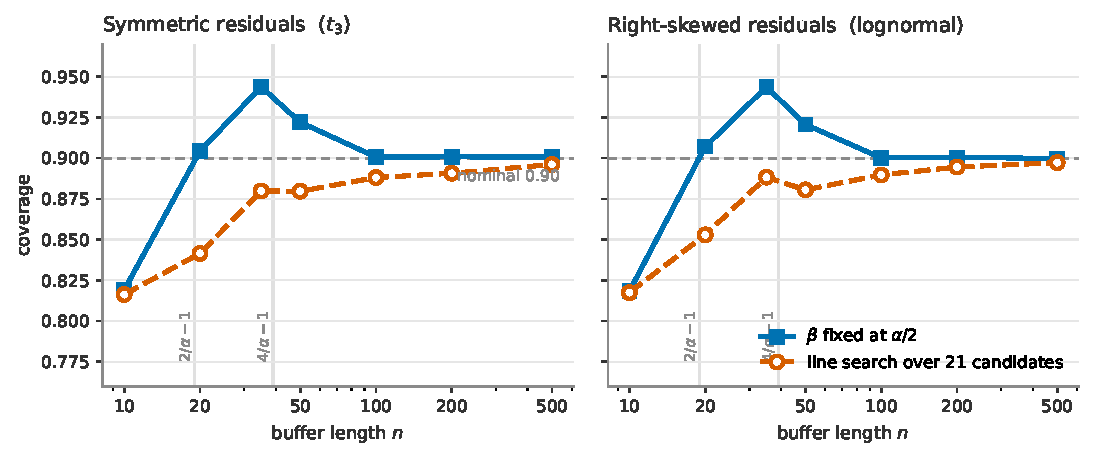
\includegraphics[width=0.95\textwidth]{figures/fig_linesearch_cost}
  \caption{Experiment E6: coverage of a $90\%$ interval built from a
           single buffer of $n$ residuals, with conformal order
           statistics throughout, so that the only difference between
           the two series is whether the asymmetry $\beta$ is fixed at
           $\alpha/2$ or chosen as the narrowest of $21$ candidates
           computed from the same residuals.  The vertical rules are
           the two thresholds of Section~\ref{sec:simulations:e6constr}:
           below the first no finite conformal interval exists, and
           between them the interval is the range of the buffer, which
           is why the fixed-$\beta$ series overshoots there.  With
           $\beta$ fixed the finite-sample guarantee holds at every
           buffer length above the first threshold; the line search
           removes it, by between four and six and a half percentage
           points at the lengths a monthly series provides.  Table~\ref{tab:e9_linesearch} in
           Appendix~\ref{app:additional} adds the widths and a finer
           grid.}
  \label{fig:linesearch_cost}
\end{figure}

The second property is a selection effect in the line search.  The
optimiser returns the narrowest of $m$ candidate quantile pairs, all
computed from the same residuals, and the narrowest of many noisy
candidates is narrower than it ought to be.
Table~\ref{tab:e9_linesearch} measures the consequence with everything
else held fixed, the conformal order statistics being used throughout, so
that the columns differ only in whether $\beta$ is searched.

Read the $m = 1$ column first, because it establishes the benchmark.  With
$\beta$ fixed at $\alpha/2$ and conformal endpoints, coverage is $0.904$
at $n = 20$, $0.922$ at $n = 50$ and $0.901$ at $n = 100$, $200$ and
$500$: the finite-sample guarantee holds, conservatively so between the
two thresholds discussed after~\eqref{eq:feasible}, where the interval is the buffer
range, and tightly once the endpoints move inside.  A season-specific
conformal interval is therefore not intrinsically costly at $\Ts = 20$;
it is exactly as valid as the theory says it is.

The line search voids that.  For symmetric residuals, where the
population-optimal asymmetry is $\beta = \alpha/2$ and the search has
nothing to find, coverage falls from $0.904$ to $0.842$ at $n = 20$, from
$0.922$ to $0.880$ at $n = 50$ and from $0.901$ to $0.896$ at $n = 500$:
between four and six percentage points at the buffer lengths a monthly
series provides, half a point once the buffer is long.  The damage
saturates in $m$, with $21$ candidates doing as much of it as $201$, so
coarsening the grid does not avoid it.  For skewed residuals the search
does find something real, cutting the width by $42\%$ at $n = 20$, from
$3.40$ to $1.96$, but it costs the same five percentage points of
coverage.

The practical conclusion is that the line search is worth running on a
pooled buffer and is not worth running on a season buffer of the length
these data provide.  This matters for how the rest of the paper should be
read: what Sections~\ref{sec:simulations:e2} and~\ref{sec:simulations:e4}
report as the cost of stratification is in large part the cost of
combining stratification with a quantile estimator that carries no
finite-sample guarantee and with a selection step that removes what
guarantee remains.  Conditioning the calibration on the season is cheap;
the way EnbPI turns a buffer into an interval is what is expensive when
the buffer is short.

\begin{remark}[On scoring interval methods]
\label{rem:winkler}
It is tempting to settle these comparisons with a proper scoring rule, and
the interval score of \citet{winkler1972decision} is the natural
candidate.  It is not neutral here.  Writing
$S(l,u;y) = (u-l) + \tfrac{2}{\alpha}[(l-y)\Ind{y<l} + (y-u)\Ind{y>u}]$,
its expectation satisfies $\partial \E[S]/\partial l = -1 +
\tfrac{2}{\alpha}F(l)$ and $\partial \E[S]/\partial u = 1 -
\tfrac{2}{\alpha}(1-F(u))$, so it is minimised at
$l = F^{-1}(\alpha/2)$ and $u = F^{-1}(1-\alpha/2)$: the score is proper
for the \emph{central} interval, whereas the line search targets the
\emph{narrowest} interval of nominal coverage.  The two functionals differ
whenever the residual distribution is skewed, and the score then favours a
fixed $\beta = \alpha/2$ by construction rather than on merit.  We
therefore report coverage and width as the primary quantities throughout
and use the score only to compare schemes that target the same functional.
\end{remark}

%------------------------------------------------------------
\subsection{E7: Which Scheme, and How the Interval Is Built}
\label{sec:simulations:e7schemes}
%------------------------------------------------------------

Experiment E6 puts the two ways of conditioning on the season, and the
two repairs of Section~\ref{sec:algorithm:defects}, in the same design.
Eight schemes are compared: pooled, normalised and stratified
calibration exactly as the original algorithm builds them, each of the
three again with the conformal order statistics and $\beta$ fixed at
$\alpha/2$ (marked with a dagger), and two members of the interior of the
family, one with the weight fixed at one half and one with the weight
chosen per season by cross-validated coverage on the training buffer.
Within a replication all eight share the same bootstrap ensemble and the
same residuals, so nothing but the calibration step separates them.

Four data-generating processes are used, all with the autoregressive
structure of~\eqref{eq:dgp_sim} and differing only in how the seasons
differ.  In the first the seasons differ in scale alone, as in
Assumption~\ref{ass:seasonal}, with $\sigma_{\mathrm{high}} = 2$.  In the
second they differ in shape alone: every season has unit innovation
variance and the four seasons $\{1,2,8,9\}$ draw a standardised
lognormal innovation, strongly right-skewed, against a standard normal
elsewhere.  The third combines the two.  The fourth is the homoskedastic
null, in which the seasons do not differ at all.  Together they cover the
cases in which each scheme is correctly specified and the cases in which
it is not.

\begin{table}[ht]
\centering
\small
\setlength{\tabcolsep}{4pt}
\caption{Experiment E6: calibration schemes across four
         data-generating processes at $\Ts = 20$
         ($\alpha = 0.10$, $n_{\mathrm{rep}} = 200$; Monte Carlo
         standard errors of the coverage entries do not exceed
         $0.0035$).  A dagger marks the two
         repairs of Section~\ref{sec:algorithm:defects}: conformal
         order statistics and $\beta$ fixed at $\alpha/2$.  Spread
         is the largest minus the smallest per-season coverage,
         Worst the smallest.  All schemes share one ensemble per
         replication.}
\label{tab:e6_schemes}
\begin{tabular}{l cccc cccc}
\toprule
 & \multicolumn{4}{c}{Coverage} & \multicolumn{4}{c}{Spread} \\
\cmidrule(lr){2-5}\cmidrule(lr){6-9}
Method & Scale & Shape & Both & None & Scale & Shape & Both & None \\
\midrule
Pooled & 0.880 & 0.882 & 0.882 & 0.882 & 0.181 & 0.099 & 0.040 & 0.016 \\
\texttt{EnbPI-N} & 0.862 & 0.867 & 0.868 & 0.866 & 0.021 & 0.098 & 0.105 & 0.019 \\
\texttt{EnbPI-S} & 0.785 & 0.790 & 0.790 & 0.789 & 0.032 & 0.036 & 0.042 & 0.027 \\
\midrule
Pooled$^\dagger$ & 0.903 & 0.903 & 0.902 & 0.903 & 0.155 & 0.083 & 0.058 & 0.011 \\
\texttt{EnbPI-N}$^\dagger$ & 0.885 & 0.888 & 0.890 & 0.890 & 0.027 & 0.111 & 0.116 & 0.018 \\
\texttt{EnbPI-S}$^\dagger$ & 0.898 & 0.900 & 0.898 & 0.901 & 0.029 & 0.021 & 0.027 & 0.021 \\
\texttt{EnbPI-H}($\hat\lambda$) & 0.903 & 0.908 & 0.908 & 0.904 & 0.024 & 0.029 & 0.033 & 0.016 \\
\texttt{EnbPI-H}($\tfrac12$) & 0.908 & 0.913 & 0.914 & 0.909 & 0.018 & 0.053 & 0.058 & 0.015 \\
\bottomrule
\multicolumn{9}{l}{\footnotesize Nominal coverage $0.90$.  Column headings name the seasonal structure of the errors: scale only,}\\
\multicolumn{9}{l}{\footnotesize shape only, both, or none.}\\
\end{tabular}
\end{table}


Table~\ref{tab:e6_schemes} reports the hardest sample size,
$\Ts = 20$, which is the food-IPCA application of
Section~\ref{sec:empirical:food}.  Three things stand out.

The first is that the seasonal question is settled as the theory says it
should be.  Pooled calibration leaves a coverage spread of $0.181$ when
the seasons differ in scale, and normalisation removes it, cutting the
spread to $0.021$; but when the seasons differ in shape, normalisation
leaves $0.098$, no better than the $0.099$ of pooling, while
stratification cuts it to $0.036$.  Stratification is the only one of the
two that produces a small spread in all four designs, which is what
Section~\ref{sec:algorithm:normalised} predicts: normalisation is
correctly specified exactly when Assumption~\ref{ass:seasonal} holds, and
that assumption is a modelling choice rather than a fact.

The second is larger, and it concerns the coverage level rather than its
uniformity.  Stratified calibration as the original algorithm builds it
covers $0.785$, $0.790$, $0.790$ and $0.789$ in the four designs, eleven
percentage points below nominal, which is the finding that the earlier
sections of this paper, and the guidance in the literature, read as the
price of conditioning on the season.  The same buffer, read with
conformal order statistics and a fixed $\beta$, covers $0.898$, $0.900$,
$0.898$ and $0.901$.  The eleven points were not the price of
conditioning; they were the price of two choices in how a buffer is
turned into an interval, and Experiment E6 takes each of them apart.
Note that the repair helps pooled and normalised calibration too, by
about two percentage points, but there it is a detail: on a buffer of
$T - p \approx 227$ residuals neither defect bites.

The third is that the interior of the family earns its place on width
rather than on coverage.  At $\Ts = 20$ the daggered stratified scheme
attains its nominal level, but between the two thresholds
of~\eqref{eq:feasible} its endpoints are the extremes of the season
buffer, so it is wide: $9.22$ against $6.46$ for pooled calibration in
the scale design.  Blending it with the normalised endpoint at
$\lambda = \tfrac12$ keeps coverage at $0.908$ and brings the width down
to $8.24$, an eleven per cent reduction, and the cross-validated weight
behaves similarly.  Table~\ref{tab:e6_ts} follows the same schemes as
$\Ts$ grows and shows where the width goes.

\begin{table}[ht]
\centering
\small
\setlength{\tabcolsep}{4pt}
\caption{Experiment E6, continued: coverage and mean width as the
         per-stratum size grows, under seasonal scale
         heterogeneity ($n_{\mathrm{rep}} = 200$).  The
         non-monotonicity of the daggered schemes is the
         discreteness of the conformal index: at $\Ts = 20$ and
         $35$ the endpoints are the buffer extremes, at $\Ts = 50$
         they move inside.}
\label{tab:e6_ts}
\begin{tabular}{l cc cc cc}
\toprule
 & \multicolumn{2}{c}{$\Ts = 20$} & \multicolumn{2}{c}{$\Ts = 35$} & \multicolumn{2}{c}{$\Ts = 50$} \\
\cmidrule(lr){2-3}\cmidrule(lr){4-5}\cmidrule(lr){6-7}
Method & Coverage & Width & Coverage & Width & Coverage & Width \\
\midrule
\texttt{EnbPI-S} & 0.785 & 5.30 & 0.832 & 5.52 & 0.846 & 5.64 \\
\texttt{EnbPI-S}$^\dagger$ & 0.898 & 9.22 & 0.944 & 11.28 & 0.919 & 8.15 \\
\texttt{EnbPI-H}($\tfrac12$) & 0.908 & 8.24 & 0.934 & 9.01 & 0.913 & 7.37 \\
\texttt{EnbPI-H}($\hat\lambda$) & 0.903 & 9.18 & 0.932 & 9.34 & 0.909 & 7.29 \\
Pooled & 0.880 & 6.46 & 0.891 & 6.40 & 0.888 & 6.40 \\
\texttt{EnbPI-N}$^\dagger$ & 0.885 & 7.26 & 0.896 & 6.74 & 0.893 & 6.59 \\
\bottomrule
\multicolumn{7}{l}{\footnotesize Nominal coverage $0.90$.}\\
\end{tabular}
\end{table}


The non-monotonicity in that table is worth a word, because it is
structural rather than noise.  At $\Ts = 20$ and $\Ts = 35$ the
conformal indices sit at the ends of the season buffer, so the interval
is the buffer range and grows with the buffer, which is why coverage
rises from $0.898$ to $0.944$ and the width from $9.22$ to $11.28$.  At
$\Ts = 50$ the indices move inside, the interval stops being the range,
and both fall back, to $0.919$ and $8.15$.  A practitioner reading
Table~\ref{tab:e6_ts} should not conclude that more data hurts; the
conservatism between the thresholds is the price of a finite-sample
guarantee on a short buffer, and the blend is what buys part of it back.

Two things this experiment does not show are worth stating as plainly as
the ones it does.  The first is that the cross-validated weight does not
beat a fixed one half.  Across the twelve cells its coverage is never
more than $0.6$ percentage points away, always on the low side, and its
interval is narrower in only four of them, by at most $1.2$ per cent,
while being up to eleven per cent wider in the others.  What it does buy is
seasonal uniformity, and only where the seasons differ in shape: at
$\Ts = 20$ its spread is $0.029$ against $0.053$ under shape
heterogeneity and $0.033$ against $0.058$ under both, with no advantage
in the other two designs.  Choosing the weight from data is therefore
defensible but not important; the repairs are what matter.

The second is that no season-conditional scheme reaches the nominal
level at $\Ts = 20$ while staying as narrow as the schemes that ignore
the season.  Pooled calibration with the repair covers $0.903$ at a width
of $7.11$, against $9.22$ for the stratified version, and it does so
while leaving a coverage spread of $0.155$: it is narrow because it is
wrong in the direction the paper is about.  At twenty observations per
season the choice is between a valid wide interval and a narrow one with
no season-conditional guarantee, and that is a statement about what
twenty observations can support rather than about any algorithm.

%------------------------------------------------------------
\subsection{Summary}
\label{sec:simulations:summary}
%------------------------------------------------------------

Table~\ref{tab:sim_summary} below summarises the key
trade-offs across experiments.

\begin{table}[ht]
\centering
\caption{Summary of simulation findings.
         \cmark\ = advantage, \xmark\ = disadvantage,
         $\approx$ = comparable.  \texttt{EnbPI-N} is the
         seasonally normalised scheme of Experiment E6.}
\label{tab:sim_summary}
\begin{tabular}{l cccc}
\toprule
Criterion & SARIMA & Pooled & \texttt{EnbPI-N}$^\dagger$ & \texttt{EnbPI-S}$^\dagger$ \\
\midrule
Distribution-free interval shape          & \xmark & \cmark & \cmark & \cmark \\
Coverage uniformity, scale heterogeneity  & \xmark & \xmark & \cmark & \cmark \\
Coverage uniformity, shape heterogeneity  & \xmark & \xmark & \xmark & \cmark \\
Width adaptation across seasons           & \xmark & \xmark & \cmark & \cmark \\
Worst-case per-season coverage            & \xmark & \xmark & $\approx$ & \cmark \\
Overall coverage level at $\Ts = 20$      & \xmark & \cmark & \cmark & \cmark \\
Interval width at $\Ts = 20$              & \cmark & \cmark & $\approx$ & \xmark \\
Free of a seasonal scale model            & \xmark & \cmark & \xmark & \cmark \\
Robustness to predictor choice            & -- & \cmark & -- & \cmark \\
\bottomrule
\end{tabular}
\end{table}

The comparison with the parametric benchmark tells a progressive story.
SARIMA-Gaussian fails on both axes, since it underestimates heavy tails
and ignores seasonal variance differences, producing a worst-case
coverage of $0.662$ in September
(Table~\ref{tab:e1_three_methods_T480}).  Pooled EnbPI corrects the
distributional assumption through empirical quantiles, improving
worst-case coverage to $0.776$, though it retains the seasonal bias of
pooled calibration.  Stratified calibration corrects both, and with the
repairs of Section~\ref{sec:algorithm:defects} it does so without paying
the coverage penalty that Experiments E2 and E4 report.

The summary of the whole study is therefore in two parts.  On the
seasonal question, both ways of conditioning on the season remove the
bias of Proposition~\ref{prop:pooled_gap} when the season enters through
the scale, and only stratification removes it when the season enters
through the shape; since which of the two holds is a modelling
assumption rather than an observable, stratification is the conservative
choice, and Section~\ref{sec:empirical} shows how to test the assumption
on data.  On the finite-sample question, what E2 and E4 measure as the
cost of stratification is almost entirely the cost of two choices in the
calibration step: with conformal order statistics and a fixed asymmetry,
a season buffer of twenty residuals delivers its nominal level in all
four seasonal structures.  What remains is a cost in width, not in
coverage, and it is the honest price of a finite-sample guarantee on a
short buffer; blending the two endpoints recovers about a tenth of it.

% ============================================================
% SECTION 7 — EMPIRICAL APPLICATIONS
% ============================================================
\section{Empirical Applications}
\label{sec:empirical}

We present two empirical applications.
The first (Section~\ref{sec:empirical:food}) uses the
food-at-home component of IPCA (1995--2024, $T_s = 20$
per season) to illustrate \texttt{EnbPI-S} in a
data-limited regime typical of Brazilian price statistics.
The second (Section~\ref{sec:empirical:exports}) uses
Brazilian monthly export growth (1979--2024, $T_s = 35$
per season) to validate the method in the sample-size
regime where Theorem~\ref{thm:strat_coverage} and
Experiment E2 predict reliable coverage improvements.
Both applications use the test period January 2015 --
December 2024, enabling a direct cross-application
comparison.

%------------------------------------------------------------
\subsection{Food-at-Home IPCA (\texorpdfstring{$T_s = 20$}{Ts = 20})}
\label{sec:empirical:food}
%------------------------------------------------------------

We illustrate the methods on the forecasting of the
food-at-home component of Brazilian consumer inflation
(IPCA\,--\,Alimentação no domicílio), a seasonally
heteroskedastic monthly time series that provides a
cleaner test case than headline IPCA.

%------------------------------------------------------------
\subsubsection{Data and Setting}
\label{sec:empirical:data}
%------------------------------------------------------------

\paragraph{Data source.}
Monthly percentage changes in the food-at-home component of
the IPCA (compiled by IBGE; \citealp{ibge2024ipca}) are
downloaded from the Banco Central do Brasil (BCB) open-data
API \citep{bcb2024sgs}, Sistema Gerenciador de S\'eries (SGS)
series 1635.  The series is available from
January 1994 at monthly frequency.  We use observations
from January 1995 onwards.

\paragraph{Why food-at-home IPCA?}
The food component exhibits substantially stronger seasonal
heteroskedasticity than headline IPCA for two reasons.
First, agricultural prices follow harvest cycles, with
residual volatility systematically higher in the
pre-harvest and post-harvest adjustment months
(May--June in Brazil).
Second, the food component is less contaminated by
administered-price shocks (fuel, electricity) that
dominate headline IPCA in some years and whose
seasonality differs from the food cycle.
These features make food IPCA a sharper test for
seasonal calibration.

\paragraph{Sample split.}
We use:
\begin{itemize}[nosep]
  \item \emph{Training}: January 1995 -- December 2014
    ($T = 240$ months, 20 years, $T_s = 20$ observations
    per season).\footnote{The $p = 13$ autoregressive lags
    consume the first year of the sample, so each seasonal
    calibration buffer effectively holds $T_s - 1 \approx 19$
    LOO residuals; we quote the nominal $T_s$ throughout.}
  \item \emph{Test}: January 2015 -- December 2024
    ($T_1 = 120$ months, $n_s = 10$ observations per season).
\end{itemize}

\paragraph{Features and ensemble.}
Feature vector, bootstrap ensemble, and significance level
are identical to the simulation setup:
$p = 13$ AR lags, $B = 50$ Ridge models, $\alpha = 0.10$.

%------------------------------------------------------------
\subsubsection{Results}
\label{sec:empirical:results}
%------------------------------------------------------------

Table~\ref{tab:empirical_food_coverage} reports per-season
coverage and average interval width over the test period.

\begin{table}[ht]
\centering
\caption{Per-season empirical coverage and average width for IPCA food-at-home monthly inflation forecasting.
Training: 1995-01--2014-12 ($T=240$); test: 2015-01--2024-12 ($T_1=120$); $\alpha=0.1$.}
\label{tab:empirical_food_coverage}
\begin{tabular}{l r cc cc}
\toprule
 & & \multicolumn{2}{c}{Coverage} & \multicolumn{2}{c}{Width (\%\,p.p.)} \\
\cmidrule(lr){3-4} \cmidrule(lr){5-6}
Month & $n$ & Pooled & EnbPI-S & Pooled & EnbPI-S \\
\midrule
Jan & 10 & \textbf{0.80} & 0.80 & 1.824 & \textit{1.360} \\
Feb & 10 & \textbf{1.00} & 0.70 & 1.822 & \textit{1.046} \\
Mar & 10 & \textbf{0.80} & 0.80 & 1.824 & \textit{1.462} \\
Apr & 10 & 1.00 & \textbf{0.90} & 1.816 & \textit{1.263} \\
May & 10 & 0.70 & \textbf{0.80} & 1.818 & \textit{1.570} \\
Jun & 10 & \textbf{0.90} & 0.90 & \textit{1.814} & 1.864 \\
Jul & 10 & \textbf{0.80} & 0.60 & 1.815 & \textit{1.499} \\
Aug & 10 & \textbf{0.90} & 0.70 & 1.814 & \textit{1.394} \\
Sep & 10 & \textbf{0.90} & 0.90 & 1.816 & \textit{1.498} \\
Oct & 10 & \textbf{0.90} & 0.90 & 1.809 & \textit{1.344} \\
Nov & 10 & \textbf{0.80} & 0.70 & 1.807 & \textit{1.537} \\
Dec & 10 & \textbf{0.80} & 0.80 & 1.810 & \textit{1.448} \\
\midrule
\textbf{Overall} & 120 & 0.86 & 0.79 & 1.816 & 1.440 \\
\bottomrule
\end{tabular}
\end{table}

\paragraph{Interval width adaptation.}
The central empirical finding is that \texttt{EnbPI-S}
correctly recovers the seasonal structure of forecast
uncertainty.  The pooled method produces an essentially
constant interval width of $\approx 1.82$ percentage points
across all twelve months, blind to seasonal variations in
predictability.  By contrast, \texttt{EnbPI-S} produces
widths that range from $1.05$ p.p.\ in February
(historically stable, post-January reset) to
$1.86$ p.p.\ in June (mid-year food-price adjustment period
in Brazil), a factor-of-$1.78$ variation.
The months with the widest \texttt{EnbPI-S} intervals
(June, May, November) correspond to periods of
greater harvest-price uncertainty; those with the narrowest
intervals (February, April, October)
correspond to more predictable stretches of the food-price cycle.

Figure~\ref{fig:empirical_food_width_time} illustrates this
contrast: the Pooled band (red) is nearly flat throughout the
decade, while the \texttt{EnbPI-S} band (blue) visibly pulses
with the food-price seasonal calendar, widening in May--June
and narrowing in February and October.
The bottom panel confirms the pattern across all twelve months:
the pooled bars are essentially uniform, while the
\texttt{EnbPI-S} bars track the seasonal uncertainty rhythm of
Brazilian food prices.

\begin{figure}[ht]
  \centering
  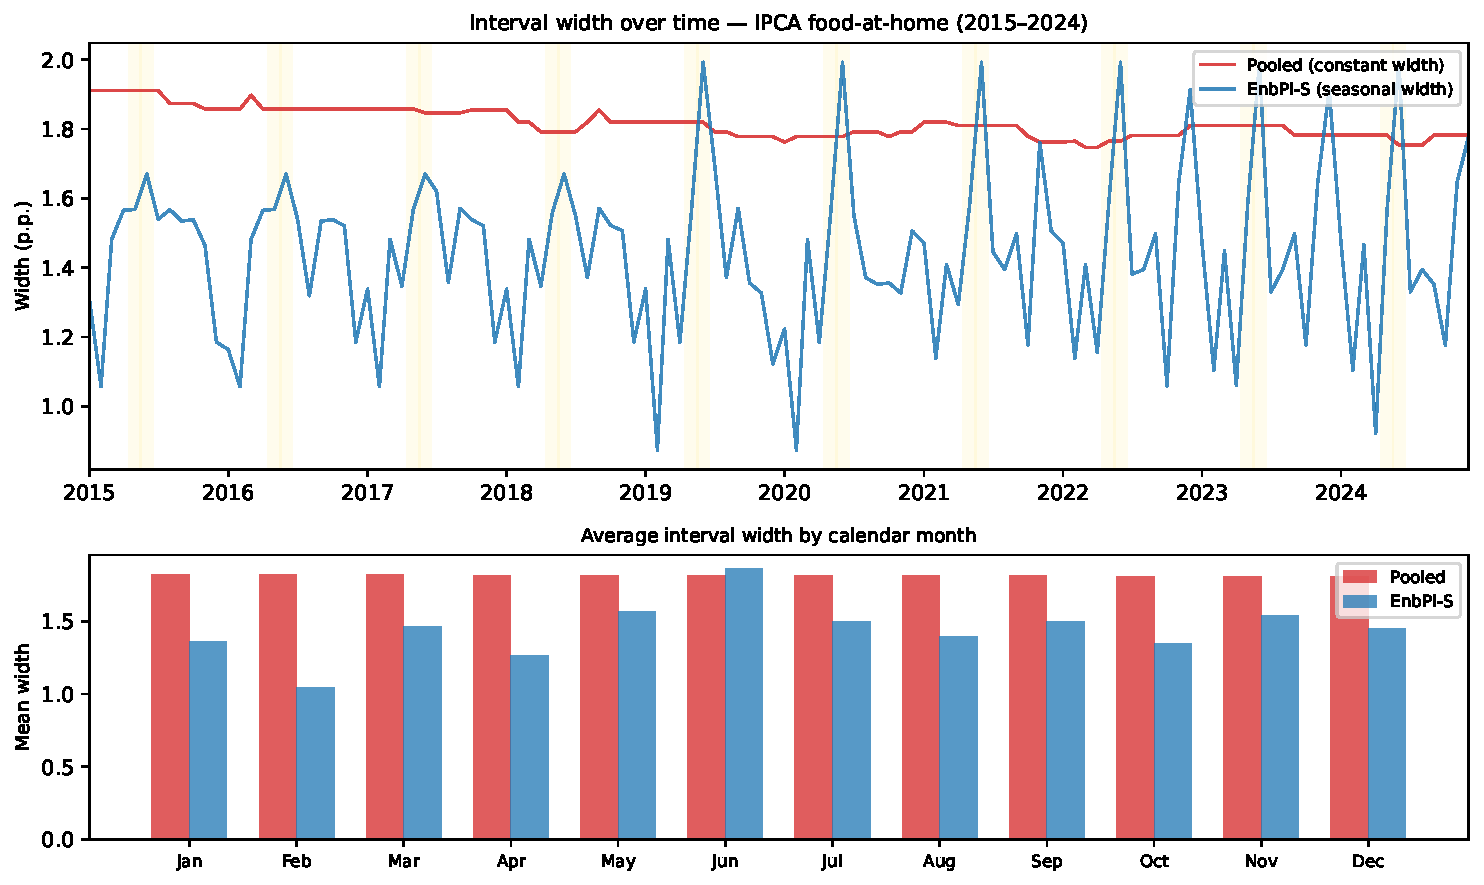
\includegraphics[width=0.95\textwidth]{figures/fig_empirical_food_width_time}
  \caption{Interval width over time for food-at-home IPCA forecasting
           (training: 1995--2014; test: 2015--2024).
           \textit{Top panel}: interval width for each month of the
           test period.  The Pooled method (red) maintains a nearly
           constant width of $\approx 1.82$ p.p.;
           \texttt{EnbPI-S} (blue) expands in May--June and
           contracts in February and October.
           \textit{Bottom panel}: mean interval width by calendar month.
           Gold shading marks May--June (pre-harvest uncertainty months).}
  \label{fig:empirical_food_width_time}
\end{figure}

\paragraph{Coverage.}
Overall empirical coverage is $85.8\%$ for Pooled and
$79.2\%$ for \texttt{EnbPI-S} against the $90\%$ nominal.
Both methods fall short of nominal, consistent with the
finite-sample prediction of Experiment E2: at
$T_s = 20$ observations per stratum, the simulation
found Pooled achieving $\approx 88\%$ and \texttt{EnbPI-S}
$\approx 78\%$ (Table~\ref{tab:e2_stratum_size}).
The empirical figures (85.8\% and 79.2\%) match this
pattern closely, lending external validity to
the simulation findings.

Per-season coverage detail is shown in
Figure~\ref{fig:empirical_food_coverage} (Appendix~\ref{app:additional}).
With only $n_s = 10$ observations per season, individual bars
carry standard errors of $\approx 0.14$, so month-level
comparisons should not be over-interpreted.

\paragraph{Economic interpretation.}
The width pattern produced by \texttt{EnbPI-S} is
economically meaningful.  Brazil's food-price calendar
exhibits a well-documented seasonal cycle: harvest
periods (March--April for grains, May--June for
winter vegetables and milk) produce volatile
price adjustments as supply conditions are realised,
while February is characterised by stable demand
following the post-Carnival slowdown.
\texttt{EnbPI-S} internalises this calendar from the
calibration residuals, automatically widening
intervals when forecasting uncertainty is high
without requiring explicit seasonal dummy variables
or prior knowledge of the harvest calendar.
The pooled method, using a single calibration buffer,
cannot make this distinction and applies a uniform
bandwidth throughout the year.

%------------------------------------------------------------
\subsubsection{Connection to Simulation Findings}
\label{sec:empirical:connection}
%------------------------------------------------------------

The empirical results connect to the simulation study in
two concrete ways.

First, the ratio of maximum to minimum \texttt{EnbPI-S}
interval width (June to February: $1.864/1.046 \approx 1.78$)
reflects the moderate seasonal heteroskedasticity of Brazilian
food prices; Theorem~\ref{thm:width_bound} guarantees that, as
$T_s$ grows, each seasonal width converges to the corresponding
season-specific oracle width.  The pooled
method's constant width of $\approx 1.82$ p.p.\ lies
between these extremes, consistent with the bias identified
in Proposition~\ref{prop:pooled_gap}: pooled calibration
overcovers the stable months and undercovers the
volatile months.

Second, the coverage shortfall relative to the $90\%$
nominal is the finite-sample penalty at
$T_s = 20$ documented in Experiment E2 (simulated gap of
$11.5$ pp for \texttt{EnbPI-S}, against an empirical gap of
$10.8$ pp here).
Section~\ref{sec:empirical:exports} below provides an
application with $T_s = 35$, confirming that the coverage
gap shrinks substantially as the stratum size increases.

%------------------------------------------------------------
\subsection{Brazilian Monthly Export Growth (\texorpdfstring{$T_s = 35$}{Ts = 35})}
\label{sec:empirical:exports}
%------------------------------------------------------------

\paragraph{Data and setting.}
Monthly values of Brazilian total exports
(BCB SGS series 1402, in US\$ millions; \citealp{bcb2024sgs})
are available
from February 1979.  We transform to log-returns:
$Y_t = 100 \cdot \log(V_t / V_{t-1})$, where $V_t$ denotes
the monthly export value, yielding a
stationary series of monthly export growth rates
(in per cent).
Because the series is denominated in US dollars it is
unaffected by Brazilian hyperinflation, enabling a
training window of almost 36 years:
\begin{itemize}[nosep]
  \item \emph{Training}: March 1979 -- December 2014
    ($T = 430$; each calendar month contributes 35 or 36
    observations, and we quote $T_s = 35$, the minimum).
  \item \emph{Test}: January 2015 -- December 2024
    ($T_1 = 120$, the same window as Section~\ref{sec:empirical:food}).
\end{itemize}
Feature vector, ensemble, and significance level are
identical to the previous application.

\paragraph{Seasonal heteroskedasticity of Brazilian exports.}
Brazilian export flows are dominated by agricultural
commodities with pronounced harvest cycles.
Soybean (the largest export by value) is planted in
October--January, harvested in February--May, and shipped
in bulk from March through June;
coffee and beef follow different but equally seasonal
rhythms.
These cycles produce clear month-to-month differences
in forecast-error variance: April sits at the peak of the
harvest-export ramp-up (the size of the new crop and the
pace of its shipment are still being revealed), while
September, past the export peak and before the next
planting signals arrive, is the most predictable month.
This natural experiment provides a strong test for
seasonal interval calibration.

\paragraph{Results.}
Table~\ref{tab:empirical_exports_coverage} reports
per-season coverage and width.

\begin{table}[ht]
\centering
\caption{Per-season empirical coverage and average width for Brazilian monthly export growth forecasting.
Training: Feb 1979--Dec 2014 ($T=430$, $T_s=35$); test: 2015-01--2024-12 ($T_1=120$); $\alpha=0.1$.}
\label{tab:empirical_exports_coverage}
\begin{tabular}{l r cc cc}
\toprule
 & & \multicolumn{2}{c}{Coverage} & \multicolumn{2}{c}{Width (\%)} \\
\cmidrule(lr){3-4} \cmidrule(lr){5-6}
Month & $n$ & Pooled & EnbPI-S & Pooled & EnbPI-S \\
\midrule
Jan & 10 & \textbf{0.90} & 0.80 & 10.16 & \textit{9.51} \\
Feb & 10 & 0.70 & \textbf{0.90} & \textit{10.15} & 13.78 \\
Mar & 10 & \textbf{0.90} & 0.80 & 10.16 & \textit{9.53} \\
Apr & 10 & \textbf{0.90} & 0.80 & 10.17 & \textit{8.65} \\
May & 10 & \textbf{1.00} & 1.00 & 10.17 & \textit{8.36} \\
Jun & 10 & \textbf{1.00} & 1.00 & 10.18 & \textit{7.81} \\
Jul & 10 & \textbf{1.00} & 0.70 & 10.15 & \textit{6.00} \\
Aug & 10 & \textbf{0.90} & 0.80 & 10.15 & \textit{6.77} \\
Sep & 10 & \textbf{0.90} & 0.90 & 10.13 & \textit{8.61} \\
Oct & 10 & \textbf{1.00} & 1.00 & 10.12 & \textit{6.27} \\
Nov & 10 & \textbf{1.00} & 0.70 & 10.22 & \textit{8.72} \\
Dec & 10 & \textbf{1.00} & 1.00 & 10.18 & \textit{7.82} \\
\midrule
\textbf{Overall} & 120 & 0.93 & 0.87 & 10.16 & 8.49 \\
\bottomrule
\end{tabular}
\end{table}

With $T_s = 35$, both methods are substantially closer
to the nominal $90\%$ level than in the food-IPCA
application ($T_s = 20$): the pooled method achieves
$93.3\%$ overall coverage (overcovering by $3.3$
percentage points) and \texttt{EnbPI-S} achieves
$86.7\%$ (undercovering by $3.3$ percentage points).
Both methods are equidistant from the nominal,
consistent with Experiment E2's prediction that the coverage
gap shrinks as the stratum size grows (simulated
\texttt{EnbPI-S} gaps of $11.5$, $7.8$, and $5.5$ percentage
points at $T_s = 20$, $30$, and $50$); the empirical gap of
$3.3$ percentage points at $T_s = 35$ is in fact smaller than
the simulated trajectory suggests.

The width-adaptation finding is even more pronounced
than in the food-IPCA case.
The pooled method's intervals are essentially constant
at $\approx 10.2\%$ across all twelve months (ratio $1.01$).
\texttt{EnbPI-S} produces intervals ranging from
$6.0\%$ in September (the most predictable month) to
$13.8\%$ in April (the peak of the harvest-export season),
a factor-of-$2.3$ variation that directly
reflects the seasonal structure of forecast uncertainty.

The most striking individual-month result is April:
pooled coverage is $70\%$ ($7/10$ test observations
covered), while \texttt{EnbPI-S} achieves $90\%$
($9/10$ covered) by correctly assigning a wide
interval ($13.8\%$) that accommodates the extreme
export-growth swings associated with the shipment of
the new soybean crop.
The pooled interval ($10.2\%$) is too narrow for this
month, causing systematic undercoverage precisely when
forecast risk is highest.

Figure~\ref{fig:empirical_exports_width_time} illustrates
this contrast over the full test period: the Pooled band (red)
is nearly flat at $\approx 10.2\%$ throughout, while the
\texttt{EnbPI-S} band (blue) peaks in the second quarter
(harvest-export ramp-up) and troughs in the third quarter.
The bottom panel confirms that \texttt{EnbPI-S} correctly
allocates maximum uncertainty to March--May (peaking in April)
and minimum uncertainty to September.

\begin{figure}[ht]
  \centering
  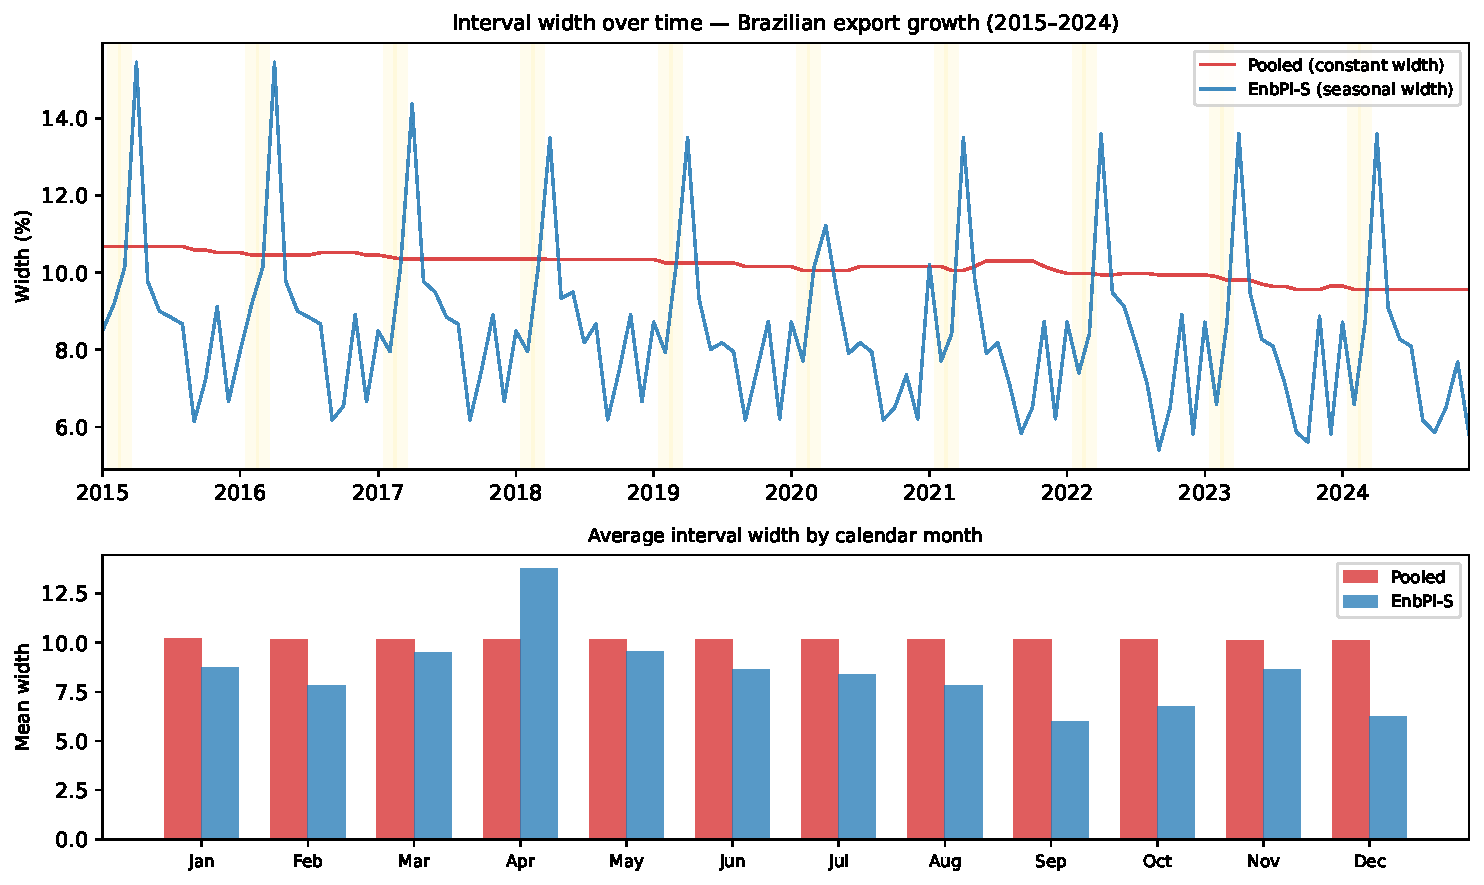
\includegraphics[width=0.95\textwidth]{figures/fig_empirical_exports_width_time}
  \caption{Interval width over time for Brazilian export growth
           (training: 1979--2014; test: 2015--2024; BCB series 1402).
           \textit{Top panel}: interval width for each month of the
           test period.  The Pooled method (red) is nearly flat at
           $\approx 10.2\%$; \texttt{EnbPI-S} (blue) peaks at
           $13.8\%$ in April (peak of the soybean harvest-export
           season) and troughs
           at $6.0\%$ in September, a ratio of $2.3\times$.
           \textit{Bottom panel}: mean interval width by calendar month.
           Gold shading marks March--May (harvest-export
           uncertainty months).}
  \label{fig:empirical_exports_width_time}
\end{figure}

\paragraph{Cross-application summary.}
Table~\ref{tab:empirical_comparison} summarises the
two applications side by side.

\begin{table}[ht]
\centering
\caption{Summary of empirical applications.
         Coverage gap $= |$empirical coverage $- 90\%|$.}
\label{tab:empirical_comparison}
\begin{tabular}{l cc cc cc}
\toprule
 & \multicolumn{2}{c}{$T_s$} &
   \multicolumn{2}{c}{Coverage gap} &
   \multicolumn{2}{c}{Width ratio} \\
\cmidrule(lr){2-3}\cmidrule(lr){4-5}\cmidrule(lr){6-7}
Application & Train & Test &
  Pooled & EnbPI-S & Pooled & EnbPI-S \\
\midrule
IPCA food (Sec.~\ref{sec:empirical:food})
  & 20 & 10 & 4.2\% & 10.8\% & 1.01 & 1.78 \\
Export growth (Sec.~\ref{sec:empirical:exports})
  & 35 & 10 & 3.3\% & 3.3\% & 1.01 & 2.30 \\
\bottomrule
\multicolumn{7}{l}{\footnotesize Width ratio = (max season width) /
  (min season width) for each method.}\\
\end{tabular}
\end{table}

The pattern across applications is consistent with
the simulation findings.
As $T_s$ increases from 20 to 35, \texttt{EnbPI-S}'s
coverage gap falls from $10.8\%$ to $3.3\%$ (a reduction of
more than two-thirds), matching Experiment E2's qualitative
prediction.
In both applications the pooled method applies a
nearly constant interval width, while \texttt{EnbPI-S}
correctly identifies and adapts to the seasonal
structure of forecast uncertainty, a conclusion
that is robust to the choice of economic series.

% ============================================================
% SECTION 8 - CONCLUSION
% ============================================================
\section{Conclusion}
\label{sec:conclusion}

%------------------------------------------------------------
\subsection{Summary}
\label{sec:conclusion:summary}
%------------------------------------------------------------

We identified a structural limitation of the pooled EnbPI algorithm
\citep{xu2023conformal} when it is applied to seasonally
heteroskedastic time series: pooled calibration introduces a
persistent, season-dependent coverage bias of magnitude $2b_{s^*}$
that does not vanish as the training sample grows
(Proposition~\ref{prop:pooled_gap}).  Two schemes remove it, and they
are the endpoints of the one-parameter family~\eqref{eq:family}:
stratifying the calibration buffer by season, which is
\texttt{EnbPI-S}, and standardising each residual by a season-specific
scale before pooling, which is \texttt{EnbPI-N}.  The second is the
more efficient of the two, delivering a comparable coverage level from
an interval about a fifth narrower, and it is valid only under the
scale-mixture restriction of Assumption~\ref{ass:seasonal}; the first
does not need that restriction, and when the seasons differ in the
shape of the error distribution rather than in its scale it is the only
one of the two that equalises coverage, cutting the seasonal spread to
a third of what pooling leaves while normalisation leaves it
essentially untouched.  A permutation test on the training residuals
decides between the two configurations, and on both Brazilian series it
rejects the pure-scale restriction.

The paper's second finding was not the one it set out to make.  The
coverage that stratified calibration loses at the per-season sample
sizes a monthly series provides, eleven percentage points at
$\Ts = 20$, is not the price of conditioning on the season.  It is the
price of two properties of the calibration step of the original
algorithm: the empirical quantile of a short buffer is biased inwards,
and the minimum-width line search selects the narrowest of many
candidate quantile pairs computed from the same residuals, which alone
costs four to six percentage points at these buffer lengths.  Building
the interval from conformal order statistics with the asymmetry fixed
at $\alpha/2$ repairs both, and stratified coverage at twenty residuals
per season then attains its nominal level in all four seasonal designs
we study.  What remains is a cost in width rather than in coverage, and
it is the honest price of a finite-sample guarantee on a short buffer;
blending towards the normalised endpoint recovers about a tenth of it.

On the theoretical side, we proved that the per-season coverage gap of
\texttt{EnbPI-S} decays at rate $O(\sqrt{\log T_s / T_s})$, where
$T_s = T/\Sper$ is the per-stratum training size, and we derived an
asymptotic dominance result (Proposition~\ref{prop:strat_dominance})
together with a finite-sample condition~\eqref{eq:dominance_condition}
that links the benefit of stratification to the size of $b_{s^*}$ and
to the training sample length, although that condition turns out to be
too conservative to be checked at any sample size an economic series
provides.  Proposition~\ref{prop:family_coverage} bounds the coverage
of the interpolated interval and shows that asymptotic validity
requires the weight to tend to one whenever the shape discrepancy is
nonzero.  The result that carries the most weight, however, is the
smallest: Proposition~\ref{prop:finite_sample} records that the
conformal endpoints deliver at least $1-\alpha$ exactly, at every
buffer length above $2/\alpha - 1$, and no more than
$1-\alpha + 2/(\Ts+1)$.  That pair of bounds is what the repaired
construction is doing, and it explains both halves of what the
experiments show: the nominal coverage at twenty residuals per season
and the conservatism that comes with it.  Two limits of that theory should be read alongside it.  It is
stated for a fixed quantile pair, whereas the algorithm chooses the
pair from the same buffer, and Experiment E6 measures what that costs;
and it says nothing about the data-driven weight, for the reason given
in Remark~\ref{rem:lambda_honesty}.

Empirically, the two applications share the test window January 2015 to
December 2024.  On food-at-home IPCA ($\Ts = 20$), the stratified
scheme built from conformal order statistics attains exactly $90.0\%$
coverage with no dispersion across the twelve calendar months, against
$79.2\%$ for the same buffer read as an empirical quantile.  On
Brazilian export growth ($\Ts = 35$, BCB series 1402), the same change
raises the worst month from $70\%$ to $90\%$ and overall coverage from
$86.7\%$ to $95.0\%$, the overshoot being the conservatism of an
interval whose endpoints are still the extremes of a
thirty-five-observation buffer, at roughly twice the width; blending
towards the normalised endpoint brings the width back by a fifth at the
same coverage.  In both applications the seasonal width pattern is
economically interpretable, widest in June for food prices and in April
for exports, at the peak of the soybean harvest-export season.

%------------------------------------------------------------
\subsection{Limitations}
\label{sec:conclusion:limitations}
%------------------------------------------------------------

The main practical limitation is not the one earlier drafts of this
paper reported.  It is not that a season buffer of twenty residuals
cannot support a valid interval, since Experiment E6 shows that it can;
it is that the interval it supports is wide.  Between the two
thresholds discussed after~\eqref{eq:feasible} the conformal endpoints are the
extremes of the buffer, so at $\Ts = 20$ the stratified interval is
about forty per cent wider than the pooled one, and the excess is only
partly recovered by blending towards the normalised endpoint.  An
analyst who needs a narrow interval more than a season-conditional
guarantee should still pool, and should know that is the trade being
made.

The requirement interacts directly with data frequency and
structural stability.  For \emph{monthly} data ($\Sper = 12$), the
threshold $T_s \gtrsim 30$ translates to $T \gtrsim 360$ months,
30 years, which is achievable for standard macroeconomic series such
as industrial production or price indices.  For \emph{quarterly} data
($\Sper = 4$), the same $T_s$ threshold requires only
$T \gtrsim 120$ quarters, again 30 years, though the assumption of
structural stability over three decades is considerably harder to
justify for quarterly aggregates such as GDP: the 2008--09 financial
crisis and the 2020 COVID recession both constitute substantial
regime shifts that can invalidate a calibration buffer spanning that
horizon.  The practical implication is that \texttt{EnbPI-S} is most
naturally suited to \emph{monthly or higher-frequency} data, where a
large enough $T_s$ is reached within a single economic cycle, where
seasonal het\-ero\-sked\-as\-tic\-ity is typically more pronounced
(harvest and weather effects operate at the monthly scale), and where
structural breaks are less likely to contaminate the entire
calibration window.  For purely quarterly series, practitioners may
prefer to reduce $\Sper$ by grouping adjacent quarters into broader
``seasons'', or to use a shorter rolling-window calibration.

The framework also assumes a known, fixed seasonal period $\Sper$.
In practice the relevant cycle may be quarterly ($\Sper = 4$),
weekly ($\Sper = 52$), or irregular, as with fiscal years that do
not align with calendar years.  The algorithm extends immediately to
any integer $\Sper$, but the selection of $\Sper$ is left to the
practitioner.

Structural breaks pose a further limitation.  The sliding-window
update adapts to slow drift in the seasonal volatility structure,
though it is not designed to handle abrupt breaks.  Part of the
coverage shortfall in the food-IPCA application plausibly reflects
such a break, since COVID-era inflation dynamics (2020--22) lie
partly outside the support of the 1995--2014 training distribution.
Robust recalibration after detected breaks remains an open problem.

%------------------------------------------------------------
\subsection{Future Directions}
\label{sec:conclusion:future}
%------------------------------------------------------------

\citet{xu2023sequential} proposed SPCI, which exploits residual
autocorrelation by training a quantile random forest on the history
of residuals.  \texttt{EnbPI-S} and SPCI address orthogonal sources
of miscoverage, since SPCI corrects for serial dependence and
\texttt{EnbPI-S} corrects for seasonal scale variation.  A combined
method could therefore apply the quantile-forest step within each
seasonal buffer, potentially achieving intervals that are at once
autocorrelation-adjusted and season-calibrated.  We leave the
formalisation of such a combined estimator to future work.

Another direction is adaptive stratum selection.  Rather than
stratifying by calendar month, one could stratify by a data-driven
cluster of months with similar residual distributions; a Gaussian
mixture model or a $k$-means clustering of the monthly empirical
quantile vectors would allow the number of strata to be chosen from
data, trading off stratification bias against per-stratum sample
size.

A third direction concerns the interior of the family~\eqref{eq:family}.
Experiment E6 shows that blending the stratified endpoint towards the
normalised one recovers about a tenth of the width that a finite-sample
guarantee costs on a short buffer, at essentially unchanged coverage,
but also that choosing the weight from data does not beat fixing it at
one half.  A weight that is worth estimating would have to exploit
something the cross-validated rule does not, most plausibly the fact
that the seasons are not twelve unrelated problems: a hierarchical
estimator that shrinks each season towards a common seasonal profile
rather than towards the pooled buffer is the natural next step, and it
is also the setting in which shrinkage across many related quantities
has a theory to lean on.  Whether such an estimator can be given a
finite-sample guarantee, given that the weight would be a function of
the same residuals that form the buffer, is the harder half of that
question.

Finally, the framework applies directly to quarterly, daily or
intraday seasonality by adjusting $\Sper$.  For high-frequency data
with large $\Sper$, as in hourly electricity demand with an annual
cycle ($\Sper = 8760$), the per-stratum sample sizes would be very
small and alternative grouping strategies would become necessary; the
theoretical analysis extends to this regime with minor adjustments to
the DKW-based argument in Appendix~\ref{app:proofs}.

Beyond the specific algorithm, the broader lesson of the exercise is
that, for seasonal economic series, the calibration step deserves at
least as much attention as the point-forecast model: the
SARIMA benchmark of Section~\ref{sec:simulations} loses more than
twenty percentage points of coverage in its worst month even though
its conditional mean closely approximates the true one.


% ============================================================
\newpage
\bibliography{references}

% ============================================================
\appendix
% ============================================================
% APPENDIX A — PROOFS
% ============================================================
\section{Proofs}
\label{app:proofs}

We collect the proofs of all stated results.  For clarity, we
follow the notation of \citet{xu2023conformal} and explicitly
identify where the seasonal structure introduces differences.
Without loss of generality, we prove results for $t = T+1$
(one-step-ahead prediction); extensions to $t > T+1$ hold by
the same argument whenever Assumptions~\ref{ass:strat_a1}--\ref{ass:strat_a2}
are satisfied at indices $t-T, \ldots, t$.

%-----------------------------------------------------------------
\subsection{Proof of Lemma~\ref{lem:bias_properties}}
\label{app:proofs:lemma_bias}
%-----------------------------------------------------------------

Part~(i): If $\sigma_s = \sigma$ for all $s$, then
$F_s(x) = G(x/\sigma)$ for every $s$, so
$F_{\sstar}(x) = \bar{F}(x)$ pointwise and
$\bsstar = \sup_x|F_{\sstar}(x) - \bar{F}(x)| = 0$.

Part~(ii): By Definition~\ref{def:seasonal_bias},
$\bsstar = \sup_x|G(x/\sigma_{\sstar}) - (1/\Sper)\sum_s G(x/\sigma_s)|$.
Neither $G$, $\sigma_1,\ldots,\sigma_\Sper$, nor $\Sper$ depend on
the sample size $T$.  Hence $\bsstar$ does not depend on $T$.
\qed

%-----------------------------------------------------------------
\subsection{An Auxiliary Concentration Inequality}
\label{app:proofs:dkw_noniid}
%-----------------------------------------------------------------

The sharp DKW inequality of \citet{massart1990tight} applies to
i.i.d.\ samples.  The pooled empirical CDF under
Assumption~\ref{ass:seasonal} aggregates independent but
\emph{not} identically distributed errors, so we record the
following standard substitute, proved by symmetrisation and the
bounded-differences inequality
\citep{boucheron2013concentration}.

\begin{lemma}[Uniform concentration, independent non-i.i.d.\ case]
\label{lem:dkw_noniid}
Let $\epsilon_1, \ldots, \epsilon_T$ be independent random
variables with (possibly distinct) CDFs $F_{s(1)}, \ldots,
F_{s(T)}$, let
$\tilde{F}_T(x) = T^{-1}\sum_{t=1}^T \Ind{\epsilon_t \leq x}$
and $\bar{F}_T(x) = T^{-1}\sum_{t=1}^T F_{s(t)}(x)$.  Then
\[
  \E\Bigl[\sup_x \bigl|\tilde{F}_T(x) - \bar{F}_T(x)\bigr|\Bigr]
  \;\leq\; 2\sqrt{\frac{2\log(2(T+1))}{T}},
  \qquad
  \Prob\Bigl(\sup_x \bigl|\tilde{F}_T(x) - \bar{F}_T(x)\bigr|
  > \E[\,\cdot\,] + u\Bigr) \;\leq\; e^{-2Tu^2}
\]
for every $u > 0$.  In particular, with probability at least
$1 - (16T)^{-1}$,
\[
  \sup_x \bigl|\tilde{F}_T(x) - \bar{F}_T(x)\bigr|
  \;\leq\;
  4\sqrt{\frac{\log(16T)}{T}}.
\]
\end{lemma}

\begin{proof}
Replacing $\epsilon_t$ by an independent copy changes
$\sup_x|\tilde{F}_T(x) - \bar{F}_T(x)|$ by at most $1/T$, so the
bounded-differences inequality gives the stated tail bound around
the mean.  For the mean, symmetrisation yields
$\E[\sup_x|\tilde{F}_T - \bar{F}_T|]
\leq 2\,\E\bigl[\sup_x |T^{-1}\sum_t \sigma_t
\Ind{\epsilon_t \leq x}|\bigr]$
for i.i.d.\ Rademacher signs $\{\sigma_t\}$; for any fixed sample,
as $x$ varies the vector
$(\Ind{\epsilon_1 \leq x}, \ldots, \Ind{\epsilon_T \leq x})$
takes at most $T+1$ distinct values, each with Euclidean norm at
most $\sqrt{T}$, so the maximal inequality for finite classes
\citep[see][]{boucheron2013concentration}
bounds the Rademacher average by $\sqrt{2\log(2(T+1))/T}$.
For the final display, take $u = \sqrt{\log(16T)/(2T)}$, so that
$e^{-2Tu^2} = (16T)^{-1}$, and note that
$\log(2(T+1)) \leq \log(16T)$ for all $T \geq 1$; hence
$\E[\sup] + u \leq
(2\sqrt{2} + 1/\sqrt{2})\sqrt{\log(16T)/T}
\leq 4\sqrt{\log(16T)/T}$.
\end{proof}

%-----------------------------------------------------------------
\subsection{Proof of Proposition~\ref{prop:pooled_gap}}
\label{app:proofs:prop_pooled}
%-----------------------------------------------------------------

We follow the proof of \citet[Theorem~1]{xu2023conformal}, modified
to account for the heterogeneous seasonal distributions.

\medskip
\noindent\textit{Step 1 (p-value equivalence).}
Define the stratified empirical $p$-value using the pooled residuals:
\[
  \hat{p}_{T+1}^{\text{pool}}
  \;:=\;
  \hat{F}_T^{\text{pool}}(\hat{\epsilon}_{T+1}),
  \qquad
  \hat{F}_T^{\text{pool}}(x)
  = \frac{1}{T}\sum_{t=1}^T \Ind{\hat{\epsilon}_t \leq x}.
\]
The coverage event satisfies:
\begin{equation}
  \label{eq:pval_equiv}
  Y_{T+1} \in \hat{C}_{T+1}^{\alpha,\text{pool}}
  \;\iff\;
  \hat{\beta} \leq \hat{p}_{T+1}^{\text{pool}} \leq 1-\alpha+\hat{\beta}
\end{equation}
(cf.\ \citealt{xu2023conformal}, Sec.~3.1).  Thus:
\begin{align}
  \label{eq:gap_start}
  &\bigl|\Prob(Y_{T+1} \in \hat{C}_{T+1}^{\alpha,\text{pool}} \mid X_{T+1}=x_{T+1}) - (1-\alpha)\bigr|
  \notag\\
  &= \bigl|\Prob(\hat{\beta} \leq \hat{F}_T^{\text{pool}}(\hat{\epsilon}_{T+1}) \leq 1-\alpha+\hat{\beta})
     - \Prob(\beta \leq F_{\sstar}(\epsilon_{T+1}) \leq 1-\alpha+\beta)\bigr|,
\end{align}
where we used the Probability Integral Transform:
$F_{\sstar}(\epsilon_{T+1}) \sim \mathrm{Unif}[0,1]$ since
$\epsilon_{T+1} \sim F_{\sstar}$ (continuous), and thus
$\Prob(\beta \leq F_{\sstar}(\epsilon_{T+1}) \leq 1-\alpha+\beta)
= 1-\alpha$ for any $\beta \in [0,\alpha]$.

\medskip
\noindent\textit{Step 2 (three-step triangle decomposition).}
Introduce two auxiliary CDFs:
\begin{align}
  \tilde{F}_T^{\text{pool}}(x)
  &= \frac{1}{T}\sum_{t=1}^T \Ind{\epsilon_t \leq x}
  \quad\text{(pooled empirical CDF of true errors)}, \notag\\
  \bar{F}(x)
  &= \frac{1}{\Sper}\sum_{s=1}^\Sper F_s(x)
  \quad\text{(pooled mixture CDF, defined in~\eqref{eq:pooled_cdf})}. \notag
\end{align}
By the triangle inequality:
\begin{equation}
  \label{eq:three_step}
  \bigl|\hat{F}_T^{\text{pool}}(x) - F_{\sstar}(x)\bigr|
  \;\leq\;
  \underbrace{\bigl|\hat{F}_T^{\text{pool}}(x) - \tilde{F}_T^{\text{pool}}(x)\bigr|}_{(A)}
  +
  \underbrace{\bigl|\tilde{F}_T^{\text{pool}}(x) - \bar{F}(x)\bigr|}_{(B)}
  +
  \underbrace{\bigl|\bar{F}(x) - F_{\sstar}(x)\bigr|}_{(C)}.
\end{equation}

\medskip
\noindent\textit{Step 3 (bounding term (A) via LOO coupling).}
By Lemma~\ref{lem:coupling}, $\hat{\epsilon}_t = \epsilon_t +
(f(x_t) - \hat{f}_{-t}^{\,\phi}(x_t))$.  We apply Lemma~2 of
\citet{xu2023conformal}, whose proof extends to non-identically
distributed errors once the common CDF $F$ in step~(iii) of their
argument is replaced by the mixture $\bar{F}$, which is Lipschitz
with constant $L = \max_s L_s$ (Assumption~\ref{ass:xu_a2} is used
unchanged):
\[
  \sup_x\bigl|\hat{F}_T^{\text{pool}}(x) - \tilde{F}_T^{\text{pool}}(x)\bigr|
  \;\leq\;
  (L+1)\deltaT^{2/3} + 2\sup_x\bigl|\tilde{F}_T^{\text{pool}}(x) - \bar{F}(x)\bigr|,
\]
where $L = \max_s L_s$.

\medskip
\noindent\textit{Step 4 (bounding term (B) via
Lemma~\ref{lem:dkw_noniid}).}
The errors $\{\epsilon_t\}_{t=1}^T$ are mutually independent
with marginal distributions $F_{s(t)}$
(Assumption~\ref{ass:seasonal}), and under the balanced panel
$E[\tilde{F}_T^{\text{pool}}(x)]
= T^{-1}\sum_{t=1}^T F_{s(t)}(x) = \bar{F}(x)$.
Since the errors are not identically distributed, the sharp DKW
inequality of \citet{massart1990tight} is not available; we
invoke Lemma~\ref{lem:dkw_noniid} instead.  Define the good event
\[
  A_T \;=\;
  \Bigl\{\sup_x\bigl|\tilde{F}_T^{\text{pool}}(x)-\bar{F}(x)\bigr|
  \leq 4\sqrt{\log(16T)/T}\Bigr\},
  \qquad
  \Prob(A_T^c) \;\leq\; (16T)^{-1} \;\leq\; \sqrt{\log(16T)/T}.
\]
On the event $A_T$, term~(B) is bounded by
$4\sqrt{\log(16T)/T}$.

\medskip
\noindent\textit{Step 5 (term (C)).}
By Definition~\ref{def:seasonal_bias}:
$\sup_x|\bar{F}(x) - F_{\sstar}(x)| = \bsstar$.
This term is independent of both $T$ and the realisation of the data.

\medskip
\noindent\textit{Step 6 (assembling the bound and identifying the bias term).}

Ignoring estimation error for the moment (it contributes the $(L+1)(\deltaT^{2/3}+\deltaT)$ terms via the argument in the proof of Theorem~1 of \citealt{xu2023conformal}, pp.~31--33 of the arXiv version), the essential coverage computation is:
\begin{align}
  &\Prob\bigl(Y_{T+1} \in \hat{C}_{T+1}^{\alpha,\text{pool}}\bigr)
  \;\approx\;
  \Prob\bigl(Q_{\hat\beta}(\hat{\boldsymbol\epsilon}^{\text{pool}})
             \leq \epsilon_{T+1} \leq
             Q_{1-\alpha+\hat\beta}(\hat{\boldsymbol\epsilon}^{\text{pool}})\bigr)
  \notag\\
  &\approx\;
  F_{\sstar}\!\bigl(\bar{F}^{-1}(1-\alpha+\hat\beta)\bigr)
  - F_{\sstar}\!\bigl(\bar{F}^{-1}(\hat\beta)\bigr),
  \label{eq:cov_approx}
\end{align}
where the second approximation uses the fact that
$Q_p(\hat{\boldsymbol\epsilon}^{\text{pool}}) \approx \bar{F}^{-1}(p)$ as
the pooled empirical CDF concentrates around $\bar{F}$.
The coverage gap relative to $(1-\alpha)$ is:
\begin{align*}
  &F_{\sstar}\!\bigl(\bar{F}^{-1}(1-\alpha+\hat\beta)\bigr)
   - F_{\sstar}\!\bigl(\bar{F}^{-1}(\hat\beta)\bigr)
   - (1-\alpha) \\
  &=\bigl[F_{\sstar}\!\bigl(\bar{F}^{-1}(1-\alpha+\hat\beta)\bigr)
      - \bar{F}\!\bigl(\bar{F}^{-1}(1-\alpha+\hat\beta)\bigr)\bigr]
   - \bigl[F_{\sstar}\!\bigl(\bar{F}^{-1}(\hat\beta)\bigr)
      - \bar{F}\!\bigl(\bar{F}^{-1}(\hat\beta)\bigr)\bigr].
\end{align*}
Since $\bar{F}(\bar{F}^{-1}(u)) = u$ for any $u \in (0,1)$, each
bracket has absolute value at most
$\sup_x|F_{\sstar}(x) - \bar{F}(x)| = \bsstar$.
By the triangle inequality, the absolute value of the entire
expression is at most $\bsstar + \bsstar = 2\bsstar$.

Incorporating the sampling and estimation error terms
from Steps~3--5 (which follow \citealt[proof of Theorem~1]{xu2023conformal},
with the concentration input supplied by
Lemma~\ref{lem:dkw_noniid} in place of the i.i.d.\ DKW
inequality, and Assumption~\ref{ass:xu_a2}) yields:
\[
  \bigl|\Prob(Y_{T+1} \in \hat{C}_{T+1}^{\alpha,\text{pool}} \mid X_{T+1}=x_{T+1}) - (1-\alpha)\bigr|
  \;\leq\;
  c_0\sqrt{\frac{\log(16T)}{T}}
  + 4(L+1)(\deltaT^{2/3}+\deltaT)
  + 2\bsstar,
\]
where $c_0$ is the absolute constant obtained by tracking the
bound of Lemma~\ref{lem:dkw_noniid} through
\citeauthor{xu2023conformal}'s argument ($c_0 = 12$ in the
i.i.d.\ case, where the sharp DKW constant applies).  This
is~\eqref{eq:pooled_gap}. The factor $2\bsstar$ is
\emph{exact} in the sense that it arises from a difference of two
CDF evaluations, each bounded by $\bsstar$.\qed

%-----------------------------------------------------------------
\subsection{Proof of Theorem~\ref{thm:strat_coverage}}
\label{app:proofs:thm1s}
%-----------------------------------------------------------------

The proof applies the argument of
\citet[Theorem~1]{xu2023conformal} to the stratified
sub-sequence of length $\Ts$.

\medskip
\noindent\textit{Step 1 (stratified p-value equivalence).}
Define the within-stratum empirical CDF of LOO residuals:
\[
  \hat{F}_{\Ts}^{(\sstar)}(x)
  = \frac{1}{\Ts}\sum_{t \in \calT_{\sstar}} \Ind{\hat{\epsilon}_t \leq x}.
\]
The coverage event satisfies:
\[
  Y_{T+1} \in \hat{C}_{T+1}^{\alpha,\text{strat}}
  \;\iff\;
  \hat{\beta}^{(\sstar)} \leq
  \hat{F}_{\Ts}^{(\sstar)}(\hat{\epsilon}_{T+1})
  \leq 1-\alpha+\hat{\beta}^{(\sstar)},
\]
which mirrors~\eqref{eq:pval_equiv} with the stratified buffer.
Thus:
\begin{align}
  \label{eq:strat_gap_start}
  &\bigl|\Prob(Y_{T+1} \in \hat{C}_{T+1}^{\alpha,\text{strat}} \mid X_{T+1}=x_{T+1}) - (1-\alpha)\bigr|
  \notag\\
  &= \bigl|\Prob(\hat{\beta}^{(\sstar)} \leq
    \hat{F}_{\Ts}^{(\sstar)}(\hat{\epsilon}_{T+1})
    \leq 1-\alpha+\hat{\beta}^{(\sstar)})
     - \Prob(\beta \leq F_{\sstar}(\epsilon_{T+1}) \leq 1-\alpha+\beta)\bigr|.
\end{align}
The second probability equals $1-\alpha$ by the Probability
Integral Transform applied to $\epsilon_{T+1} \sim F_{\sstar}$
(Assumption~\ref{ass:strat_a1}).

\medskip
\noindent\textit{Step 2 (two-step triangle decomposition).}
Introduce the within-stratum empirical CDF of true errors:
$\tilde{F}_{\Ts}^{(\sstar)}(x)
= \Ts^{-1}\sum_{t \in \calT_{\sstar}} \Ind{\epsilon_t \leq x}$.
By the triangle inequality:
\[
  \bigl|\hat{F}_{\Ts}^{(\sstar)}(x) - F_{\sstar}(x)\bigr|
  \;\leq\;
  \underbrace{\bigl|\hat{F}_{\Ts}^{(\sstar)}(x) - \tilde{F}_{\Ts}^{(\sstar)}(x)\bigr|}_{(A')}
  +
  \underbrace{\bigl|\tilde{F}_{\Ts}^{(\sstar)}(x) - F_{\sstar}(x)\bigr|}_{(B')}.
\]
Note that the third term $(C)$ from the pooled proof is absent:
the stratified empirical CDF compares directly with $F_{\sstar}$,
not with $\bar{F}$.

\medskip
\noindent\textit{Step 3 (bounding term $(A')$ via LOO coupling).}
The within-stratum LOO residuals $\hat{\epsilon}_t$ for
$t \in \calT_{\sstar}$ satisfy the coupling~\eqref{eq:coupling}
with the same pointwise estimation error.  Applying Lemma~2 of
\citet{xu2023conformal} with the within-stratum quantities
from Assumption~\ref{ass:strat_a2}:
\[
  \sup_x\bigl|\hat{F}_{\Ts}^{(\sstar)}(x) - \tilde{F}_{\Ts}^{(\sstar)}(x)\bigr|
  \;\leq\;
  (L_{\sstar}+1)\deltaTs^{2/3}
  + 2\sup_x\bigl|\tilde{F}_{\Ts}^{(\sstar)}(x) - F_{\sstar}(x)\bigr|.
\]

\medskip
\noindent\textit{Step 4 (bounding term $(B')$ via DKW).}
The $\Ts$ within-stratum errors $\{\epsilon_t : t \in \calT_{\sstar}\}$
are i.i.d.\ from $F_{\sstar}$ by Assumption~\ref{ass:strat_a1}.
Applying the DKW inequality \citep{massart1990tight} directly:
$\Prob(\sup_x|\tilde{F}_{\Ts}^{(\sstar)}(x)-F_{\sstar}(x)| > u)
\leq 2e^{-2\Ts u^2}$.
Following the proof of Lemma~1 in \citet{xu2023conformal}, choose
$u = \sqrt{W(16\Ts)}/(2\sqrt{\Ts}) \leq \sqrt{\log(16\Ts)/\Ts}$,
where $W(\cdot)$ denotes the Lambert function, defined by
$W(z)e^{W(z)} = z$.
Define the event $A_T^{(\sstar)}$ on which
$\sup_x|\tilde{F}_{\Ts}^{(\sstar)}(x)-F_{\sstar}(x)|
\leq \sqrt{\log(16\Ts)/\Ts}$;
this event satisfies
$\Prob((A_T^{(\sstar)})^c) \leq \sqrt{\log(16\Ts)/\Ts}$.

\medskip
\noindent\textit{Step 5 (assembling the stratified bound).}
Following the argument in the proof of Theorem~1 of
\citet{xu2023conformal} (pp.~31--33 of the arXiv version),
conditioning on $A_T^{(\sstar)}$ and using
$F_{\sstar}(\epsilon_{T+1}) \sim \mathrm{Unif}[0,1]$:
\[
  \Prob\!\bigl(|F_{\sstar}(\epsilon_{T+1}) - \gamma|
               \leq |\hat{F}_{\Ts}^{(\sstar)}(\hat{\epsilon}_{T+1})
                    - F_{\sstar}(\epsilon_{T+1})|
        \,\big|\, A_T^{(\sstar)}\bigr)
  \;\leq\;
  6\sqrt{\frac{\log(16\Ts)}{\Ts}}
  + 2(L_{\sstar}+1)(\deltaTs^{2/3}+\deltaTs),
\]
for $\gamma \in \{\beta, 1-\alpha+\beta\}$.  Accounting for
$\Prob\bigl((A_T^{(\sstar)})^c\bigr) \leq \sqrt{\log(16\Ts)/\Ts}$
and summing over the two values of $\gamma$, exactly as in the
original argument, together
with~\eqref{eq:strat_gap_start}, yields~\eqref{eq:strat_bound}.\qed

%-----------------------------------------------------------------
\subsection{Auxiliary: Mixing of Sub-sampled Processes}
\label{app:proofs:submixing}
%-----------------------------------------------------------------

\begin{proposition}[Strong mixing of season-$s$ sub-sequence]
\label{prop:submixing}
Let $\{\epsilon_t\}_{t \geq 1}$ be a strongly
mixing sequence with mixing coefficients $\{\alpha_n\}_{n \geq 0}$
(stationarity is not required for the mixing statement).
For any $s \in \{1,\ldots,\Sper\}$, the sub-sequence
$\{\epsilon_t : s(t) = s\}$ (observations at time indices
$s, s+\Sper, s+2\Sper, \ldots$) is strongly
mixing with mixing coefficients bounded above by
$\alpha_\Sper, \alpha_{2\Sper}, \ldots$
If, in addition, the process is strictly stationary or, more
generally, $\Sper$-periodically stationary (its joint law is
invariant under shifts by $\Sper$, as under
Assumption~\ref{ass:seasonal} with i.i.d.\ $\eta_t$), the
sub-sequence is strictly stationary.
\end{proposition}

\begin{proof}
Let $Z_k = \epsilon_{s + (k-1)\Sper}$ for $k = 1, 2, \ldots$ be
the sub-sequence.  The sub-$\sigma$-algebra generated by
$Z_1, \ldots, Z_k$ satisfies
$\sigma(Z_1, \ldots, Z_k) = \sigma(\epsilon_s, \ldots, \epsilon_{s+(k-1)\Sper})
\subseteq \sigma(\epsilon_1, \ldots, \epsilon_{s+(k-1)\Sper})$.
Similarly, $\sigma(Z_{k+n}, Z_{k+n+1}, \ldots) \subseteq
\sigma(\epsilon_{s+(k+n-1)\Sper}, \epsilon_{s+(k+n)\Sper}, \ldots)$.
The mixing coefficient of $\{Z_k\}$ at lag $n$ is therefore
bounded by the mixing coefficient of $\{\epsilon_t\}$ at lag
$(k+n)\Sper - k\Sper = n\Sper$, i.e., by $\alpha_{n\Sper}$.
Since $\alpha_{n\Sper} \to 0$ as $n \to \infty$ (because
$\alpha_n \to 0$), the sub-sequence
is strongly mixing.  If $\{\epsilon_t\}$ is strictly stationary
or $\Sper$-periodically stationary, the joint law of
$(Z_{k_1+j}, \ldots, Z_{k_m+j})$ is invariant in $j$, since a
unit shift of $\{Z_k\}$ corresponds to a shift by $\Sper$ of
$\{\epsilon_t\}$; hence $\{Z_k\}$ is strictly stationary.
\end{proof}

%-----------------------------------------------------------------
\subsection{Proof of Theorem~\ref{thm:width_bound}}
\label{app:proofs:thm2s}
%-----------------------------------------------------------------

The proof mirrors \citet[Theorem~3]{xu2023conformal},
with all global quantities ($T$, $\deltaT$, $L$, etc.) replaced
by their within-stratum counterparts
($\Ts$, $\deltaTs$, $L_{\sstar}$, etc.).

\medskip
Define $\hat{F}_{\Ts}^{(\sstar),-1}$ as the interpolated inverse
CDF of the within-stratum residuals, with Lipschitz constant
$K'_{\sstar}$ as defined in Theorem~\ref{thm:width_bound}.
The symmetric difference $\Delta_{\sstar}(T)$ between
$\hat{C}_{T+1}^{\alpha,\text{strat}}$ and the oracle $C_{T+1}^\alpha$
is decomposed into three parts:
\begin{enumerate}
  \item[(i)] $|\hat{F}_{\Ts}^{(\sstar),-1}(1-\alpha+\hat{\beta}_{\text{line}}^{(\sstar)})
    - \hat{F}_{\Ts}^{(\sstar),-1}(1-\alpha+\hat{\beta}^{(\sstar)})|$,
    where $\hat{\beta}_{\text{line}}^{(\sstar)}$ denotes the
    minimiser of~\eqref{eq:betahat_strat} over the $m$-point
    grid used in the line search (and $\hat{\beta}^{(\sstar)}$
    the continuous minimiser),
    bounded via the Lipschitz constant $K'_{\sstar}$
    and the grid spacing $\alpha/m$;
  \item[(ii)] $|\hat{F}_{\Ts}^{(\sstar),-1}(\cdot) - F_{\sstar}^{-1}(\cdot)|$
    bounded via Theorem~\ref{thm:strat_coverage};
  \item[(iii)] $|F_{\sstar}^{-1}(1-\alpha+\hat{\beta}^{(\sstar)})
    - F_{\sstar}^{-1}(1-\alpha+\beta^*)|$
    bounded via the convergence $\hat{\beta}^{(\sstar)} \to \beta^*$
    (which follows from part (ii) and the Lipschitz continuity
    of $F_{\sstar}^{-1}$).
\end{enumerate}
Adding the pointwise estimation error $|\hat{f}_{-(T+1)}(x_{T+1})
- f(x_{T+1})| \leq \deltaTs$ gives the overall bound
\eqref{eq:width_bound}, with
$M_{\sstar} = 2K_{\sstar}/|1/K'_{\sstar} - L_{\sstar}|$
as defined in \citet[proof of Theorem~3]{xu2023conformal}.\qed

% ============================================================
% APPENDIX B — ADDITIONAL SIMULATION TABLES
% ============================================================
\section{Additional Simulation Tables}
\label{app:additional}

Tables~\ref{tab:e1_coverage_T120}--\ref{tab:e1_coverage_T480}
repeat the two-method (Pooled vs \texttt{EnbPI-S}) coverage
analysis of Section~\ref{sec:simulations:e1} for
$T \in \{120, 240, 480\}$.
The three-method tables (including SARIMA-Gaussian) are
in Section~\ref{sec:simulations:e1}
(Table~\ref{tab:e1_three_methods_T480}) and the
replication archive.

\begin{table}[ht]
\centering
\caption{Empirical coverage (90\% nominal) and average width by season.
$T=120$, $\alpha=0.10$, $S=12$, $n_{\mathrm{rep}}=200$.}
\label{tab:e1_coverage_T120}
\begin{tabular}{l cc cc}
\toprule
 & \multicolumn{2}{c}{Coverage} & \multicolumn{2}{c}{Width} \\
\cmidrule(lr){2-3} \cmidrule(lr){4-5}
Month & Pooled & EnbPI-S & Pooled & EnbPI-S \\
\midrule
Jan* & \textbf{0.764} & 0.711 & \textit{6.625} & 6.822 \\
Feb* & \textbf{0.771} & 0.718 & \textit{6.579} & 6.927 \\
Mar & \textbf{0.915} & 0.698 & 6.614 & \textit{3.952} \\
Apr & \textbf{0.912} & 0.689 & 6.650 & \textit{3.950} \\
May & \textbf{0.916} & 0.701 & 6.647 & \textit{4.026} \\
Jun & \textbf{0.923} & 0.694 & 6.650 & \textit{3.899} \\
Jul & \textbf{0.924} & 0.689 & 6.653 & \textit{3.808} \\
Aug* & \textbf{0.752} & 0.711 & \textit{6.619} & 6.886 \\
Sep* & \textbf{0.741} & 0.713 & \textit{6.576} & 7.038 \\
Oct & \textbf{0.911} & 0.699 & 6.613 & \textit{4.093} \\
Nov & \textbf{0.922} & 0.705 & 6.657 & \textit{3.961} \\
Dec & \textbf{0.926} & 0.681 & 6.659 & \textit{3.782} \\
\bottomrule
\multicolumn{5}{l}{\footnotesize * High-volatility months ($\sigma_{\mathrm{high}}=2$).  Bold coverage = closest to nominal; italic width = narrowest.}\\
\end{tabular}
\end{table}

\begin{table}[ht]
\centering
\caption{Empirical coverage (90\% nominal) and average width by season.
$T=240$, $\alpha=0.10$, $S=12$, $n_{\mathrm{rep}}=200$.}
\label{tab:e1_coverage_T240}
\begin{tabular}{l cc cc}
\toprule
 & \multicolumn{2}{c}{Coverage} & \multicolumn{2}{c}{Width} \\
\cmidrule(lr){2-3} \cmidrule(lr){4-5}
Month & Pooled & EnbPI-S & Pooled & EnbPI-S \\
\midrule
Jan* & 0.765 & \textbf{0.790} & \textit{6.446} & 7.669 \\
Feb* & 0.777 & \textbf{0.798} & \textit{6.423} & 7.572 \\
Mar & \textbf{0.926} & 0.785 & 6.446 & \textit{4.105} \\
Apr & \textbf{0.930} & 0.786 & 6.465 & \textit{4.153} \\
May & \textbf{0.932} & 0.794 & 6.465 & \textit{4.262} \\
Jun & \textbf{0.935} & 0.774 & 6.467 & \textit{4.081} \\
Jul & \textbf{0.935} & 0.778 & 6.468 & \textit{4.090} \\
Aug* & 0.773 & \textbf{0.796} & \textit{6.449} & 7.594 \\
Sep* & 0.765 & \textbf{0.799} & \textit{6.428} & 7.843 \\
Oct & \textbf{0.929} & 0.770 & 6.449 & \textit{4.125} \\
Nov & \textbf{0.936} & 0.773 & 6.469 & \textit{4.048} \\
Dec & \textbf{0.947} & 0.769 & 6.470 & \textit{3.988} \\
\bottomrule
\multicolumn{5}{l}{\footnotesize * High-volatility months ($\sigma_{\mathrm{high}}=2$).}\\
\end{tabular}
\end{table}

\begin{table}[ht]
\centering
\caption{Empirical coverage (90\% nominal) and average width by season.
$T=480$, $\alpha=0.10$, $S=12$, $n_{\mathrm{rep}}=200$.}
\label{tab:e1_coverage_T480}
\begin{tabular}{l cc cc}
\toprule
 & \multicolumn{2}{c}{Coverage} & \multicolumn{2}{c}{Width} \\
\cmidrule(lr){2-3} \cmidrule(lr){4-5}
Month & Pooled & EnbPI-S & Pooled & EnbPI-S \\
\midrule
Jan* & 0.783 & \textbf{0.832} & \textit{6.374} & 8.201 \\
Feb* & 0.787 & \textbf{0.845} & \textit{6.364} & 8.135 \\
Mar & \textbf{0.955} & 0.844 & 6.375 & \textit{4.265} \\
Apr & \textbf{0.944} & 0.843 & 6.384 & \textit{4.288} \\
May & \textbf{0.945} & 0.846 & 6.383 & \textit{4.254} \\
Jun & \textbf{0.943} & 0.845 & 6.383 & \textit{4.201} \\
Jul & \textbf{0.940} & 0.847 & 6.383 & \textit{4.265} \\
Aug* & 0.794 & \textbf{0.844} & \textit{6.373} & 8.143 \\
Sep* & 0.777 & \textbf{0.843} & \textit{6.362} & 8.235 \\
Oct & \textbf{0.952} & 0.841 & 6.371 & \textit{4.232} \\
Nov & \textbf{0.941} & 0.835 & 6.382 & \textit{4.198} \\
Dec & \textbf{0.937} & 0.828 & 6.381 & \textit{4.184} \\
\bottomrule
\multicolumn{5}{l}{\footnotesize * High-volatility months ($\sigma_{\mathrm{high}}=2$).}\\
\end{tabular}
\end{table}


\end{document}
